\documentclass[
    12pt,
    a4paper,
    oneside,
    headsepline,
    titlepage,
    parskip=off,
    openright,
    numbers=noenddot
]{scrbook}
\usepackage{scrhack}


% Packages
\usepackage[utf8]{inputenc}
\usepackage[main=english,ngerman]{babel}
%\usepackage[ngerman]{babel}

% Bibliography
\usepackage[natbib=true,style=numeric,backend=biber,sorting=none]{biblatex}
\addbibresource{Bibliography.bib}
\AtBeginBibliography{\footnotesize}


\usepackage{amssymb, amsmath}
\usepackage{graphicx}
\usepackage{verbatim}
\usepackage{subcaption}
\usepackage{longtable}
\usepackage[font=normalsize,labelfont={bf}]{caption}
\usepackage[normalem]{ulem}
\newcommand{\markup}[1]{\uline{#1}}
\usepackage[pdfencoding=auto,
    bookmarks,
    bookmarksnumbered,
    colorlinks,
    linkcolor=black,
    citecolor=black,
    urlcolor=black,
    pdfstartview=FitH,
    plainpages=false,
    %pdfpagelabels,
    hypertexnames=false 
]{hyperref}
\usepackage[final]{pdfpages}

\usepackage{algorithmic}
\usepackage{algorithm}

% Diagramme
% Sequenzdiagramm
% \usepackage{pgf-umlsd}
% Klassendiagramm
% \usepackage{pgf-umlcd}

% Codebeispiele Beispiel in Kapitel 2
% Alternativ: minted nutzen. Dann muss LaTeX aber mit --shell-escape ausgeführt (oder latexmk nutzen) werden und pygments (Python) installiert sein: https://pygments.org/
% \usepackage[cache=false]{minted}
\usepackage{listings}
\lstset{
literate=
	{ä}{{\"a}}1 {ë}{{\"e}}1 {ï}{{\"i}}1 {ö}{{\"o}}1 {ü}{{\"u}}1
	{Ä}{{\"A}}1 {Ë}{{\"E}}1 {Ï}{{\"I}}1 {Ö}{{\"O}}1 {Ü}{{\"U}}1
	{€}{{\euro}}1 {£}{{\pounds}}1 {«}{{\guillemotleft}}1
	{»}{{\guillemotright}}1,
}
\lstset{language=Java,
  showspaces=false,
  showtabs=false,
  breaklines=true,
  showstringspaces=false,
  breakatwhitespace=true,
  commentstyle=\color{pgreen},
  keywordstyle=\color{pblue},
  stringstyle=\color{pred},
  basicstyle=\ttfamily,
  tabsize=2
}

\definecolor{pblue}{rgb}{0.13,0.13,1}
\definecolor{pgreen}{rgb}{0,0.5,0}
\definecolor{pred}{rgb}{0.9,0,0}
\definecolor{pgrey}{rgb}{0.46,0.45,0.48}

\usepackage{csquotes}

% Abkürzungsverzeichnis
\usepackage[printonlyused]{acronym}

% Layoutmodifikationen
\usepackage{geometry}
\geometry{left=3.0cm, right=2.5cm, bottom=3.5cm}
\setcounter{secnumdepth}{3}
% Inhaltsverzeichnis ohne subsubsections erstellen
\setcounter{tocdepth}{\subsectiontocdepth} 

\renewcommand{\descfont}{\bfseries}
\renewcommand{\sectfont}{\bfseries}
\renewcommand{\headfont}{\bfseries}

%% FARBEN:
\definecolor{Ocean}{cmyk}{1,0,0.2,0.78}
\definecolor{Grey}{cmyk}{0,0,0,0.6}
\definecolor{ULGray}{cmyk}{0,0,0.03,0.1}

%schusterjungen und hurenkinder vermeiden
\clubpenalty=10000
\widowpenalty=10000
\displaywidowpenalty=10000

\renewcommand*{\titlepagestyle}{empty}

%% Extra packages
\usepackage{subcaption}	% for subfigures
\usepackage{float}		% for float (figures, tables) positioning 
\usepackage{multirow}	% for multirow in tables
\usepackage{booktabs} 	% for toprule, cmidrule, etc. in tables
\usepackage{tabularx}	% for making tables textwidth without affecting font size
\usepackage{gensymb}		% for degree symbal °

%% command for centering in tabularx environment
\newcolumntype{Y}{>{\centering\arraybackslash}X}

%% Subsubsections ohne Nummern machen
\renewcommand*{\subsubsectionformat}{}

%% Abbildungen, Tabellen, Kapitel mit Figure, Table und Chapter bezeichnen
%\renewcaptionname{ngerman}{\figurename}{Figure}
%\renewcaptionname{ngerman}{\tablename}{Table}
%\renewcaptionname{ngerman}{\chaptername}{Chapter}


\begin{document}
% Format des Chapterheades:
\renewcommand\chapterlinesformat[3]{\vspace{-.9cm}#3\vspace{.9cm}}
%% ------------------------------------------------------------------------
%% TITELSEITE
%% ------------------------------------------------------------------------
\thispagestyle{headings}
\pagenumbering{roman}
\begin{titlepage}
\vspace*{\stretch{1}}

\addtolength{\topmargin}{-1.2cm} 
%\addtolength{\hoffset}{-1.57cm} 
\addtolength{\textwidth}{2.35cm} 
%\setlength{\footskip}{0cm}

% ------------------------------------------------------------
\vspace*{-2.7cm}
\hspace*{-2cm}

\includegraphics[width=0.65\textwidth]{./images/Logo_IMI}
\vspace*{0.4cm}
\begin{center}

% ------------------------------------------------------------

\enlargethispage{5cm}
Aus dem Institut für Medizinische Informatik 
der Universität zu Lübeck\\
Direktor: Prof. Dr. rer. nat. habil. Heinz Handels\\[1.8cm]
% ------------------------------------------------------------

\begin{Large}
\textcolor{Ocean}{{\textbf{Fast and efficient registration of subsampled MRI data using neural networks utilizing\\k-space properties} }}\\ 
\end{Large}
\vspace*{1.5cm}
\begin{large}
{{\textbf{Schnelle und effiziente Registrierung unterabgetasteter MRT Daten mittels Neuraler Netze unter der Ausnutzung von k-Raum Eigenschaften} }}\\ 
\end{large}
\vspace*{2.5cm}
%
Masterarbeit\\ 
im Rahmen des Studienganges Medizinische Informatik\\
der Universität zu Lübeck\\[1.0cm]
%
vorgelegt von\\[0.1cm]
\textbf{Jan Meyer}\\[1.0cm]
%
ausgegeben und betreut von\\[0.1cm]
\textbf{Prof. Dr. Mattias Heinrich}\\[0.3cm]
mit Unterstützung von\\[0.1cm]
\textbf{M.Sc. Ziad Al-Haj Hemidi, M.Sc. Eytan Kats}\\[2.8cm]
%
Lübeck, den 21. Dezember 2024
\end{center}
  
% ------------------------------------------------------------
\vspace{2.0cm}
\hspace*{10.0cm}
% Wenn gewünscht, hier den Slogan "IM FOCUS DAS LEBEN" einbinden

\includegraphics[width=0.28\textwidth]{./images/Slogan_Uni_Luebeck.pdf}

% ------------------------------------------------------------

\vspace*{\stretch{5}}
\newpage
\thispagestyle{empty}

\addtolength{\topmargin}{1.2cm} 
%\addtolength{\hoffset}{1.57cm} 
\addtolength{\textwidth}{-2.35cm} 

\end{titlepage}

%% ------------------------------------------------------------------------
%% VERZEICHNISSE ETC
%% ------------------------------------------------------------------------

\cleardoublepage
\thispagestyle{empty}

\vspace*{7cm}
\noindent Ich versichere an Eides statt, die vorliegende Arbeit selbstständig und nur unter Benutzung der angegebenen Hilfsmittel angefertigt zu haben.

\vspace*{3cm}
%\textcolor{red}{Unterschrift}\\
\noindent Lübeck, den 1. Januar 2025
\newpage


\chapter*{Abstract}
In this thesis, the usage of specialized neural networks for efficient and fast image registration of subsampled MRI data was explored. This research question was approached from multiple different angles examining registration performance as well as usability in a larger motion-compensated reconstruction pipeline. The foundations of MR imaging, deep learning and image registration are explained and multiple experiments described. These included diverse parameter tests and ablation studies as well as downstream tests on two different datasets to find optimal model parameters as well as testing the applicability of the networks. The registration performance is compared to traditional registration algorithms and state-of-the-art neural networks using segmentations for accurate assessment across four different reduction factors. The networks performed very well both in the tests leading a positive answer to the posed research question. Non the less, some further additions and improvements to the networks and experimental setup are proposed.

\vspace*{1.5cm}
\begin{Huge}
\noindent \textbf{Kurzfassung}
\end{Huge}
\chapterheadstartvskip \\
In dieser Arbeit wird die Nutzung spezialisierter Neuraler Netwerke für effiziente und schnelle Bild-Registrierung von unterabgetasteter MRT-Daten untersucht. Diese Forsch-ungsfrage wurde aus mehreren Blickwinkeln betrachtet und untersucht Registrierungsqualität sowie Nutzbarkeit in einer Bewegungskompensierten Rekonstruktions-Pipeline. Die Grundlagen von MR Bildgebgung, Deep Learning und Bild-Registrierung werden erklärt und mehrere Experimente beschrieben. Diese beinhalten diverse Parameter Tests und Ablationsstudien sowie Downstream Tests auf zwei verschiedenen Datensätzen um optimale Netzwerk Parameter zu finden und die Anwendbarkeit der Netzwerke zu testen. Die Registrierungsqualität wird mit traditionellen Registierungsalgorithmen und aktuellen Neuralen Netzwerken verglichen  wobei Segmentierungen for eine akkurate Beurteilung über verschiedene Unterabtastungsraten ermöglicht. Die Netzwerke zeigen sehr gute Leistungen in beiden Tests was für eine positive Beantwortung der Forschungsfrage spricht. Nichtsdestotrotz werden weitere Verbesserungen und Erweiterungen von den Netzwerken und Experimenten besprochen.


\tableofcontents

% Format des Chapterheades:
\renewcommand\chapterlinesformat[3]{\vspace{-.9cm}\chaptername\ #2\\*\vspace{.6cm}#3\vspace{.6cm}}

%\listoffigures

%\listoftables

\cleardoublepage

\setcounter{page}{1}
\pagenumbering{arabic}

%% ------------------------------------------------------------------------
%% Imports der Kapitel
%% ------------------------------------------------------------------------

%%%%%%%%%%%%%%%%%%%%%%%%%
%%%%%  Introduction %%%%%
%%%%%%%%%%%%%%%%%%%%%%%%%

\chapter{Introduction} \label{Ch:Introduction}
Magnetic Resonance Imaging (MRI) is a commonly used medical imaging technique based on measuring magnetic fields and radio waves~\cite{Brown2014,Serai2021,Singh2023}. 
%It has a lot of benefits because it is non-invasive, radiation-free and has great contrast for soft tissue. However, speed is its main weakness as full-body scan can take up to 30 minutes. This can be a burden on patients due to needing to remain still for a long amount of time in the scanner as well as hindering efficiency in terms of patients per day. 
Despite its many benefits, the method is weighed down by long acquisition times.
Thus, MRI acquisition is usually accelerated by subsampling the k-space in which the raw MR data is recorded. This, however, leads to problematic image artifacts that hinder further processing. Another problem of the slow data acquisition are motion artifacts which are common for organs like lung and heart. 
%While breathing can be controlled for a short amount of time, cardiac motion is involuntarily and should not be stopped. \\
These challenges, which are further discussed in the next section, have been traditionally addressed with computationally intensive algorithms.
% that often iterativly solve an optimization problem. This however, also requires a lot of time and computational resources in post-processing. 
New approaches based on deep neural networks promise to rectify these problems. Neural networks have seen a rise in popularity in recent years in fields such as image processing due to breakthroughs enabled through rapid improvements in computational hardware (e.g. GPUs)~\cite{Chen2020}. While segmentation networks like the \emph{U-Net}~\cite{U-Net} were established quite early with great success, usage of these architectures for registration and even networks for aliasing-free MR reconstruction like~\cite{Kuestner2022,Ghoul2024,Pan2024} have recently come into focus~\cite{Chen2020,Haskins2020}. %\\
In this thesis, the possibility of using an unsupervised deep learning approach to align subsampled MRI data as well its potential usage in a motion reconstruction pipeline will be investigated.
%While MRI is a widely used medical imaging technology, it suffers from long acquisition times that hamper its effectiveness. This is not only uncomfortable for the patients, but also hinders further image processing as the k-space data acquired from the scanner are often subsampled to speed up the process. When reconstructing images from the raw k-space, subsampling leads to artifacts in the image space limiting the amount of acceleration that can be reasonably achieved. Long acquisition times also lead to potential movement between image frames as motion from e.g. the lung and heart can not be suppressed leading to further motion artifacts. All these problems are addressed in this thesis by using an efficient unsupervised neural network for image registration. After evaluating the registration performance to conventional iterative registration algorithms and conventional registration networks, the applicability of the network in a motion-compensated reconstruction pipeline is also tested on artificially motion-corrupted cardiac MR data.

\section{Motivation and Challenges of MRI Acquisition} \label{Sec:MotivationChallengesMRIAcquisition}
MRI has a variety of benefits because it is non-invasive, radiation-free and has great contrast for soft tissue. It can be used for a variety of uses like generating high-resolution anatomical and functional images as it is sensitive to many physical properties, including the relaxation times $\text{T}_1$ and $\text{T}_2$, diffusion, and flow. Image contrast can be weighted by these properties by adjusting the scan settings to highlight different anatomical or physiological features~\cite{AdvancesPI}. While it is comparable in many regards to Computed Tomography (CT), it is often favored by physicians due to these reasons~\cite{Liu2013}. However, acquisition speed is its main weakness as a full-body scan can take up to 30 minutes depending on the number of slices scanned~\cite{Brown2014,PulseSequences}. This is a burden on patients due to needing to remain still for a long amount of time in the scanner as well as hindering efficiency. In emergency situations, for example, CT will generally be used instead of MRI as the radiation is acceptable when in need of quick diagnostic imaging~\cite{Liu2013}. To understand the nuances of this comparison further, the general process of MR acquisition needs to be understood.\\
There are many challenges with MR acquisition due to the nature of the image technology. Firstly, the images are not acquired directly in image space, but the raw data is instead measured in the so-called k-space. This is a Fourier space holding the image frequencies from which the scans can be reconstructed using an inverse Fourier transform (iFT)~\cite{Brown2014}. The frequencies stem from the magnetic resonance of the measured subject. The magnetic excitation and relaxation, however, takes time and is impossible to speed up. This leads to rather large acquisition times as the process needs to be repeated for each line in the k-space to acquire a full-resolution image. For a spin-echo imaging sequence the acquisition time of $5 \pm 10$ ms for each of the $192 \pm 256$ phase-encoding steps with leads to a total net acquisition time of $1 \pm 2$ s per slice. However, the total acquisition time of the sequence is even longer due to the repetition time defined by e.g. the $\text{T}_1$-contrast~\cite{SamplingStrategies}. Thus, the time needed to
acquire a single image can range from hundreds of milliseconds or less for certain scans (gradient echo or echo planar imaging) up to several minutes for spin echo or diffusion-weighted sequences~\cite{AdvancesPI}.\\
An easy approach for acceleration is to simply measure less lines and fill the missing lines with zeros~\cite{DeepMRIReconstructionSubsampling}. This is usually done for the higher frequencies as these hold information of edges and finer structures in the image, which are deemed less important than the image contrast stored in lower frequencies~\cite{AdvancesPI}. This missing information, however, leads to artifacts upon reconstruction as the Shannon-Nyquist sampling theorem~\cite{Shannon} is violated. Consequently, this kind of acceleration is usually called under- or subsampling of the k-space. The more lines are zeroed out, the worse the artifacts become as more information is missing. This leads to problems for further processing as many algorithms struggle with these artifacts~\cite{DeepMRIReconstructionSubsampling}. \\
Another problem with the long acquisition times is patient movement. While most patient can remain relatively still for up to 30 minutes of measuring, the lung and heart movement cannot simply be stopped. Breath-holds (BH) can be imployed~\cite{Zaitsev2015}, however it is hard to exactly reproduce the anatomical positions by breathing in exactly the same each time. Instead, the motion is often estimated and compensated after reconstruction using registration algorithms or networks~\cite{Kuestner2022,Chen2023,GRICS}.

\section{Related Work} \label{Sec:RelatedWork}
Traditionally, mathematical optimization based algorithms like \emph{DARTEL}~\cite{DARTEL}, \emph{Demons} \cite{Vercauteren2009}, \emph{NiftyReg}~\cite{NiftiReg}, \emph{LAP}~\cite{LAP} and \emph{FLASH}~\cite{FLASH} have been used to iteratively solve registration tasks. Most of these use image similarity metrics like the mean squared error (MSE) or mutual information (MI) to judge the alignment of the images. Once the similarity has reached an acceptable range the algorithm stops and the registration is complete. This is a very time consuming and computationally expensive process.\\
A simple way to solve the time problem is to use neural networks, which are fast in execution, to learn the behavior of these algorithms. Displacements can be generated with the slow algorithms and be used as a ground truth for the supervised training of networks like \emph{LAPNet}~\cite{LAPNet} and \emph{DeepFlash}~\cite{DeepFlash}. The loss can then simply be calculated using e.g. the MSE between the displacement generated by the network and the ground truth. This however still does not solve the memory problem present with both of these approaches as the networks are still fairly large due to complex values that need to be computed. The performance of these networks might also be limited by the quality of the ground truth displacements which need to be generated just for the training.\\
Neural networks that can be trained in an unsupervised manner are a logical next step as they do not require ground truth displacements to be trained. Instead they use similarity metrics to compare the images after applying a transformation in order to calculate a loss similar to iterative algorithms. Such networks are \emph{VoxelMorph}~\cite{Voxelmorph}, \emph{IC-Net}~\cite{IC-Net}, \emph{SYM-Net}~\cite{SYM-Net}, \emph{Fourier-Net}~\cite{Fourier-Net} and \emph{Fourier-Net+}~\cite{Fourier-Net+}. The latter use the \emph{SYM-Net} as part of their architecture and are the main networks used in this thesis as they are designed to be not only fast, but also more memory efficient compared to the other neural networks. This is due to them only working on the real-valued image space and having a decoder without trainable weights, which makes the architecture more lightweight compared to similar networks.\\
Another important topic is MRI reconstruction where again iterative algorithms are commonly used~\cite{AdvancesPI,CS-MRI,ParallelMRI,GRAPPA}. However, recently more neural network based approaches have come into focus~\cite{DeepMRIReconstructionRadialSubsampling, DeepMRIReconstructionSubsampling}. A important aspect in this regard, as discussed in the previous section, is patient motion. While motion in time-series data can often be corrected after the reconstruction by registration of the individual frames, a growing interest in motion-compensated reconstruction can be observed. In this process, the reconstruction and motion-correction are not done sequentially, but in one pipeline that optimizes both in a joint process. Both the reconstruction and the motion-correction aspects of the pipeline can be done by either a traditional algorithm or neural networks. While there are a lot of works that cover this using only algorithsm~\cite{GRICS}, recent works have tried to use only neural networks due to time benefits~\cite{Pan2024,Zou2024}.

%There are many works on image registration, though the field of medical image registration with deep learning is more limited. A brief overview of registration methods, fundamentals of deep learning with already existing networks for image registration as well as covering potential applications and challenges can be found in~\cite{Chen2020,Haskins2020,Fu2020,Zou2022,Chen2023}. Information on MRI in general, including MRI sampling and acceleration, can be found in~\cite{Serai2021,SamplingStrategies,PulseSequences,AdvancesPI,CS-MRI}.\\


\section{Contributions and Structure of the Thesis} \label{Sec:ContributionsAndStructure}
As discussed in the previous section, there is a lack of efficient and fast registration methods. Traditional iterative algorithms fail in both regards, while most neural networks struggle with memory efficiency. Additionally, when tackling highly accelerated data image have heavy artifacts due to the subsampling. Most image based approaches struggle to deal with these, however, robust methods like \emph{LAPNet} work directly in k-space. This allows for avoiding the reconstruction artifacts, but makes the networks inherently less efficient due to needing to work with complex values which neural networks are not well equipped to handle~\cite{Trabelsi2017}. \emph{LAPNet} is also a supervised approach, meaning that the ground truth displacements need to be calculated with \emph{LAP} for all the training data. This, however, has been rectified with the recent introduction of \emph{LAPANet}~\cite{LAPANet} which is a unsupervised verion with attention blocks.\\
All of these challenges call for an efficient unsupervised neural network that can withstand subsampling artifacts despite working on image space. For this, we choose to expanding the already established work in~\cite{Fourier-Net,Fourier-Net+} as \emph{Fourier-Net} and \emph{Fourier-Net+} are unsupervised neural networks which we will use to efficiently align subsampled MR images. While the network architectures were already tested for e.g. inter-patient brain scan alignment in the literature, a new use-case with undersampled cardiac MR scan will be explored. The registration performance will also be compared to both traditional iterative registration algorithms and other neural networks. There, the applicability to this new task will be shown with better results compared to the other methods. Furthermore, a potential use-case in a motion-compensated image reconstruction pipeline will be tested showing the networks potential. Main benefits compared to traditional algorithms are additionally computation speed and the low memory consumption compared to other neural networks while maintaining performance even on highly accelerated data.\\
In chapter~\ref{Ch:Fundamentals}, the foundations of the thesis are introduced, which includes general information about MRI such as basic magnetic principles in section~\ref{SubSec:MagneticExcitationAndRelaxation} image acquisition (section~\ref{SubSec:ImageAcquisitionAndK-Space}), acceleration (section~\ref{SubSec:ImagingAccelerationReconstruction}), and reconstruction (section~\ref{SubSec:Motion-CompensatedReconstruction}). Building on the latter, image transformations (section~\ref{SubSec:ImageTransformations}) and registration (section~\ref{SubSec:ImageRegistration}) are introduced followed by deep learning basics such as common architectures (section~\ref{SubSec:DeepLearningArchitectures}), their use in image registration (section~\ref{SubSec:DLImageRegistration}) and general principles of network training and testing (section~\ref{SubSec:NetworkTrainingAndTesting}).\\
In chapter~\ref{Ch:MasterialsAndMethods}, the materials and methods of the thesis are explained. This includes the specific network architectures in section~\ref{Sec:NetworkArchitecture}, namely \emph{Fourier-Net} (section~\ref{SubSec:Fourier-Net}) and \emph{Fourier-Net+} (section~\ref{SubSec:Fourier-Net+}), followed by the datasets in section\ref{Sec:Datasets}.
% \emph{CMRxRecon} (section~\ref{Sec:CMRxRecon}) and \emph{ACDC} (section~\ref{Sec:ACDC})
Lastly, the conducted experiments are explained in section~\ref{Sec:Experiments}.\\
In chapter~\ref{Ch:Results} the results for these experiments are presented and discussed in chapter~\ref{Ch:Discussion}. This includes a look at limitations and future work followed by a brief summary and conclusion in chapter~\ref{Ch:Conclusion}.

%%%%%%%%%%%%%%%%%%%%%%%%%%
%%%%%  Fundamentals  %%%%%
%%%%%%%%%%%%%%%%%%%%%%%%%%

\chapter{Fundamentals} \label{Ch:Fundamentals}
In this chapter, the foundations of the thesis are explained. Starting with the principles behind MRI acquisition, acceleration and reconstruction, it also covers image registration and deep learning basics.

\section{Magnetic Resonance Imaging} \label{Sec:MRI}
MRI is a non-invasive, radiation-free, tomographic imaging technology based on measurements of a magnetic field.  An MRI machine comprises four main components, as seen in Figure~\ref{fig:MRISchematic}. The first component is a strong magnet powerful enough to generate a static magnetic field $B_0$ that is required to induce nuclear proton polarization. The second is a radio frequency (RF) system which generates an alternating magnetic field $B_1$ at the resonant frequency $f$ and detects the MR signal that is returned from the patient. The third component is the set of gradient systems (oriented orthogonally in X, Y and Z directions) that generates linear magnetic field variations, which are then superimposed upon $B_0$ and are used to spatially encode the MR signal. In clinical MR scanners, the three gradient sets and whole-body RF coils are typically concentrically positioned inside the bore of the magnet. The fourth component is a computer providing the user interface, generating images to be displayed and interpreted on the console~\cite{Serai2021}.

\begin{figure}[htpb]
 	\centering
 	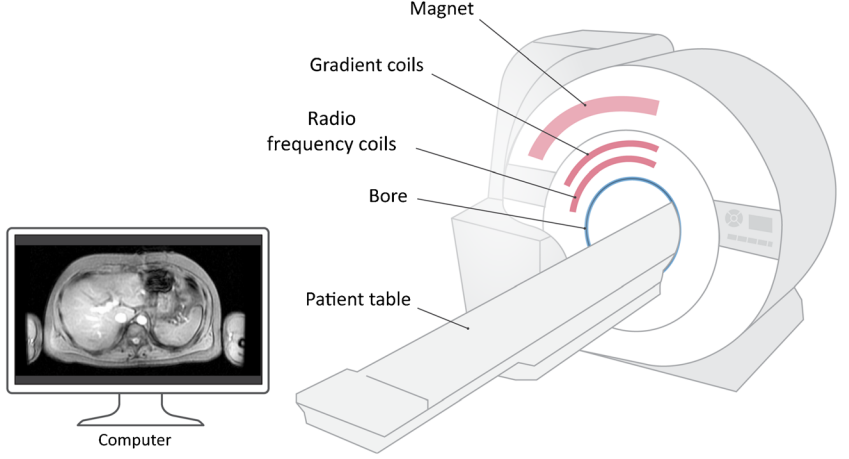
\includegraphics[width=\linewidth]{./Images/MRI-Schematic.png} 
 	\caption{Schematic of an MRI scanner taken from~\cite{Serai2021}.}
 	\label{fig:MRISchematic}
 \end{figure} 

\subsection{Magnetic Excitation and Relaxation} \label{SubSec:MagneticExcitationAndRelaxation}
%In the following section, the basic principles underlying MR imaging are presented. These include the relation between RF excitation and relaxation.
The base principles behind MR imaging are RF excitation and relaxation. Through these, the raw k-space data is measured which enable the reconstruction to an image. Terminology such as $T_1$ and $T_2$ relaxation times are introduced and explained. These are the basis for the pulse sequence discussed in section~\ref{SubSec:ImageAcquisitionAndK-Space}.

\subsubsection{Radio Frequency Excitation}
Individual nuclei precess around the field $B_0$ at a
resonance frequency known as the Larmor frequency $\omega_0$ of the net magnetization vector, which generally occurs in the RF range of the electromagnetic spectrum and is related to the external magnetic field as:
\begin{equation} \label{eq:LarmorFrequency}
	\omega_0 = \gamma \cdot B_0,
\end{equation}
with $\gamma$ being the gyromagnetic ratio, which is a fixed value depending on the nuclei~\cite{SamplingStrategies}. When nuclei are placed in the presence of a strong static magnetic field such as $B_0$ the nuclei split into two energy states, either aligned parallel to the magnetic field $B_0$ (called a spin-up state) or aligned anti-parallel to $B_0$ (called a spin-down state). The spin-up state has a slightly lower energy level as compared to the spin-down state and is therefore preferred. This slight difference in the spin states ($0.001\%$) results in an overall net magnetization $M$ aligned in the same direction as $B_0$. \\
To create an MR signal, the spins are excited out of their resting equilibrium, i.e. tipping $M$ away from $B_0$. To detect the signal from the hydrogen nuclei in the tissues an additional external field $B_1$ is introduced at the resonant Larmor frequency $\omega_0$ that can affect magnetization vector, causing it to rotate into a plane orthogonal to its original orientation. The rotated vector continues to precess around the $B_0$. The precession of the magnetization vector in the transverse plane can be detected by an RF coil tuned to the resonant frequency $\omega_0$. RF coils can be operated in a receive-only mode, in which case the inherent body coil is used as a transmitter; or the RF coils can be both transmit and receive. The purpose of the RF transmit coil is to create a time-varying $B_1$ field at right angles to $B_0$ that could be linearly or circularly polarized. The closer the receiving coil is to the source of the MR signal, the better the signal-to-noise ratio (SNR). Receiver coils generally comprise arrays of smaller individual coils or elements; however, each individual coil element has a limited depth penetration. \\
Multiple arrays of coils, termed phased-array coils, can be used together to achieve a higher coverage. The multiple coils are electronically decoupled from one another so that they do not appear as just a single large coil. The images from individual coils are independently reconstructed and then grouped together to create the final image. An RF pulse of amplitude $B_1$, called excitation pulse, is applied for a certain time duration to tip the magnetization at an angle away from the $B_0$ field. The precessing transverse magnetization induces a voltage in the receiver RF coil; this induced voltage is known as the free induction decay. After the pulse, the magnetization returns to thermal equilibrium by processes known as MR relaxation. To fully encode the spatial information within the field of view (FOV), pulse sequences must be iterated numerous times. The time between successive iterations of a pulse sequence is known as the repetition time (TR). The time between the application of the initial RF pulse and the middle of the detected echo is known as the echo time (TE). Due to this the overall time to acquire an MR image is quite long~\cite{Serai2021}.\\

\subsubsection{Magnetic Relaxation}
Once the RF pulse is turned off, $M$ continues to precess as it returns to its thermal equilibrium state. During this time, two types of relaxation occur: $\text{T}_1$ (longitudinal or spin lattice) and $\text{T}_2$ (transverse or spin/spin). One attribute that makes $\text{T}_1$ and $\text{T}_2$ so valuable for determining the signal in MRI is their sensitivity to the presence and type of tissue. It is this tissue dependence property that gives MR its excellent soft-tissue contrast. $\text{T}_1$ relaxation describes the recovery of the longitudinal magnetization back to thermal equilibrium following a perturbation by an RF pulse. The longitudinal component regrows along the Z direction with a time constant $\text{T}_1$. In other words, after the RF pulse is turned off, the protons that were disturbed give their energy to the surrounding environment and return back to their original equilibrium state, realigning with $B_0$. Hence, $\text{T}_1$ relaxation is also called longitudinal relaxation. Furthermore, because $\text{T}_1$ relaxation involves the loss of energy that was put into the spin system by the RF pulse, it is also referred to as spin-lattice relaxation, the lattice consisting of surrounding macromolecules. This loss of energy is stimulated by the fluctuating magnetic fields associated with the dipole–dipole interactions of neighboring magnetic moments. $\text{T}_1$ relaxation can only occur when these magnetic field fluctuations occur at the resonant frequency $\omega_0$. The rate at which the spin magnetization $M_z$ recovers to $M_0$ at time $t$ is called $\text{T}_1$ relaxation time. It can be expressed as follows:
\begin{equation}
	M_z = M_0 \cdot \bigg(1 - e^{-\frac{t}{\text{T}_1}} \bigg).
\end{equation}
A preferred method of measuring $\text{T}_1$ relaxation is the Look-Locker method, which is based on the principle that one does not need to wait for the net magnetization vector to equilibrate in order to measure $\text{T}_1$. Instead, an RF pulse is used with a small flip, which can be repeatedly applied. The acquisition pulse sequence is designed to generate a train of signals that gradually approaches a steady-state recovery. The recovery curve measured by this technique can be fitted to an exponential curve to provide an effective $\text{T}_1$ measurement. This has become one of the most popular $\text{T}_1$-mapping method for abdomen and cardiac imaging. The general principle of $\text{T}_1$ mapping is to acquire multiple images with different $\text{T}_1$ weightings and to fit the signal intensities of the images to the equation of $\text{T}_1$ relaxation. $\text{T}_1$ relaxation values for tissues can be estimated by fitting the data to the following equation:
\begin{equation}
	S = S_0 \cdot \bigg(1 - A \cdot e^{\frac{\text{TI}}{\text{T}_1}} \bigg),
\end{equation}
where $S$ is the signal intensity measured at each inversion time value $\text{TI}$, $S_0$ is the initial signal intensity at time $t=0$ and $A$ is
a constant.\\
$\text{T}_2$ relaxation results in the loss of transverse magnetization caused by interactions between the magnetic fields of neighboring hydrogen nuclei. It is not an energy loss process like $\text{T}_1$ but is a loss of phase coherence within the spin system. This process, also known as spin-spin relaxation, leads to the destruction of transverse magnetization and causes the magnetic moments of the tissue to dephase. $\text{T}_2$ mapping is a method of measuring the $\text{T}_2$ value of the tissue. $\text{T}_2$ relaxation time can be calculated using a $\text{T}_2$ sequence with different echo times (TEs). The most fundamental sequence for $\text{T}_2$ mapping is signal measured with spin echo techniques (multiple sequences with different TE values). Other 2-D sequences have been used, such as multi-echo spin echo (MSME) and fast spin echo (FSE). Synthetic MRI is another quantitative method in which a single saturation recovery turbo spin-echo sequence is used to estimate $\text{T}_2$ transverse relaxation. $\text{T}_2$ relaxation values for tissues can be estimated by fitting the data to the following equation using a mono-exponential decay curve:
\begin{equation}
	S(\text{TE}) = S_0 \cdot e^{\frac{\text{TI}}{\text{T}_2}},
\end{equation}
where $S(\text{TE})$ is the signal intensity measured at each $TE$ and
$S_0$ is the initial signal intensity at time $t=0$.

\subsection{Image Acquisition and the Concept of K-Space} \label{SubSec:ImageAcquisitionAndK-Space}
After discussing the physical mechanisms behind MRI, it is time to look at the actual process of acquiring the image as well as the concept of the k-space. 
%\subsection{Image Acquisition and Pulse Sequences}
The image contrast in MR imaging arises from tissues generating MR signals with different intensities due to their physical properties. Contrast weighting of the MR signal is obtained by the design of pulse sequences, which consist of repetitive trains of RF pulses. Two of the most common pulse sequences are gradient echo 
%(GE) 
and spin echo 
%(SE) 
sequences. %\\

\subsubsection{Gradient Echo Sequence}
In a gradient echo (GE) sequence, the free induction decay (FID) signal is manipulated by a bi-polar gradient. The excitation pulse tilts the magnetization by $\alpha$ degrees. For $\alpha = 90°$ the longitudinal magnetization is rotated in the transverse plane. The data is sampled during a gradient echo at time TE after the excitation pulse. This gradient echo is achieved by dephasing the spins with a negative gradient before they are rephased by an opposite gradient with opposite polarity to generate an echo. A schematic overview of the process can be seen in Figure~\ref{fig:GradientEcho}. \\
The pulse sequence is repeated a number of times to acquire the entire image. 
%The time between two excitation pulses is called the repetition time. 
Changing the TR, TE, and flip angles of a GE sequence influences the contrast weighting. $\text{T}^*_2$-weighted contrast can be achieved by using small flip angles and a long TE and moderate TR. By using large flip angles, a short TR and a short TE, a $\text{T}_1$-weighted signal can be acquired. Using small flip angles in combination with a long TR and a short TE generates proton density contrast~\cite{PulseSequences}.%\\

\begin{figure}[htpb]
	\centering
	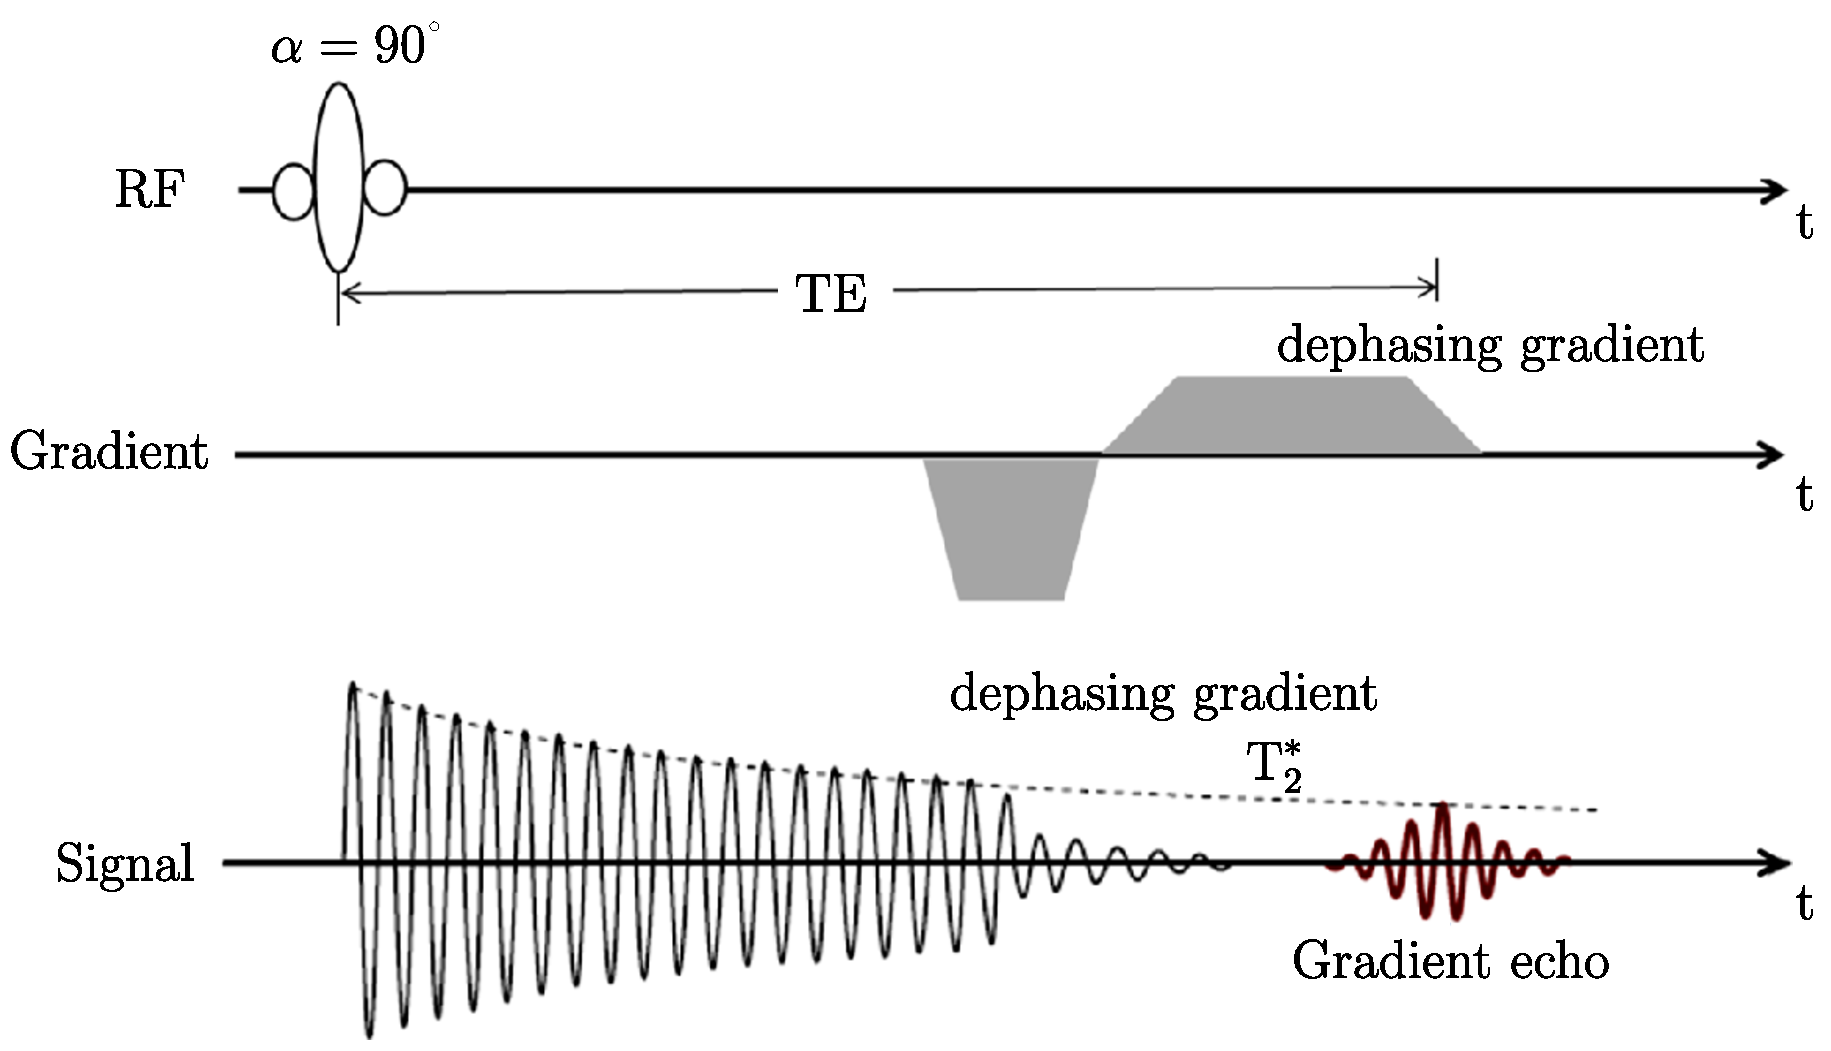
\includegraphics[width=\linewidth]{./Images/GradientEcho.pdf} 
	\caption{Schematic of an gradient echo sequence taken from~\cite{PulseSequences}.}
	\label{fig:GradientEcho}
\end{figure}

\subsubsection{Spin Echo Sequence}
With a spin echo (SE) sequence, pure $\text{T}_2$-weighted contrast can be generated. When a $90°$ pulse rotates the magnetization into the transverse plane, the resulting FID signal quickly decays due to the strong $\text{T}^*_2$ dephasing. If after a time $\frac{\text{TE}}{2}$ a $180°$ pulse is applied, the spins will be flipped and start to rephase. After another time, $\frac{\text{TE}}{2}$, a measurable echo signal is created. The spin dephasing due to static magnetic field inhomogeneities is compensated by inverting the spins with the $180°$ refocusing pulse. This process is visualized in Figure~\ref{fig:SpinEcho}.\\
Consequently, the decay of the signal at time TE will solely originate from the $\text{T}_2$ relaxation. A SE sequence can also be used to generate proton density or $\text{T}_1$-weighted signals by using a short TE and a long or short TR, respectively~\cite{PulseSequences}.

\begin{figure}[htpb]
	\centering
	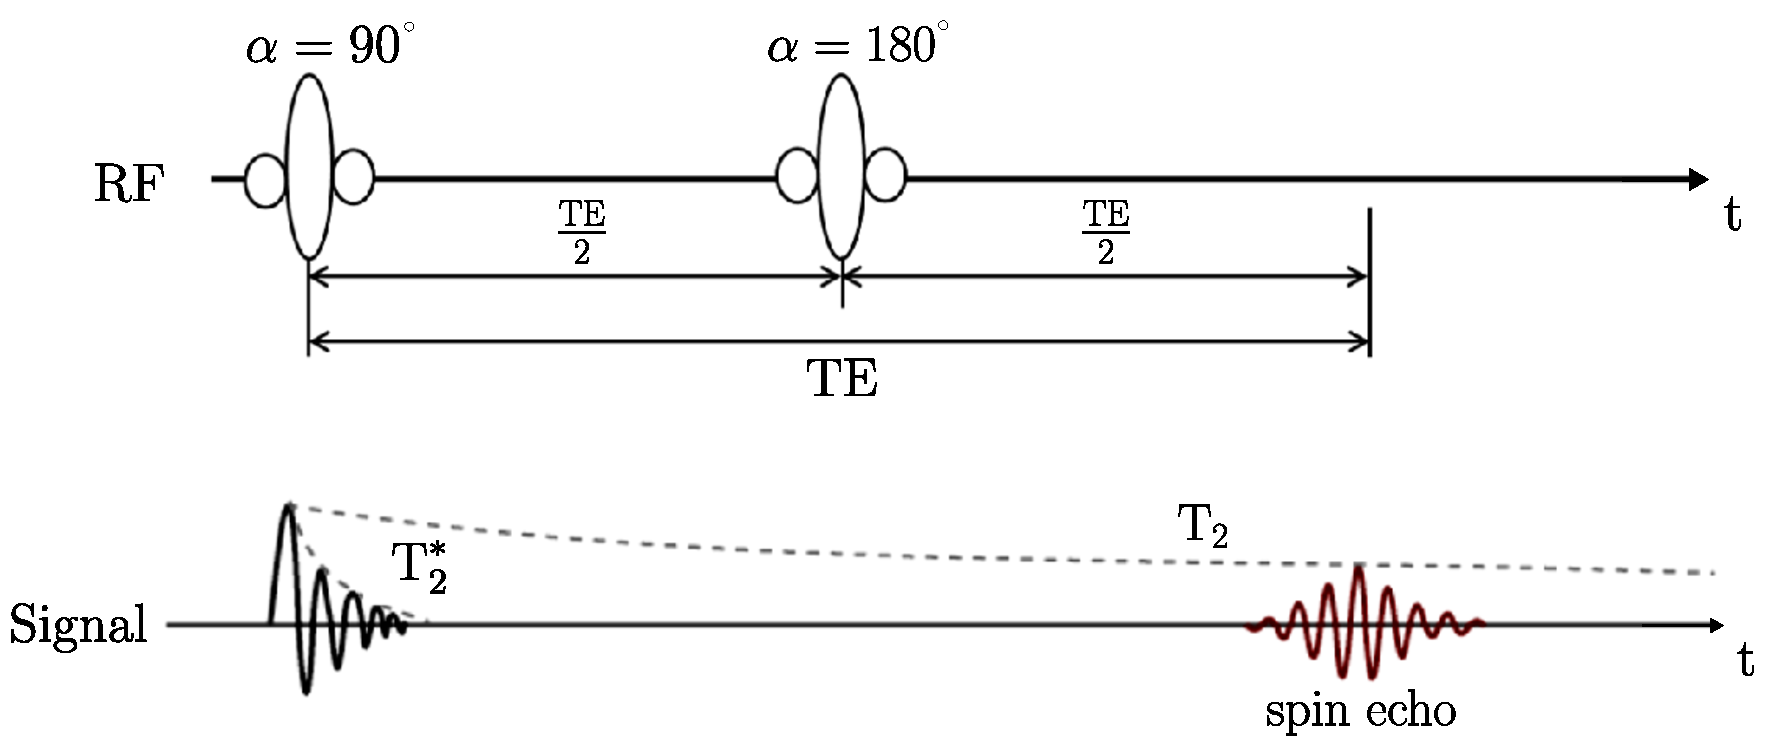
\includegraphics[width=\linewidth]{./Images/SpinEcho.pdf} 
	\caption{Schematic of an spin echo sequence taken from~\cite{PulseSequences}.}
	\label{fig:SpinEcho}
\end{figure}


\subsubsection{Introduction to K-Space}
The concept of the k-space is a generalization of the simple relation of a time-variant signal to a spectrum of two or more dimensions. An 2D image is related to a 2D k-space data set by a 2D FT, as seen in Figure~\ref{fig:2D_MRI_Measurement}
%, same as a 1D spectrum is related to the 1D signal by a normal (1D) FT. A 2D FT can be achieved by applying the (1D) FT successively row-by-row and column-by-column. 
As the FT is an information-preserving operation, the k-space data contains exactly the same information as the image data. Thus, in order to get the full image information, the full k-space data needs to be measured. The task of forming an image by this approach is then converted to the task of finding a way to measure the necessary corresponding k-space data. 
%An understanding of the physical meaning of the k-space domain can be derived from Figure~\ref{fig:1D_MRI_Measurement}. The time-domain signal defines the 1D k-space. Its coordinates are defined by the area under the gradient which the spins have experienced prior to the collection of each k-space data-point. 
Using the Larmor frequency again from Equation~\ref{eq:LarmorFrequency} the coordinates in 2D k-space will thus be given as $k_x = \gamma \cdot G_x \cdot t$ and $k_y = \gamma \cdot G_y \cdot t$. \\
In order to acquire an MR image, methods need to be developed 
%in order to get from one k-space point to the next. 
to traverse the k-space.
There are only two possibilities as seen in Figure~\ref{fig:kSpaceTrajectories}. The first one is to apply a gradient, in which case the k-space trajectory will be a line defined by the orientation of the gradient (see Figure~\ref{fig:constant_k-space_gradient}). As long as the gradient is kept constant, the k-space trajectory will be a straight line. 
%This way it is easy to see why simple superposition of two gradients will not produce an image. The resulting k-space trajectory will merely represent a straight line traversing k-space at some skewed angle. \\
The second method for traversing the k-space is the application of a refocusing pulse, which will lead to a jump of the k-space trajectory around the origin (see Figure~\ref{fig:refocusing_k-sapce_pulse}). It is clear that a spin-echo formation alone will not allow coverage of all of the k-space, since the trajectory would only jump between the two mirror symmetric points. A combination of spin echoes and gradients can, however, produce very efficient k-space trajectories. All of the existing k-space-based imaging techniques are based on some combination of these two basic means of traversing the k-space. \\
Is should be noted that the signals are measured 
%not continuously, but 
at discrete time intervals called the dwell-time of data acquisition. This discrete sampling leads to an ambiguous assignment of frequencies above a given threshold which is called the Nyquist frequency. The Nyquist frequency therefore determines the acquisition bandwidth inside which the signal should occur. The definition of the k-space coordinates implies that these are invariant with respect to the actual strength of the gradient used, as long as $G$ and $t$ are constant. Mathematically, data acquisition under a strong gradient and in a shorter acquisition time will yield the same k-space data and thus the same image as acquisition under a weaker gradient and a longer acquisition time. A shorter acquisition time and a closer spacing of sampling points are equivalent to a higher-acquisition bandwidth. Since the received noise grows with the square root of the bandwidth, a faster imaging technique will therefore by principle always carry the penalty of a lower signal-to-noise ratio (SNR)
%, even if all other factors influencing high-speed imaging are neglected. \\
For a conventional spin-echo imaging sequence
%, which is still widely used, 
a typical acquisition time of 5 to 10~ms for each phase-encoding step is used. Acquisition of 
%typically 
192 to 256 phase-encoding steps therefore requires a total net acquisition time of 1 to 2~s. However, this is much shorter than the 
%total 
actual
acquisition time of such a sequence, which is determined by the repetition time defined by the $\text{T}_1$-contrast. 
%From the aforementioned general considerations 
It 
%immediately 
follows that the SNR of a fast imaging sequence leading to acquisition times of approximately 50~ms, will be lowered by at least a factor of 5 to 10, regardless of the actual sequence used. 
%Fast imaging therefore requires improved SNR provided by radio-frequency coil designs. The improvement in SNR driven by the need for fast imaging will also benefit slower techniques, providing images with better spatial resolution and/or higher SNR. 
Fast imaging thus relies on radio-frequency coil designs improving the SNR.\\
The discrete data sampling has some additional consequences regarding the sampling density and coverage of data in k-space. Different parts of the k-space encode different features of the image: The center of the k-space hold the lower frequencies which represent the image contrast, whereas the outer parts encode the higher frequencies for sharp structures. Due to the symmetry of the 2D FT, this statement can also be reversed: The image center will be encoded by low-resolution k-space data. Therefore, sampling of sparsely distributed k-space data will reduce the effective field of view of the final image. \\
Mathematically, the final image will look exactly the same, irrespective of the way the data is sampled in the k-space. In practice, however, different approaches 
%to sampling 
can have a major impact on image quality
%. This is due to the fact that sampling 
as the data has to 
%proceed 
sampled
sequentially. The observed spins evolve not only as a function of the gradients defining the intended k-space trajectory, but are also influenced by other mechanisms unrelated to image encoding. It is noteworthy that the coordinates in k-space are expressed in units of a phase angle across space. Any mechanism affecting the phase of the signal along this trajectory will therefore alter the k-space trajectory. Some such commonly occurring mechanisms are flow and motion effects, magnetic field inhomogeneities, as well as susceptibility and chemical shift effects. The consequence of such phase effects in terms of imaging properties is dependent on the particular sequence and data sampling speed. In addition to phase effects, the signal decay with $\text{T}_2$ needs to be taken into account also, especially if the data acquisition time is similar or even longer than the $\text{T}_2$ of the observed tissues under construction~\cite{SamplingStrategies}.

\begin{figure}[h] %tpb
	\centering
	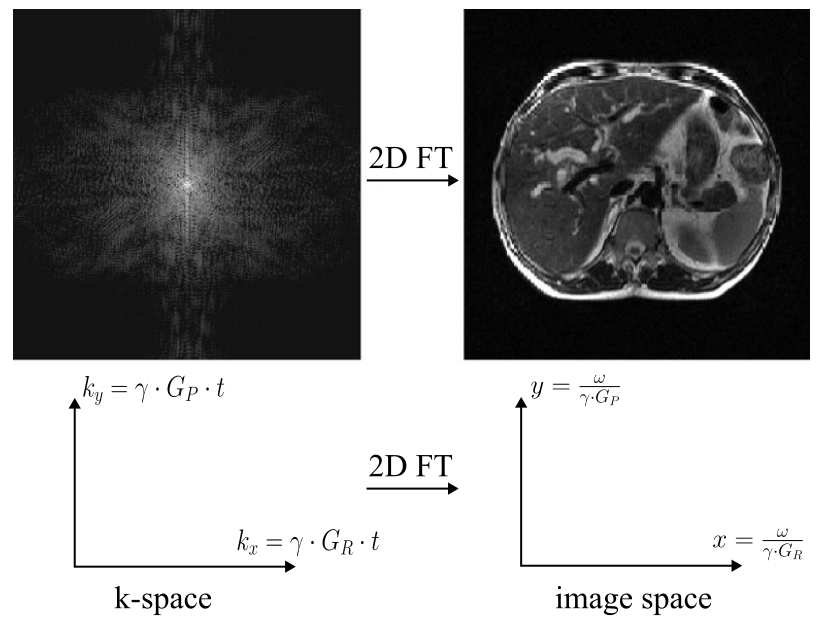
\includegraphics[width=\linewidth]{./Images/2D_MRI_Measurement.png} 
	\caption{Correspondence of the image domain and the k-space via a 2D FT, adapted from~\cite{SamplingStrategies}. The coordinates of each domain are defined by the Larmor frequency according to Equation~\ref{eq:LarmorFrequency}.}
	\label{fig:2D_MRI_Measurement}
\end{figure}

\begin{figure}[h] %tpb
	\centering
	\begin{subfigure}{0.445\textwidth}
    		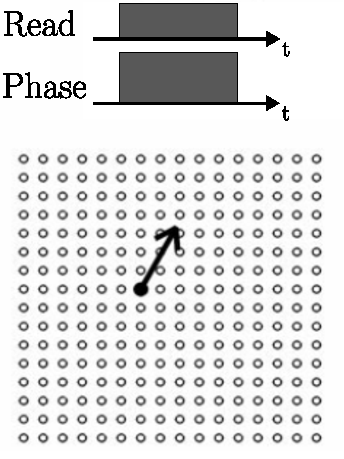
\includegraphics[width=\textwidth]{./Images/ConstantGradient.pdf}
    		\caption{Schematic of a constant gradient creating a straight k-space trajectory.}
    		\label{fig:constant_k-space_gradient}
	\end{subfigure}
	\hfill
	\begin{subfigure}{0.445\textwidth}
    		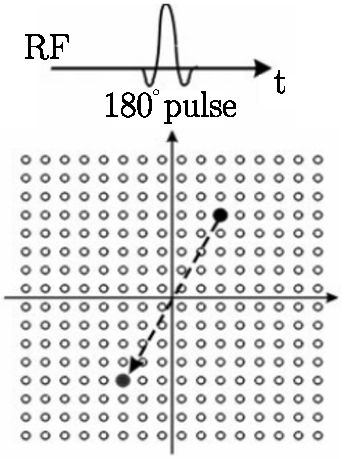
\includegraphics[width=\textwidth]{./Images/RefocusingPulse.pdf}
    		\caption{Schematic of an refocusing pulse inverting the phase of the k-space.}
    		\label{fig:refocusing_k-sapce_pulse}
	\end{subfigure}
	\caption{Methods of moving in the k-space using a) constant gradients to move along straight lines or b) mirror the k-space at the origin using a refocusing pulse. Adapted from~\cite{SamplingStrategies}.}
	\label{fig:kSpaceTrajectories}
\end{figure}

\subsubsection{Rectilinear K-Space Sampling}
Almost all MR imaging sequences 
%used in clinical routine presently 
are based on rectilinear k-space sampling, i. e., the sampling points 
%in k-space 
are placed on a rectangular grid. This 
ia also referred to as Cartesian sampling and 
%reflects the ability to use a 
allows the usage of the fast Fourier transform (FFT) 
%for such a sampling strategy. It allows 
which enables 
image reconstruction in 
%considerably under 1~s
a very short time (under 1~s). 
%With special reconstruction processors, the reconstruction speed can be as high as 10 to 25 images per second. 
For comparison, using
the 
%general 
2D FT 
to transform a non-rectilinear grid can take about
%for transformation of a comparable number of non-rectilinear grid points in comparison requires
5 to 50~min per image~\cite{SamplingStrategies}.
%, using identical computer hardware. \\
In a Cartesian acquisition, one or more lines of k-space parallel to a Cartesian axis are collected following application of an RF pulse and generation of an RF echo. Adjacent points in a single line are collected in rapid succession in a single echo. The time between echoes and adjacent lines is much slower. The direction of fast acquisition is known as the frequency direction and the other one or two directions are known as the phase-encode direction or directions. Following line-by-line filling of k-space in a Cartesian sequence, each layer of a filled grid is subsequently used to reconstruct a single image slice~\cite{Bardo2021}.

%%% Old from Henning (to detailed....)
%Utilizing the two means of traversing the k-space, 
%%the basic techniques for 
%rectilinear sampling can be divided into spin-echo-based techniques and gradient-echo-based techniques. In all rectilinear sampling techniques, the gradient which is used during signal acquisition is commonly called the readout gradient, whereas gradients used to bring the k-space trajectory to a certain starting point before data acquisition are called phase-encoding gradients. \\
%A gradient echo is formed using a reversal of the readout gradient. In conventional gradient-echo imaging, only the refocusing part of the k-space trajectory is measured, whereas the signal dephasing as well as phase encoding is performed prior to data acquisition (Fig. 8). The experiment is repeated after the recovery time TR, using different offsets of the phase-encoding gradient prior to each acquisition step. Using the k-space, it can be easily seen how gradient-echo imaging can be generalized to a faster technique, using less excitation periods by sampling more than one k-space line after each excitation. Repeating gradient reversal and the application of a phase-encoding gradient can be used to read out several k-lines per acquisition with a concordant reduction in total imaging time. In the extreme case, all k-space data can be read out following a single excitation. This is called the single-shot, echo-planar imaging (EPI) sequence~\cite{EPI}. \\
%%Historically, the development took place the other way round: EPI was first invented by P. Mansfield, and gradient echoes followed several years later. The concept of the k-space was not widely known at that time, therefore, the intrinsic relationship between the two techniques has only been acknowledged gradually. 
%Despite the close conceptional similarity between EPI and gradient echo techniques
%%with respect to their k-space trajectories
%, both types of sequences have vastly different imaging and hardware implications. This difference is caused by the sequential sampling of k-space points and the resulting influences on the signal of the mechanisms mentioned previously. As the signal decays with $\text{T}_2$ the signal amplitude is reduced during data acquisition. For conventional gradient-echo imaging, even with moderate gradient strength (and thus longer acquisition times), this effect is inconsequential since the typical acquisition times of 5 to 10~ms are considerably shorter than the typical $\text{T}_2$ of tissues. For EPI, however, the total acquisition time for n k-space lines is n times longer, even if the time necessary for gradient reversal and phase encoding is neglected. For the moderate acquisition times noted previously, this will lead to total acquisition times of 1~s or more, which exceeds most $\text{T}_2$ values observed in human tissues. 
%%Dephasing of spins across the selected slice will lead to $\text{T}_2$ of the order of 100~ms at most. 
%For identical acquisition times, as in our gradient-echo example, the signal will have vanished long before the end of data acquisition leading to information loss. 
%%Depending on whether data acquisition has commenced at the center or in the outskirts of k-space, the resulting image will either be severely blurred or reveal merely contours without contrast. This illustrates that 
%Thus EPI 
%%absolutely 
%requires very fast data acquisition in order to 
%%acquire 
%scan all of the k-space data within 
%%not much more than 100~ms at most; otherwise, 
%100~ms or else image quality will deteriorate significantly. In the given time range, state-of-the-art scanners can acquire 64 to 128 phase-encoding steps. Longer acquisition times allowing for higher 
%%nominal 
%resolution are of course technically feasible, but the $\text{T}_2$-decay 
%%of the signal will 
%prohibits the realization of this 
%%nominal 
%resolution. 
%%Since cerebral spinal fluid (CSF) has a long $\text{T}_2$, EPI images of the head with long acquisition times can look deceptively sharp. It must be noted, however, that the perceived sharpness applies only to CSF-filled structures, whereas the true resolution of parenchyma with a $\text{T}_2$ of approximately 60~ms is considerably worse. 
%With even stronger and faster gradients it is 
%%of course feasible 
%possible to acquire true high-resolution images with short acquisition times, but the penalty in SNR for such applications is too severe and has prohibited its use for most forms of morphological imaging. The EPI technique has emerged, however, as an ideal vehicle for functional imaging either in BOLD-based fMRI, in first-pass perfusion measurements or in diffusion imaging, but it is not a viable technique for high-resolution morphological imaging~\cite{SamplingStrategies}.\\
%Even for short acquisition times, EPI suffers from severe problems regarding its imaging properties, which are caused by the phase-altering mechanisms mentioned previously. Chemical shift effects and susceptibility both lead to signal phase shifts which increase linearly with time. Since data acquisition along the readout gradient is fast, there is little effect in the readout direction. In the phase-encoding direction, however, the dwell time amounts to the acquisition time of one k-space line. 
%%For the acquisition of 64 k-space lines in 64~ms, the field of view in frequency units will be 1000~Hz. For a frequency shift of fat vs water of approximately 200~Hz at 1.5~T, this will mean that the signal of fatty tissue will be shifted by 20$\%$ of the image width. The resulting misregistration artifact necessitates the use of fat suppression for practically all EPI applications. 
%Field inhomogeneity and susceptibility will lead to a similar shift. Since the resulting frequency shifts are not as discrete as chemical shift effects, the misregistration will vary continuously leading to highly non-linear image deformations. An additional problem in EPI relates to the fact that the k-space trajectory runs in opposite directions in every other k-space line due to the alternating polarity of the readout gradient. Any asymmetry in the acquired data will therefore lead to some slight perturbation in any other line known as the $180°$ artifact.  
%%The final image will therefore be a superposition of the true image with an image representing the perturbation in every other k-space line. From this discussion of the k-space trajectory, it is easy to see that this perturbation will generate an image which is displaced by half the field of view in the phase-encoding direction. This is the so-called $180°$ artifact.
%\\All the confounding factors discussed will produce such artifact. With appropriate post-processing routines based on reference signals, some of the sources of artifacts can be corrected for. In general, the $180°$ ghost will become stronger whenever any of the mechanisms mentioned previously become significant and will therefore deteriorate the image quality further. Motion can also cause phase-effects on the signal. With an alternating readout gradient, motion along this direction will be refocused in every even refocusing period. Consequently, a flow-dependent $180°$ ghost will occur. Motion along the phase-encoding direction will lead to a velocity-dependent increase in the signal phase and consequently to a velocity-dependent signal displacement. 
%%Signal from a round vessel with laminar flow will therefore appear as a boomerang-shaped artifact displaced from the vessel wall. Any vascular diagnosis based on EPI images therefore has to be made with the utmost care. The inherent artifact behavior limits the practical use of EPI to examinations of the head. Abdominal or thoracic EPI and even cardiac EPI have not been developed beyond a feasibility state. They require considerable efforts in region-selective shimming and even post-processing, using actual field maps of the patient such that the time advantage of EPI is lost. 
%Thus, for the time being, EPI 
%%therefore has to be
%is regarded as a brain-only technique 
%%where it serves as a vehicle for the 
%for fMRI applications, including diffusion and perfusion imaging~\cite{SamplingStrategies}.\\
%Conventional gradient-echo imaging suffers from no such effects and can therefore be applied all over the body with no or only mild susceptibility misregistration. Chemical shift effects will, however, influence the contrast of gradient-echo images by the chemical-shift-dependent dephasing of fat and water signals. Signals from fat and water protons located at the same position will periodically be in- and out of phase with each other in a time interval determined by their difference in Larmor frequencies. 
%%For 1.5~T the time difference between the two extreme conditions will be approximately 2.5~ms. Images acquired with TEs differing by 2.5~ms will look dramatically different due to this effect, although $\text{T}_2$-dependent effects for such small TE differences will be negligible. 
%As shown in Fig. 11, the out-of phase image will show a considerable reduction in signal amplitude in tissues containing both fat and water protons such as bone marrow. In addition, an artificial black line will appear at the interface between fatty and water tissues due to the zero crossing of the signal between these antiphasic images. When (im)properly used, this artifact can be used to beautify images, giving them a crisp and well-defined appearance. Care must be taken, however, not to mis-read this artifact as an anatomical structure. With respect to the total acquisition time, gradient-echo imaging is somewhat slower than EPI due to the necessity of repetitive application of excitation pulses. Gradient-echo sequences, which are optimized for speed, typically achieve imaging times of 200 to 400~ms, using gradient systems comparable to those of EPI. Due to the strong signal saturation caused by the very short repetition times, the intrinsic SNR is comparably low. \\
%%(but for many applications still satisfactory). 
%%The SNR can be optimized by using low-excitation flip angles and/or total signal refocusing (true FISP). In combination with bolus application of contrast agent, gradient-echo sequences allow the acquisition of MR angiograms especially of the thorax, abdomen, and the extremities with unprecedented image quality. This  relatively new application has led to whole new field of applications for gradient-echo imaging. \\
%In order to reach a compromise between the more efficient sampling of EPI and the much more benign artifact behavior of gradient echoes, 
%%segmented 
%mixed approaches have been developed. In these approaches, more than one excitation is used and several k-lines are sampled per excitation. 
%%Depending more on the perspective of their creators than on anything else, such approaches are called multi-echo gradient echo, multi-shot EPI, or segmented EPI. 
%The optimum number of k-lines per excitation is strongly dependent on the particular application
%%; it 
%and can range from 3 for MR angiography and cardiac imaging to 64 or more for high-resolution head imaging.

%\subsection{Spin-Echo Techniques}
%In spin-echo techniques, refocusing pulses are used in the construction of the k-space trajectory. Conventional spin-echo techniques acquiring one k-line per excitation are identical to gradient-echo techniques with respect to the k-space sampling strategy used. In rapid acquisition relation enhanced imaging (RARE, e. g., turbo spin echo and fast spin echo), multiple refocusing pulses are employed in order to sample more than one and, in the extreme case, all k-lines per excitation [15]. In order to suppress unwanted coherences, the k-space trajectory in RARE has to be brought to the identical position at the time of application of each refocusing pulse. This is achieved by using a phase-encoding rewinder after reading out each k-line (Fig. 12). Conceptionally, RARE is very similar to EPI, however,
%%and the possibility to build a spin-echo-based technique has already been mentioned in the original paper by Mansfield. 
%The spin-echo refocusing makes a huge difference with respect to the artifact behavior. For once it should be noted that the direction of data sampling is identical for all k-lines. Therefore, no $180°$ ghosts will occur. In addition, all phase changes caused by chemical shift, susceptibility, etc., are refocused. The phase effects therefore do not accumulate but re-start in each k-line just like in conventional spin-echo sequences. Motion effects are in principle similar to the ones discussed for EPI with a refocusing of flow in every even echo. Since for low flow the resulting $180°$ effect will be weak, and for high-flow velocity the signal will vanish from the image due to outflow during the echo train, the resulting flow artifact behavior of RARE is very benign. 
%%Slow-flow vessels (e. g. liver veins), which are black on conventional spin-echo imaging, appear very bright on $\text{T}_2$-weighted RARE imaging due to this even echo refocusing effect.
%The insensitivity to other mechanisms leads to $\text{T}_1$ and $\text{T}_2$ as the basic contrast mechanism for RARE. From the discussion of the properties of k-space it follows that the $\text{T}_2$-contrast is determined by the echo times of the acquisition of the k-lines with low phase encoding. The $\text{T}_2$-contrast of a given implementation can thus be varied widely by changing the order of the phase-encoding gradient. By similar consideration, $\text{T}_2$-relaxation along the echo train leads to a loss of resolution when the k-lines carrying the edge information are acquired at long echo times. For most diagnostic applications in high-resolution imaging, a segmented acquisition is therefore preferred with echo train lengths ranging between 8 and 35 for $\text{T}_2$-weighted scans and 3 to 5 for $\text{T}_1$-weighted scans. Nevertheless, single-shot variants are also being used~\cite{SamplingStrategies}. 
%%Especially single-shot RARE (or single-shot FSE) with very strong $\text{T}_2$-contrast has been shown to be extremely useful for imaging of liquid-filled structures like in MR myelography [16], MR urography [17], or MR cholangio-pancreatography (MRCP) [18]. 
%Using half-Fourier phase encoding in half-Fourier acquired single-shot turbo spin echo (HASTE) [19], single-shot implementations with less $\text{T}_2$-contrast are also feasible. It has been noted that signal from fat is significantly brighter in RARE compared with conventional spin-echo imaging at equal echo times [20]. This is due to so-called J coupling of protons in lipids, which leads to a periodic modulation of their resonances just like the modulations caused by two elastically coupled pendulums [21]. This modulation will not be refocused but continue despite the reversal of the phase by the 180 pulse (Fig. 13). At a time interval equal to 1/(2 J), the signals from such coupled spins will be opposed and therefore canceled. For typical coupling constants, this condition is reached at echo times of 80 to 140 ms typically used for $\text{T}_2$-weighted imaging. The multiple refocusing in an echo train ensures that the phase of the signals from coupled spins stay together along the echo train; thereby, signal suppression is avoided and fat will appear bright. A similar cause is implied for a relative reduction in susceptibility contrast on RARE images (Fig. 14). Static susceptibility effect will be refocused on both spin-echo sequences. If spins move along strong local gradients as caused by hemorrhage, for example, the motion-dependent variation of their Larmor frequency cannot be refocused due to the random nature of the motion. Multiple refocusing pulses, however, will ensure that the spin phases stay together. Some such diffusion-dependent dynamic susceptibility effect is observed in most organs (nuclei in the brain and basal ganglia, liver, lung, etc.). Therefore, RARE images can look very different from conventional spin-echo images at identical echo times. Due to the repetitive use of refocusing pulses and the necessity for rewinding the phase-encoding gradient, RARE is inherently slower than EPI. The gradient performance of current scanners allows refocusing intervals as short as 4 ms or less. The high radio-frequency power inherent to a long train of $180°$ pulses limits, however, the range of applications for such fast echo trains. Even though this problem can be ameliorated by the use of lower refocusing flip angles, EPI with typical readout times of 1 ms or less will remain faster. The big advantage of spin-echo techniques remains, however, their lack of distorting artifacts which makes spin-echo techniques applicable all over the body. Even high-quality cardiac images with HASTE have been demonstrated as well as perfusion and ventilation imaging of the lung [22].

\subsubsection{Non-Rectilinear K-Space Sampling}
A common problem of rectilinear sampling techniques is the very heterogeneous nature of the k-space trajectories used: Data are acquired along straight k-space lines under a constant gradient. Going around the corner of the trajectory requires very fast switching for a brief period. 
This 
%The combination of both modes of operation 
is very demanding on the gradient power amplifiers, which have to be able to alternate between the two modes. A more common load on the gradients is offered by the use of curved k-space trajectories. Especially spiral trajectories~\cite{SpiralMRI, SpiralMRI2} have won considerable interest due to their very efficient use of the gradient system. 
%For a given gradient system it is also possible to calculate the trajectory achieved by running the gradient system always under full load. In terms of the gradient performance, spirals therefore are considerably more efficient than rectilinear k-space trajectories. 
A practical problem relates to image reconstruction which requires algorithms not (yet) commonly available and which can take several seconds per image on a typical scanner~\cite{SamplingStrategies}. 
%In order to make use of the very fast FFT algorithm, the typical approach to reconstruction of data sets acquired with spiral (or other non-rectilinear) trajectories is to first interpolate the data onto a rectilinear grid and then to use FFT for the reconstruction itself. With further developments of spirals, it is expected that reconstruction algorithms will become widely available. 
The ultimate success of spiral imaging will then be determined by its inherent imaging properties, which are significantly different from rectilinear scans. Constant off-resonance effects, such as chemical shift, field inhomogeneity, and susceptibility, will not lead to a displacement in the phase-encoding direction, but to blurring of the corresponding structures~\cite{SamplingStrategies}.
%Firstly, it should be noted that spirals do not have a preferred orientation like the readout- and phase-encoding direction in rectilinear scans. Constant off-resonance effects, such as chemical shift, field inhomogeneity, and susceptibility, will therefore not lead to a displacement in the phase-encoding direction. It will instead lead to blurring of the corresponding structures~\cite{SamplingStrategies}. 
%In some respects this can be regarded as an advantage since the severe distortions of EPI images are avoided. On the other hand, some mild distortion in EPI images can be tolerable for most applications, whereas blurring artifacts are not. \\
%These artifacts can be avoided if the off-resonance frequency is known. The data can then be corrected and a sharp image will be produced. Consequently, for most applications of spiral imaging a field map is acquired prior to the scan in order to measure the local off-resonance effects. 
A problem of spiral imaging is the fact that severe artifacts can arise when the k-space trajectory produced by the gradient system is not exactly identical to the trajectory used for image reconstruction. It is thus necessary to accurately calibrate the gradient system or to even measure the actual trajectory used. 
%Especially spiral images in tilted orientations involving all gradients simultaneously sets very high requirements for the gradient switching behavior. 
A favorable property of spirals is the motion correction inherent to the trajectory~\cite{SpiralMRI3}. 
%The periodic nature of spirals ensures that part of the data are motion corrected. For the remainder, motion-dependent dephasing will be mild. Consequently, spirals have been demonstrated to yield good image quality for moving structures like blood in vessels or even the heart. It is noted that EPI also has an inherent motion correction in every even refocusing period, as discussed previously. The interleaved nature of motion-corrected and motion sensitized k-lines leads, however, to a 180 artifact, whereas in spirals the distribution of motion-corrected and motion-sensitized data is continuous and therefore no artifacts are formed. 
Apart from spirals, other non-rectilinear k-space trajectories have been suggested. 
%Back projection uses a star-like trajectory and was in fact the method used by Lauterbur [27] in his first demonstration of MR imaging. 
Back projection uses a star-like trajectory and allows the realization of extremely short echo times 
%and has therefore found applications especially for imaging of solid structures. 
Its inhomogeneous k-space coverage with a high sampling density for points at the center of k-space and its somewhat awkward artifact behavior have limited its success for conventional imaging~\cite{SamplingStrategies}. \\
%Folgenden Teil rausnehmen?
Other trajectories, such as rosettes or even random k-space trajectories, have also been explored. A common feature of all non-rectilinear trajectories relates to their non-periodic nature, which produces severe artifacts when the field of view of the data acquisition is less than the size of the object. For rectilinear scans this leads to severe fold-over artifact, which can be tolerated as long as it does not affect relevant structures or even is totally avoided when it occurs in the readout direction, where oversampling can be applied without penalty in the data acquisition time. For non-rectilinear scans oversampling is not an option, since the field of view is determined by the distance between adjacent parts of the trajectory, rather than by the sampling rate along the trajectory. 
%Oversampling therefore requires a denser k-space trajectory with concordant prolongation of the acquisition time. 
For an insufficient field of view of the k-space data, misregistration artifacts can be very severe, depending on the trajectory used. Spirals produce a circular rim artifact around the image. It is therefore mandatory to ensure that the k-space trajectory is sufficiently dense to always cover the whole object of interest~\cite{SamplingStrategies}. 
%This limitation is especially severe for cardiac imaging, where the size of the field of view of a short axis plane can be considerable. Limitation of the field of view by the use of surface coils with limited sensitivity range is therefore mandatory for many applications of non-rectilinear trajectories.

\subsection{Imaging Acceleration and Reconstruction} \label{SubSec:ImagingAccelerationReconstruction}
To alleviate the slow image acquisition times of the MR imaging, different MRI acceleration techniques are used. Most of these included scanning less k-space lines during signal acquisition, omitting certain frequencies by zero-padding.
%higher frequencies and fully scanning the center region. 
The amount of k-space lines that are zeroed out are usually given by a reduction factor $R$. While there are different subsampling techniques, most involve fully sampling a center region containing the lower frequencies and dropping higher frequencies. These are deemed less important as they contain mostly details and fine image structures, whereas the low frequencies encode the general image structure and contrast. All of these methods create artifacts, like image blur, during image reconstruction, as seen in Figure~\ref{fig:ExamplesSubsampling}. In order to still reconstruct images with as few artifacts as possible, different technologies have been developed such as parallel imaging and compressed sensing, which are discussed in the following sections.

\begin{figure}[htpb]
	\centering
	\graphicspath{{images/}{\main/images/}}
	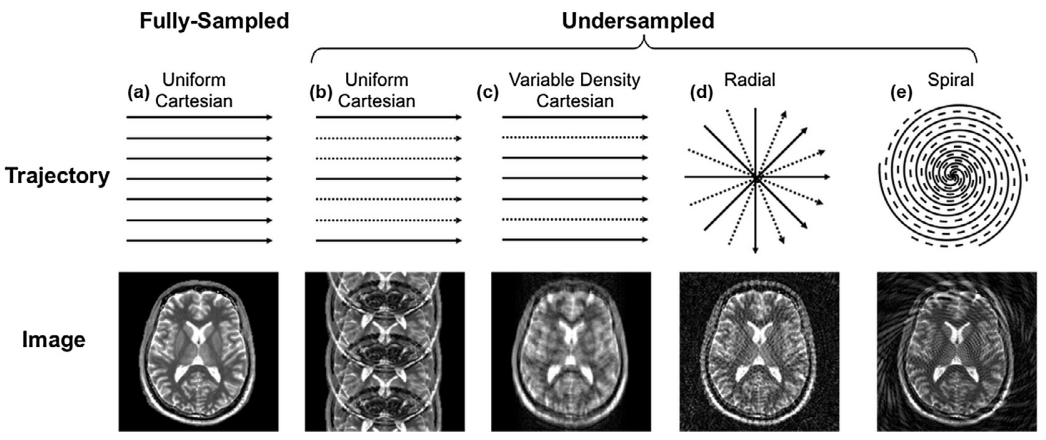
\includegraphics[width=\linewidth]{ExamplesSubsampling.png} 
	\caption{Examples of different subsampled k-space trajectories and their associated aliasing artifacts (omitted/zeroed data represented by dashed lines) taken from~\cite{AdvancesPI}.}
	\label{fig:ExamplesSubsampling}
\end{figure}

\subsubsection{Parallel Imaging}
Parallel imaging (PI) is a robust method for accelerating the acquisition of MRI data by subsampling the k-space data using an array of receiver coils. One of several PI algorithms can then be used to reconstruct artifact-free images from either the aliased images (SENSE-type reconstruction) or from the under-sampled data (GRAPPA-type reconstruction). PI requires special hardware known as phased array coils that 
%are now supplied with nearly every modern clinical scanner. Phased arrays 
contain multiple independent receiver channels. Each coil element is most sensitive to the magnetization closest to it and less sensitive to magnetization further away. 
%The spatial sensitivity can be visualized as the coil’s sensitivity profile (Fig. 3). Note that in these maps, the coil sensitivity falls off rapidly with increasing distance from the coil. 
Individually, each coil has high local signal-to-noise ratio (SNR) but inhomogeneous coverage. To expand the FOV while maintaining high SNR, several coils are organized in an array. The images from each channel are usually combined into a single image with relatively homogeneous intensity by taking e.g. a root sum-of-squares combination.
% or using more advanced methods that preserve SNR [14]. Dedicated surface coil arrays are provided for different parts of the body. Coil arrays can have up to 32 [15,16], 64 [17], or 96 [18] channels for brain imaging or 128 channels for cardiac imaging [19], although most high-count arrays are still in research development.
%Intuitively, every coil can be used to generate a unique view of the object, which provides additional spatial information that can partially replace gradient encoding to reduce scan time. Each coil detects signals from the object weighted by the coil’s sensitivity profile. This weighting can be modeled as a multiplication of the coil sensitivity profile and the magnetization. The use of a coil with an inhomogeneous sensitivity also affects k-space. Multiplication in the image domain is equivalent to convolution in the frequency domain. Therefore, in k-space the Fourier Transform of the image is convolved with the spectrum of each coil’s sensitivity profile.
Theoretically, the maximum acceleration factor is limited by the number of coils
%, as will be explained in the SENSE section. 
,thus, for PI to be successful, each coil must have a unique sensitivity variation along the direction that is accelerated. For example, an array with four coils arranged in a line may be able to attain a maximum R = 4 along one direction, but no acceleration would be possible in the perpendicular direction~\cite{AdvancesPI}.\\
As mentioned before, PI techniques fall into one of two classes, depending on whether aliased pixels are separated in the image domain (SENSE) or missing phase encoding lines are reconstructed in k-space (GRAPPA). Sensitivity encoding (SENSE)~\cite{SENSE1} is a PI technique which unfolds superimposed pixels in the image domain. For Cartesian k-space sampling with a uniform acceleration factor of R = 3 and a receiver array with four coils the undersampling reduces the FOV threefold, such that three pixels from the fully-sampled image fold onto the same pixel in the aliased image. SENSE uses prior knowledge of the coil sensitivity profiles to separate folded pixels and recover the full FOV image. 
%The first step in the SENSE reconstruction is to form a sensitivity matrix S for a given pixel in the aliased image. This matrix has size nc  np, where nC is the number of coils and np is the number of aliased pixels, which is equal to the acceleration factor. Let the signal at location ðx; yÞ in the aliased dataset received by coil j be denoted I aliased j ðx; yÞ. It can be expressed as the sum of three pixels in the full FOV image that have been weighted by their coil sensitivities and are separated by distance FOV=3.
If the acceleration factor exceeds the number of coils, then the
SENSE 
%equations will not be invertible. 
algortihm will not be able to recover an un-aliased image.
In practice, the largest achievable acceleration factor is usually smaller than the theoretical limit because coil sensitivities overlap and are not orthogonal~\cite{AdvancesPI}.\\
One common feature of PI is the amplification of noise in the reconstructed image, though with varying degrees:
\begin{equation} \label{eq:SNR-SENSE}
	SNR_{SENSE}(x,y) = \frac{SNR_{full}(x,y)}{\sqrt{R} \cdot g(x,y)},
\end{equation}
where the geometry factor $g(x,y)$ describes the spatial pattern of noise enhancement, $SNR_{SENSE}(x,y)$ the SNR in the reconstructed SENSE image and $SNR_{full}(x,y)$ the SNR of the fully sampled image. In addition to the g-factor losses, which depend on variables like number of coils, array configuration, etc., the SNR decreases with the square root of the acceleration factor $R$, which is known as Fourier averaging.\\
%It depends on many variables, including the number of coils, array configuration, coil loading, and scan plane orientation. The signal-to-noise ratio (SNR) in the reconstructed SENSE image is related to that of the fully sampled image according to
While SENSE unfolds aliased signals in the image domain, generalized partially parallel acquisitions (GRAPPA)~\cite{GRAPPA} synthesizes missing data points directly in k-space. 
%As described above and shown in Fig. 3, collecting data with multiple inhomogeneous receiver coils weights the magnetization by each coil’s sensitivity profile. In k-space
There, the use of inhomogeneous receiver coils effectively spreads information from one k-space point to nearby k-space points. GRAPPA exploits these k-space redundancies across coils to reconstruct missing k-space data using neighboring acquired points. A single missing k-space data point (target point) is synthesized as a linear combination of acquired neighboring k-space points (source points) with the spatial arrangement of source and target points being called GRAPPA kernel. Each acquired source point is multiplied by a coefficient (GRAPPA weight) and the results are added to estimate the target point. A single target point for one coil is reconstructed using source points from all other coils. For Cartesian sampling, the weights are shift invariant to a first approximation, so the same GRAPPA weights can be applied throughout k-space. The reconstruction can be described as convolving or sliding the GRAPPA kernel throughout k-space.
%; as the kernel moves from point to point, the weights are multiplied by the kernel source points to reconstruct the kernel’s target points (Fig. 7). A typical kernel may consist of six source points from each coil, with three in the readout direction and two in the phase encoding direction, centered around a target point. Including more source points tends to improve the reconstruction quality but may require additional calibration data, as discussed below.
While SENSE uses additional information in the form of coil sensitivity profiles to unfold aliased pixels, GRAPPA requires extra data to estimate the weights. GRAPPA is considered to be autocalibrating because several additional phase encoding lines, called the auto-calibration signal (ACS), are collected near the k-space origin for calculating the weights. 
%The GRAPPA kernel is moved to every possible position within the ACS to accumulate many instances where the source points and target points are both known. Then the GRAPPA equation can be inverted to solve for the unknown weights.
The SNR of images reconstructed using GRAPPA is also reduced according to Equation~\ref{eq:SNR-SENSE}, however, because GRAPPA does not require an explicit estimate of the coil sensitivities, it tends to be more robust than SENSE to inconsistencies between the calibration and undersampled data~\cite{AdvancesPI}.\\
SENSE and GRAPPA can be combined in what is called iterative self-consistent parallel imaging (SPIRiT)~\cite{SPIRiT}. Like GRAPPA k-space kernels are used to recover missing information by exploiting correlations between neighboring k-space points, though the reconstruction is framed as an inverse problem similar to SENSE. Regardless of the original sampling trajectory, SPIRiT outputs a Cartesian k-space. The reconstruction is typically initialized with the undersampled zero-filled k-space and is solved iteratively. 
%as an optimization problem. 
%On each iteration, the algorithm moves toward a solution that 
The algorithm 
minimizes and balances the errors of two terms: calibration consistency and data consistency. The first is calculated using a so-called SPIRiT kernel in the k-space similar to GRAPPA, while the second term enforces consistency with the undersampled data as the difference between the reconstructed data and acquired data should be zero at the originally sampled positions. Thus reconstruction should only recover missing k-space points without changing the known data points~\cite{AdvancesPI}.%\\
ESPIRiT~\cite{ESPIRiT} is an extension of SPIRiT that uses k-space kernel operations to derive a set of eigenvector maps that behave like coil sensitivities, which can be incorporated in a generalized SENSE reconstruction. This requires calibration data from the fully sampled region at the center of k-space. 
%A k-space kernel is moved to each possible position within this region, and each instance of the kernel is reshaped to populate a row in a special matrix. Many of the singular values of this matrix are small or close to zero, meaning that it has a null space. The existence of a null space implies that neighboring k-space points in the multichannel data are correlated. Missing k-space data are reconstructed by recognizing that this relationship should be true not only over the calibration region but also over the entire k-space.
Unlike SENSE and GRAPPA, SPIRiT reconstructs images iteratively and can require long computation times which can be addressed by using e.g. parallelized GPUs~\cite{AdvancesPI}.

\subsubsection{Compressed Sensing}
The idea behind compressed sensing (CS) is that sparse or compressible signals can be acquired in an efficient way by applying compression already in the data acquisition process. According to CS theory, sparse or compressible signals can be recovered from fewer samples than required by the Shannon-Nyquist sampling theorem~\cite{CS-MRI}. This is achieved by applying an appropriate sampling scheme and reconstruction that employs signal sparsity to recover the signal. MRI fulfills two important requirements for the application of CS: medical imaging is naturally compressible by sparse coding and MRI scanners acquire samples of the encoded image in spatial frequency, rather than direct pixel values. CS emerged as an abstract mathematical idea that if one measures a relatively small number of random linear combinations of the signal values the signal can be reconstructed with good accuracy from these few measurements by a non-linear procedure due to the underlying signal being compressible.
% – much smaller than the number of signal samples nominally defining it. However, because the underlying signal is compressible, the nominal number of signal samples is a gross over-estimate of the effective number of degrees of freedom of the signal. As a result, the signal can be reconstructed with good accuracy from relatively few measurements by a non-linear procedure. 
In MRI, the sampled linear combinations are the individual Fourier coefficients (k-space samples) and CS is able to make accurate reconstructions from a small subset of k-space, rather than an entire k-space grid~\cite{CS-MRI}. It should be noted that unlike PI approaches, the k-space is incoherently sampled; thus, noise-like artefacts appear in the image when a direct inverse Fourier transform is performed. To remove the artefacts caused by the undersampling, iterative reconstruction is used. There are a number of sparsifying transforms that can be used for CS such as wavelets, which are very common, and total variation, which enforces the sparsity of the image gradients. The advantages of total variation include its simplicity, rotation invariance, and capability of preserving edges and providing good image quality~\cite{PulseSequences}. There are also several methods combining CS and PI trying to achieve higher acceleration factors~\cite{PI+CS, PI+CS2}.
%, but with the addition of regularization that enforces sparsity by penalizing coefficients in some domain (e.g. Wavelet, finite difference) with a $L_1$-norm

\subsubsection{Deep Learning Based Subsampling} \label{SubSubSec:DeepLearningBasedSubsampling}
There are also approaches for learning new subsampling strategies in a data-driven manner (pruning unimportant k-space frequencies)~\cite{MRISubsamplingPruning} as well as deep learning based radial~\cite{DeepMRIReconstructionRadialSubsampling} and non-Cartesian~\cite{DeepMRIReconstructionSubsampling} subsampling for MRI acceleration.


\subsection{Motion-Compensated Image Reconstruction} \label{SubSec:Motion-CompensatedReconstruction}
Patient motion during acquisition is one of the major impediments of high-quality MRI scans. This is especially true for thoracic and abdominal imaging, as organs move during breathing. Steps can be taken during or after the reconstruction to mitigate motion artifacts.

\subsubsection{Intraview and Interview Motion} \label{SubSubSec:IntraviewandInterviewMotion}
Due to the long acquisition times, motion is one of the major extrinsic factors influencing MR image quality. Patient and physiological motion induces aliasing along the phase-encoding direction and/or blurring of the image content~\cite{Kuestner2022}.
%, where the appearance depends on the imaging trajectory.
This motion can induce several consequences on MR signal formation. Intraview and interview motion have to be distinguished between: motion is intraview when occurring during individual MR experiments (between RF excitation and echo formation), whereas motion is interview when occurring between individual MR experiments. Whenever the period of motion is slow compared to the period of MR acquisition 
%defined by the repetition time 
$TR$, the assumption can be made that motion is interview. This is often a reasonable assumption when considering pseudo-periodic motion induced by respiration, and also possibly by cardiac contraction, which are the two common sources of motion in cardiac and abdominal imaging (typically, the adult respiratory period is about 4 to 5~s, and $TR \approx 10$~ms for fast imaging). Interview motion results in spatial encoding inconsistencies, and thus in image deterioration which can take complex forms (blurring/ghosting artifacts) as acquisition is performed in a Fourier space. Several strategies can be employed in order to handle patient motion better. Patient cooperation is the most commonly used method. However, breath-holds cannot last much longer than 20~s and physiological drifts cannot be completely avoided. This leads to a limitation on the time-period of signal recording and thus SNR. Moreover, the position of organs in successive breath-holds may not be reproducible. Synchronization techniques are well-established and systematically used in clinical protocols, but they require a high-level of motion reproducibility. This is often a limiting factor considering heart rate variability (whether in free breathing or during a breathhold), and respiratory variability in terms of amplitude and frequency~\cite{GRICS}. 
%This is why alternative techniques have been put forward with the aim of inverting the process of spatial encoding of moving structures that underlies artifacts. While it is possible to correct for motion prospectively, by modulating the magnetic field gradients and RF fields in order to cancel the effect of motion in the Bloch equations, the method is limited to correcting of, at best, affine motion, due to magnetic field gradient systems being linear. 

\subsubsection{Reconstruction Pipelines} \label{SubSubSec:ReconstructionPipelines}
Motion-resolved data acquisition is usually accelerated by PI or CS techniques yielding subsampled k-space data. In order to reconstruct aliasing-free images, these methods rely on reconstruction schemes that incorporate sparsity or low-rank constraints to solve the ill-posed problem~\cite{CS-MRI,ParallelMRI,LowRank+SparseMRI}. Fixed sparsity assumptions in CS are often too restrictive and incapable of fully modeling spatio-temporal dynamics~\cite{Kuestner2022}. 
%Careful fine-tuning between regularization and data consistency is required and especially in highly subsampled cases residual aliasing may remain in the image (under-regularization) or staircasing and blurring artifacts can occur (over-regularization) which affect the image registration. 
After reconstruction, non-rigid motion fields can be estimated in image space from reconstructed images by solving a registration problem. A particular interest and challenge lies in the derivation of reliable motion fields which capture the spatio-temporal non-rigid deformations, such as respiratory or cardiac movement. Instead of performing these two steps sequentially, motion-compensated image reconstruction schemes like \emph{GRICS}~\cite{GRICS} integrate both motion field estimation and motion correction into the reconstruction process. These methods require reliable motion-resolved images from which the motion fields can be estimated. Motion field estimation can be controlled or supported by external motion surrogate signals, initial motion field estimates, from motion-aliased images or low-frequency image contents. Moreover, spatio-temporal redundancies can be exploited to achieve an aliasing-free image. While these methods have been proven to be more robust against registration errors, they can require a significantly increased computational demand and/or limit imaging acceleration~\cite{Kuestner2022}.\\
There are two major parts of a motion-compensated reconstruction pipeline: a non-rigid registration model to reliably estimate the motion fields between frames and an unrolled reconstruction model that reconstructs the motion-corrected frames. Both of these can use either conventional iterative algorithms like in GRICS~\cite{GRICS} or neural networks that learn the given task~\cite{Kuestner2022}.


\section{Image Transformations and Registration} \label{Sec:ImageTransformationsAndRegistration}
In this chapter, a brief overview over the different kinds of image transformations is given, followed by an introduction into the challenges of image registration.\\
The goal of image registration is to compute a transformation that aligns two images - moving and fixed. This transformation is then applied to the moving image to create an warped image that more closely resembles the fixed image. But first, the different kinds of image transformations must be discussed.

\subsection{Image Transformations} \label{SubSec:ImageTransformations}
In medical image registration, there are three basic transformation types that are typically applied: rigid, affine and non-linear(deformable)~\cite{Strittmatter2023}.

\subsubsection{Rigid Transformations}
Rigid transformations are linear and global transformations that affect the whole image. As these are global operations, one can express them as matrix and vector operations. A rigid transformation includes translation and rotation and can be represented by:
\begin{equation}
	\mathbf{T}_{rigid} (x) = \mathbf{R} \cdot \overrightarrow{p} + \overrightarrow{t},
\end{equation}
with $\mathbf{R}$ being the rotation matrix, $\overrightarrow{p}$ a point in the image and $\overrightarrow{t}$ the translation vector.  For 3D images, the rotation matrix and the translation vector require three parameters each. Thus, six parameters have to be calculated for a rigid transformation for 3D images~\cite{Strittmatter2023}.

\subsubsection{Affine Transformations}
Affine transformations are also linear and global transformations, however they include translation, rotation, scaling and shearing. Matrix multiplication can be used to merge all of these individual transformations into a single matrix:
\begin{align}
	\overrightarrow{p}' 	&= \mathbf{R} \cdot \mathbf{S} \cdot \mathbf{t} \cdot  \overrightarrow{p}	\\
	&= 
	\begin{bmatrix}
		\cos(\theta) & -\sin(\theta) & 0\\
		\sin(\theta) & \cos(\theta) & 0\\
		0 & 0 & 1
	\end{bmatrix}
	\cdot 
	\begin{bmatrix}
		s & 0 & 0\\
		0 & s & 0\\
		0 & 0 & 1
	\end{bmatrix}
	\cdot 
	\begin{bmatrix}
		1 & 0 & t_x\\
		0 & 1 & t_y\\
		0 & 0 & 1
	\end{bmatrix}
	\cdot
	\begin{bmatrix}
		x\\
		y\\
		1
	\end{bmatrix}
	\\
	&=
	\begin{bmatrix}
		s \cdot \cos(\theta) & -s \cdot \sin(\theta) & t_x\\
		s \cdot \sin(\theta) & s \cdot \cos(\theta) & t_y\\
		0 & 0 & 1
	\end{bmatrix}
	\cdot
	\begin{bmatrix}
		x\\
		y\\
		1
	\end{bmatrix} =
	\begin{bmatrix}
		x'\\
		y'\\
		1
	\end{bmatrix} ,
\end{align}
with $\theta$ being the angle of the rotation for the rotation matric $\mathbf{R}$, $s$ the scaling factor for the scaling matrix $\mathbf{S}$ as well as $t_x$ and $t_y$ being the translations in x- and y-direction. This can be further generalized as a single matrix multiplication:
\begin{equation}
	\overrightarrow{p}' = \mathbf{T}_{affine} \cdot  \overrightarrow{p} = 
	\begin{bmatrix}
		a_{11} & a_{12} & a_{13}\\
		a_{21} & a_{22} & a_{23}\\
		0 & 0 & 1
	\end{bmatrix}
	\cdot
	\begin{bmatrix}
		x\\
		y\\
		1
	\end{bmatrix}
	 = 
	 \begin{bmatrix}
		x'\\
		y'\\
		1
	\end{bmatrix},
\end{equation}
with $\mathbf{T}_{affine}$ being the general affine transformation matrix~\cite{Strittmatter2023}.

\subsubsection{Non-Linear Transformations}
Non-linear or deformable transformations are used to model local deformations in images that rigid and affine transformations cannot capture as these transformations are capable of locally warping the image. Non-linear transformations include radial basis functions, physical continuum models, and large deformation models like diffeomorphisms. These transformations are complex and do not preserve straightness or parallelism:
\begin{equation}
	\mathbf{T}_{deformable} (x) = x + \phi (x),
\end{equation}
with $\phi$ being the deformation or displacement field. Deformable image registration is an ill-posed problem, often requiring regularization to ensure a smooth and plausible displacement field~\cite{Strittmatter2023}.

\subsection{Image Registration} \label{SubSec:ImageRegistration}
Image registration is a challenging, yet important task for image processing. In the field of medical image analysis, image registration remains one of the main research topics and challenges. This task consists of transforming a moving image to match a fixed image~\cite{NiftiReg}. 
%The most active area of research is non-rigid registration, in which attempts are made to locally warp one image into correspondence with another. Example problems are matching 3D MRI scans of two different patients, or two scans of the same patient before and after surgery. 
%It can be described as the process of transforming different image datasets into one coordinate system with matched imaging contents~\cite{Haskins2020}. 
In the medical field this can be used for clinical applications such as disease diagnosis and monitoring, image-guided treatment delivery, and post-operative assessment. Medical image registration is typically used to pre-process data for tasks like object detection (for e.g. tumor growth monitoring) and segmentation (for e.g. organ atlas creation).
%where variation in spatial resolution is common between modalities like CT and MRI and patients. 
Thus the performance of these methods is dependent on the quality of image registration~\cite{Chen2020}. \\
Medical image registration was historically done manually by clinicians, however, registration tasks are often challenging and the quality of manual alignments is dependent on the expertise of the user. These manual registrations are thus not only time consuming, but also hardly reproducible leading to high interobserver-variability. While the need for automatic registration is very much apparent, the computational cost of traditional registration algorithms prohibited their usage for a long time. 
%but this task remained hard to solve for a long time, requiring a lot of computational power and time for computer algorithms to solve the problem. While neural networks also require a lot of computational power and time to train, they promise fast execution after training. 
With the rise of deep learning, neural network gained popularity and now provide an alternative to conventional algorithms and manual registration that is fast and computationally efficient during execution~\cite{Haskins2020}. However, it should be noted that these networks still need a lot of data and computational power to be trained.\\
%We will discuss these new approaches in the next section, but first we need to formally define our problem.\\
In pair-wise image registration two images, called moving ($M$) and fixed ($F$), are to be aligned with a spatial transformation T. As discussed before there are three types of transformations: rigid, affine, and non-linear (deformable). While the latter is the most difficult to compute these are also the transformations most likely encountered in clinical practice
%as it can be utilized to fuse information from different modalities such as MRI and CT
~\cite{Zou2022}. Additionally, deformable image registration can also be
utilized for various computer-assisted interventions like biopsy~\cite{Tam2016} and (MRI-guided) radiotherapy~\cite{Chen2017, Rigaud2019}. This can be described as an optimization problem:
\begin{equation}
	T' = \arg\max S(F, T(M)),
\end{equation}
where $T'$ is the best transformation maximizing the similarity $S$ between the two images. This process can be done iteratively, continuously improving the estimates for the desired T, such that the defined similarity in the cost function is maximized~\cite{Chen2020}. Intuitively, deformable image registration is an ill-posed problem making it fundamentally different from other computer vision tasks such as object localization, segmentation or classification. Given two images, deformable image registration aims to find a spatial transformation that warps the moving image to match the fixed image as closely as possible. However, there is no ground-truth available for the desired deformation field and without enforcing any constraints on the properties of the spatial transformation, the resulting cost function is ill-conditioned and highly non-convex. In order to address the latter and ensure tractability, all image registration algorithms regularize the estimated deformation field, based on some prior assumptions on the properties of the underlying unknown deformation~\cite{Chen2020}.\\
%\\Transformations can be categorized as rigid, affine, and deformable. A rigid transformation consists of rotation and translation; an affine transformation includes translations, rotations, scaling, and sheering; the two kinds of transformations are described as a 2D single matrix. Unlike rigid and affine transformation, deformable transformation is a high-dimension problem that we need to formulate by a 3D matrix for 2D deformable registration i.e., a so-called deformation field. While rigid and affine registration algorithms have already achieved good performance in many applications, deformable registration is still a challenging task due to its intrinsic complexity, particularly when the deformation is large. \\
Many methods have been proposed for medical image registration to deal with the complex challenges of this task. Popular conventional registration methods include optical flow~\cite{Yang2008}, demons~\cite{Vercauteren2009} and many more. However, most of these still lack accuracy and computation speed, which makes newer deep learning approaches all the more interesting~\cite{Fu2020}.


\section{Deep Learning} \label{Sec:DeepLearning}
Deep learning, and neural networks in general, have seen a significant rise in usage over the last couple of years due to many breakthroughs in areas of image recognition, segmentation and also registration. After discussing different network architectures, specific use-cases for image registration are discussed and a brief overview of network training and testing (including evaluation metrics) is given.

\subsection{Deep Learning Architectures} \label{SubSec:DeepLearningArchitectures}
Neural networks, despite the theoretical foundations being around for decades, have seen a drastic rise in popularity over the last few years as constraints on computational power and data size have been alleviated. Especially deep neural networks, which are often summarized under the term deep learning (DL). Recent years have witnessed an almost exponential growth in the development and use of DL algorithms, sustained thus far by rapid improvements in computational hardware (e.g. GPUs). Consequently, clinical applications requiring image classification, segmentation, registration, or object detection/localization, have witnessed significant improvements in algorithmic performance, in terms of accuracy and/or efficiency~\cite{Chen2020}. The following network architecture are widely used for different tasks including medical image registration.

\subsubsection{Convolutional Neural Networks} \label{SubSubSec:CNNs}
Convolutional neural networks (CNNs) are a type of deep neural networks with regularized multilayer perceptron, which are mainly used for image processing. CNNs use convolution operations instead of general matrix multiplications in typical neural networks. These convolutional filters make CNNs very suitable for visual signal processing. Because of their excellent feature extraction ability, CNNs are some of the most successful models for image analysis. Different variants of CNN have been proposed and have achieved the-state-of-art performances in various image processing tasks. A typical CNN usually consists of multiple convolutional layers, max pooling layers, batch normalization layers, sometimes dropout layers, a sigmoid or softmax layer. In each convolutional layer, multiple channels of feature maps are extracted by sliding trainable convolutional kernels across the input feature maps. Hierarchical features with high-level abstraction are extracted using multiple convolutional layers. These feature maps usually go through multiple fully connected layer before reaching the final decision layer. Max pooling layers are often used to reduce the image sizes and to promote spatial invariance of the network. Batch normalization is used to reduce internal covariate shift among the training samples. Weight regularization and dropout layers are used to alleviate data overfitting~\cite{Fu2020}. The loss function is often defined as the difference between the predicted and the target output. CNNs are usually trained by minimizing the loss via gradient back propagation using optimization methods like Adam~\cite{Adam}. % lieber stochastical gradient nehmen?
% Convolutions and Deconvolutions genauer erklären?!

\subsubsection{U-Net} \label{SubSubSec:U-Net}
The U-Net~\cite{U-Net} architecture is an extension of the usual CNN structure often used for image segmentation, however, it can also be applied to image registration tasks. It adopts symmetrical contractive and expansive paths with skip connections between them as seen in Figure~\ref{fig:U-NetArchitecture}. The encoding blocks on the left extract important features from the image using convolution layers and max pooling, which are then stored in the latent space in the middle. From there it is reconstructed using upsampling and (de-)convolutions in the decoding blocks on the right. Additionally, skip connections are used to improve the spatial resolution of the segmentation. This architecture allows effective feature learning from a small number of training datasets~\cite{Fu2020}. 

\begin{figure}[h] %tpb
	\centering
	\graphicspath{{images/}{\main/images/}}
	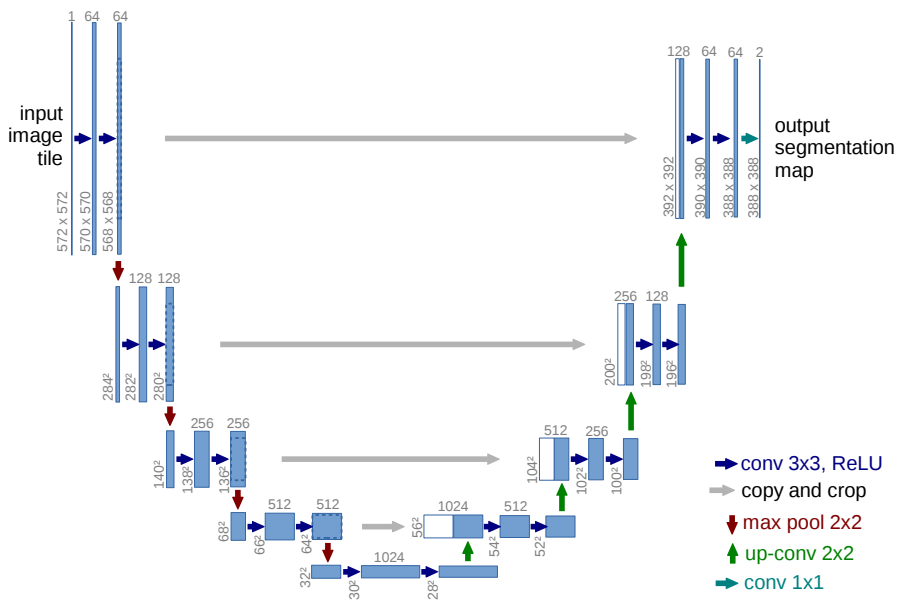
\includegraphics[width=.75\linewidth]{U-NetArchitecture.png} 
	\caption{U-Net architecture taken from~\cite{U-Net} with an contractive path on the left and an expansive path on the right.}
	\label{fig:U-NetArchitecture}
\end{figure}

\subsubsection{Autoencoders} \label{SubSubSec:Autoencoders}
An autoencoder (AE) is a type of CNNs that learns to reconstruct an image from its input without supervision. AEs usually consists of an encoder which extracts the input features, which are stored a low-dimensional latent state space, similar to a U-Net, and a decoder which restore the original input from the latent space. To prevent an AE from learning an identity function, regularized autoencoders were invented, which can be used for e.g. denoising AEs. Variational AEs (VAEs) are generative models that learn latent representation using a variational approach, which constrains the variability of the outputs. VAEs can been used for anomaly detection and image generation~\cite{Fu2020}.

\subsubsection{Generative Adversarial Networks} \label{SubSubSec:GANs}
Generative adversarial networks (GANs) consist of two competing networks, a generator and a discriminator. The generator is trained to generate artificial data that approximate a target data distribution from a low-dimensional latent space similar to an AE. The discriminator is trained to distinguish the artificial data from actual data. The discriminator encourages the generator to predict realistic data by penalizing unrealistic predictions via learning. Therefore, the discriminative loss could be considered as a dynamic network-based loss term. The generator and discriminator both are getting better during training to reach Nash equilibrium. In medical imaging, GANs have been used to perform image synthesis for inter- or intra-modality, such as MRI to synthetic CT and vise versa. In medical image registration, GANs are usually used to either provide additional regularization or translate multi-modal registration to uni-modal registration~\cite{Fu2020}.

\subsection{Deep Learning for Image Registration} \label{SubSec:DLImageRegistration}
Recently, there has been a surge in the use of deep learning based approaches for medical image registration. Their success is largely due to their ability to perform fast inference, and the flexibility to leverage auxiliary information such as anatomical masks as part of the training process. The most effective methods, such as \emph{VoxelMorph}~\cite{Voxelmorph}, typically employ a U-Net style architecture to estimate dense spatial deformation fields. These methods require only one forward pass during inference, making them orders of magnitude faster than traditional iterative methods. Following the success of \emph{VoxelMorph}, numerous deep neural networks have been proposed for various registration tasks~\cite{Fourier-Net+}. Other approaches also utilize CNNs, AEs and GANs. Typical strategies are discussed in more detail in the following sections.

\subsubsection{Supervised Registration} \label{SubSubSec:SupervisedRegistration}
Supervised registration describes training a network with a ground truth displacement field that is either real (created by hand) or synthetic (generated via traditional iterative registration algorithms). Thus the loss can easily be calculated as the difference in the displacement fields of the network prediction and the ground truth (see Figure~\ref{fig:SupervisedRegistration} for a visual overview). These methods have achieved notable results with real displacement fields as supervision. However, this approach is very limited by the size and the diversity of the dataset. As the displacement fields are often calculated by conventional algorithms their effectiveness might be limited for difficult problems with which the traditional algorithms struggle. Fully supervised methods are widely studied and have notable results, but the generation of real or synthetic displacement fields is hard, and these displacements fields might be different from the real ground truth, which can impact the accuracy and efficiency of these kinds of methods~\cite{Zou2022}. Notable approaches include \emph{BIRNet}~\cite{BIRNet} and \emph{LAPNet}~\cite{LAPNet}, however the latter works in the k-space domain.

\begin{figure}[h] %tpb
	\centering
	\graphicspath{{images/}{\main/images/}}
	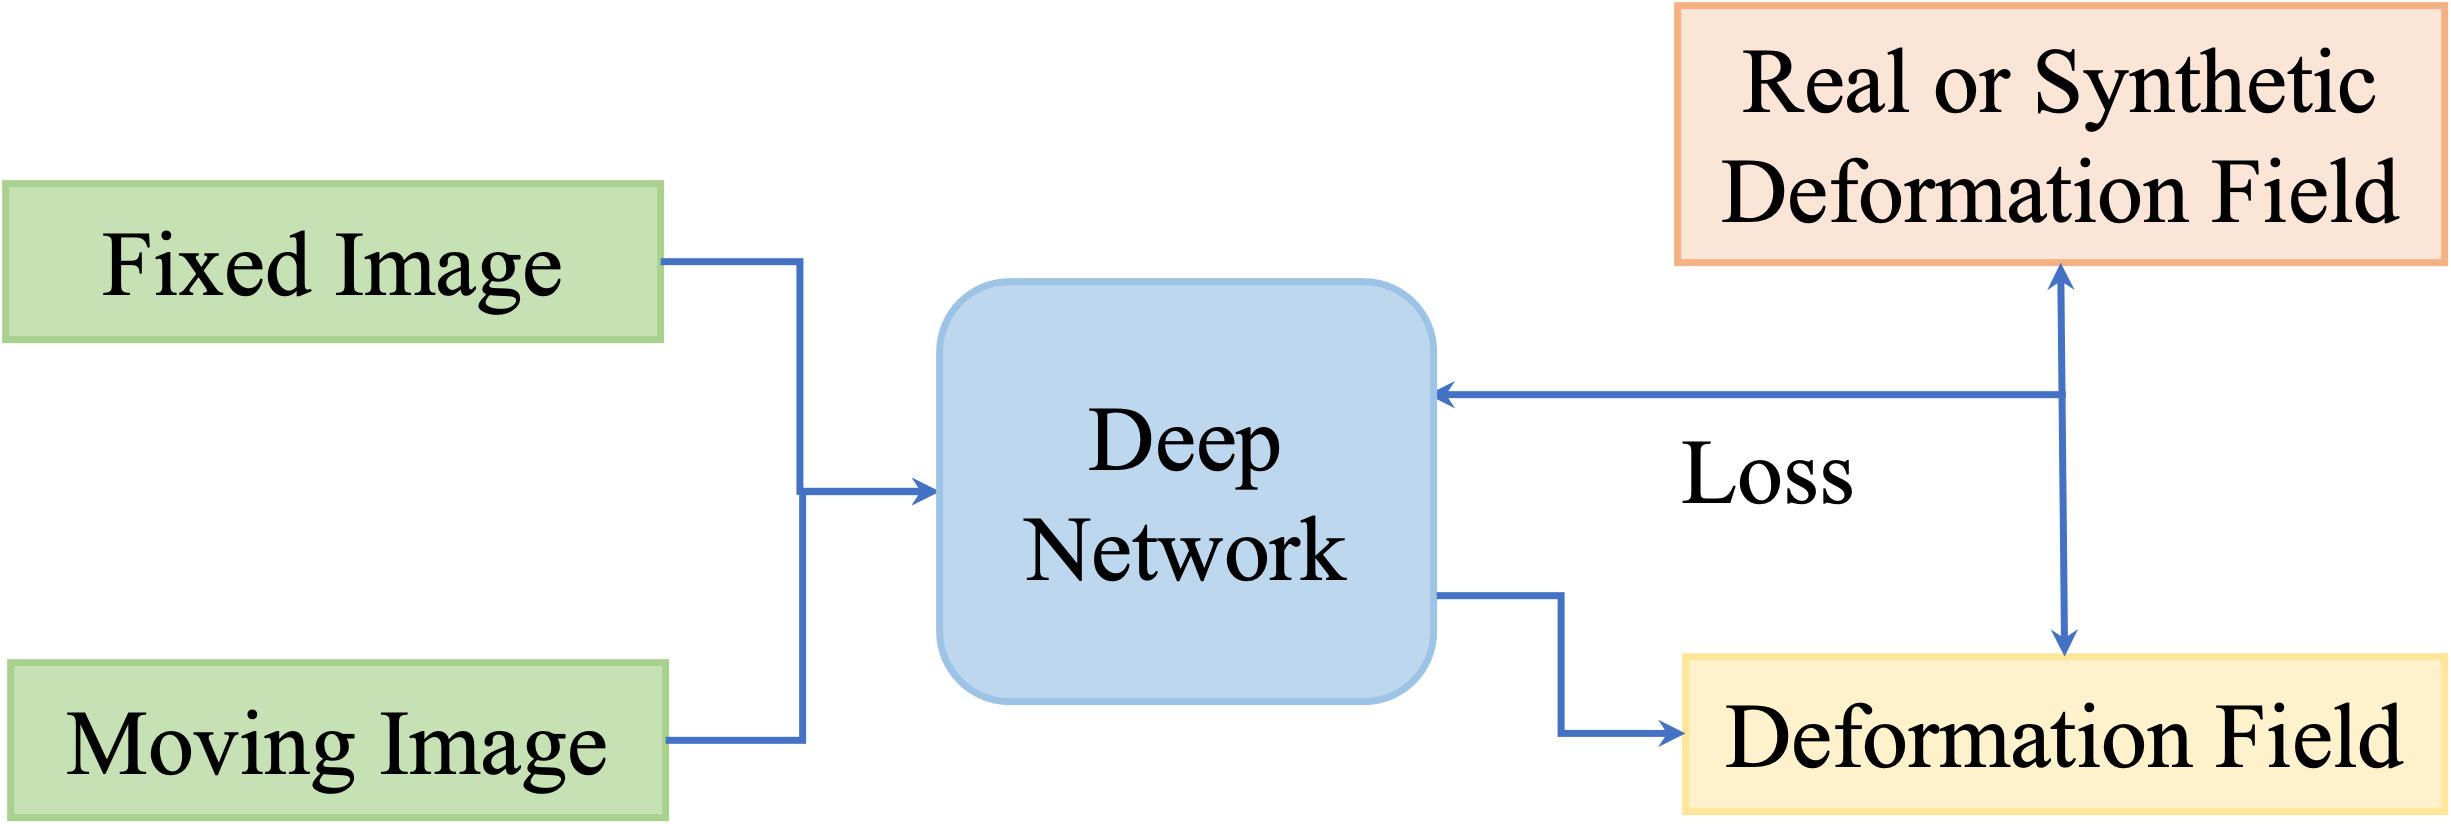
\includegraphics[width=\linewidth]{SupervisedRegistrationGraph.jpg} 
	\caption{Example graph illustrating the training process of a supervised network, taken from~\cite{Zou2022}.}
	\label{fig:SupervisedRegistration}
\end{figure}


\subsubsection{Unsupervised Registration} \label{SubSubSec:UnsupervisedRegistration}
As the preparation of the ground truth displacement field for supervised methods is inconvenient, limitations in generalizing results in different domains and various registration tasks are inevitable. Thus, unsupervised registration has a more convenient training process with paired images as inputs, but without a ground truth. Generally, unsupervised learning consists of similarity-based (see Figure~\ref{fig:UnsupervisedRegistration}) and GAN-based methods (see Figure~\ref{fig:GANRegistration}), where the loss function computes the similarity between the aligned images and the smoothness of the displacement field, rather than the difference to a ground truth~\cite{Zou2022}. Well known example are \emph{IC-Net}~\cite{IC-Net},  \emph{VoxelMorph}~\cite{Voxelmorph}, \emph{TransMorph}~\cite{TransMorph} and \emph{SYMNet}~\cite{SYM-Net}.

\begin{figure}[h] %tpb
	\centering
	\graphicspath{{images/}{\main/images/}}
	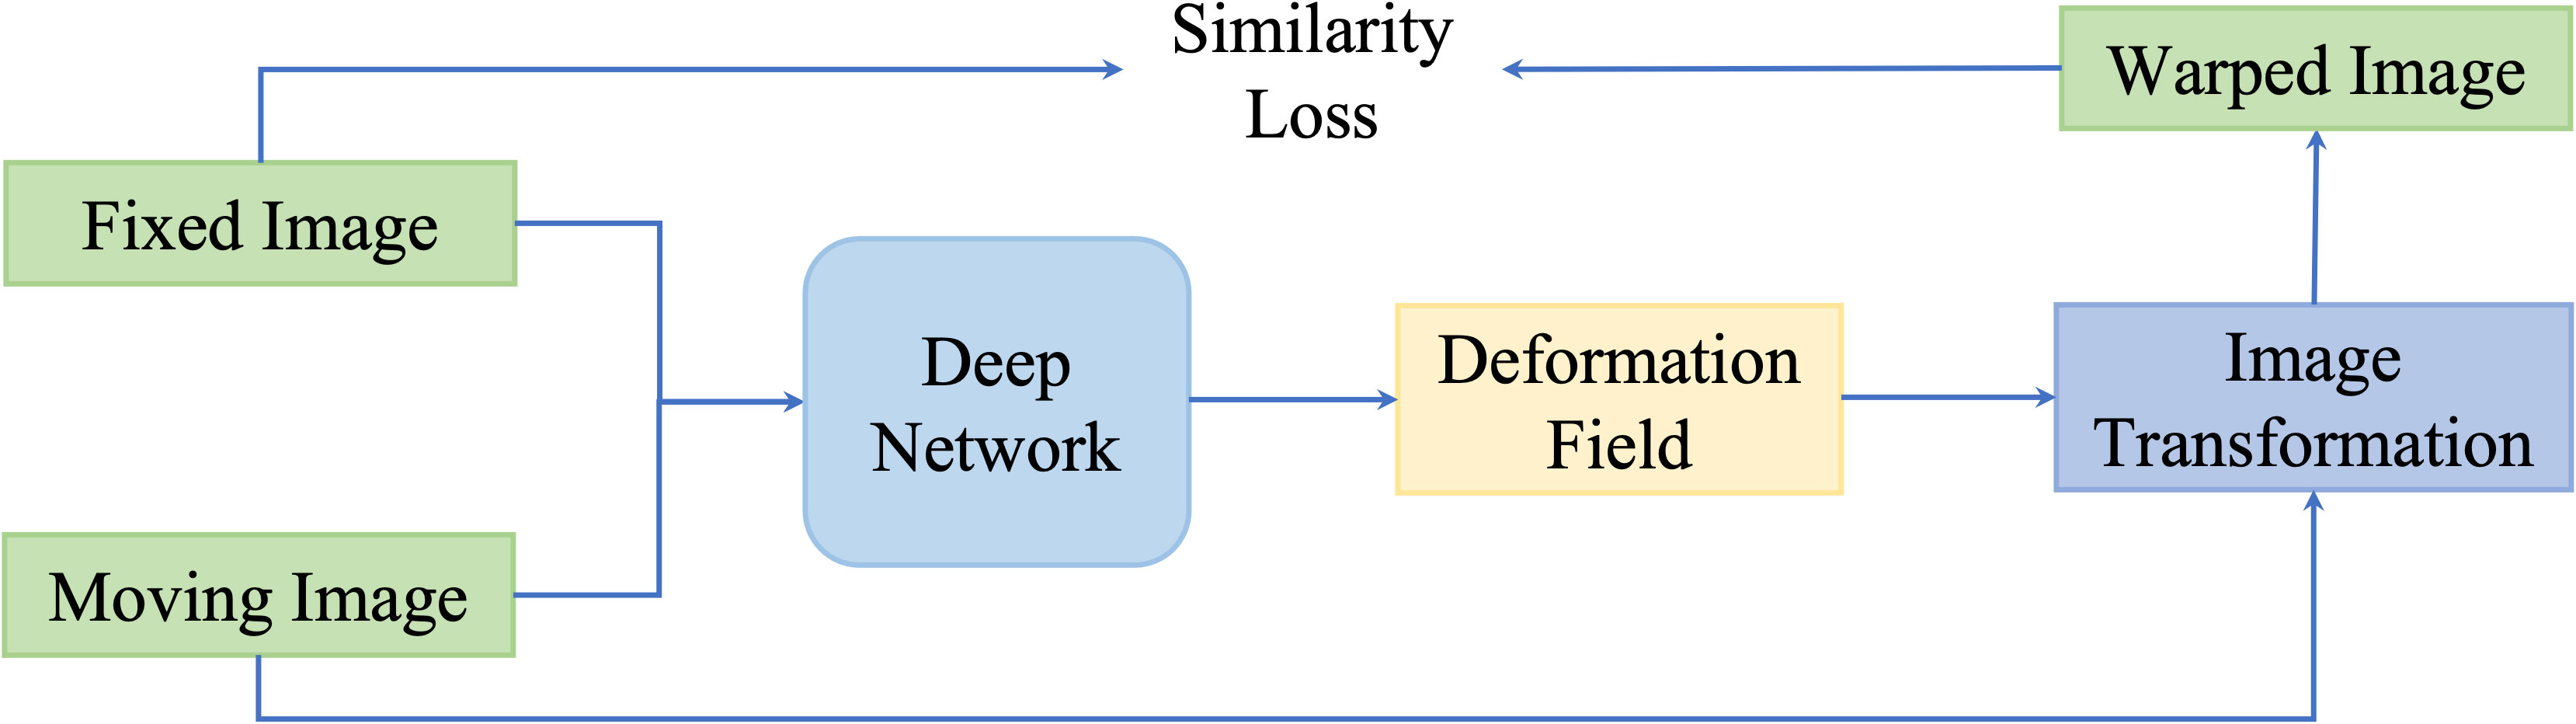
\includegraphics[width=\linewidth]{UnsupervisedRegistrationGraph.jpg} 
	\caption{Example graph illustrating the training process of an unsupervised network with only a image similarity loss, taken from~\cite{Zou2022}.}
	\label{fig:UnsupervisedRegistration}
\end{figure}

\begin{figure}[h] %tpb
	\centering
	\graphicspath{{images/}{\main/images/}}
	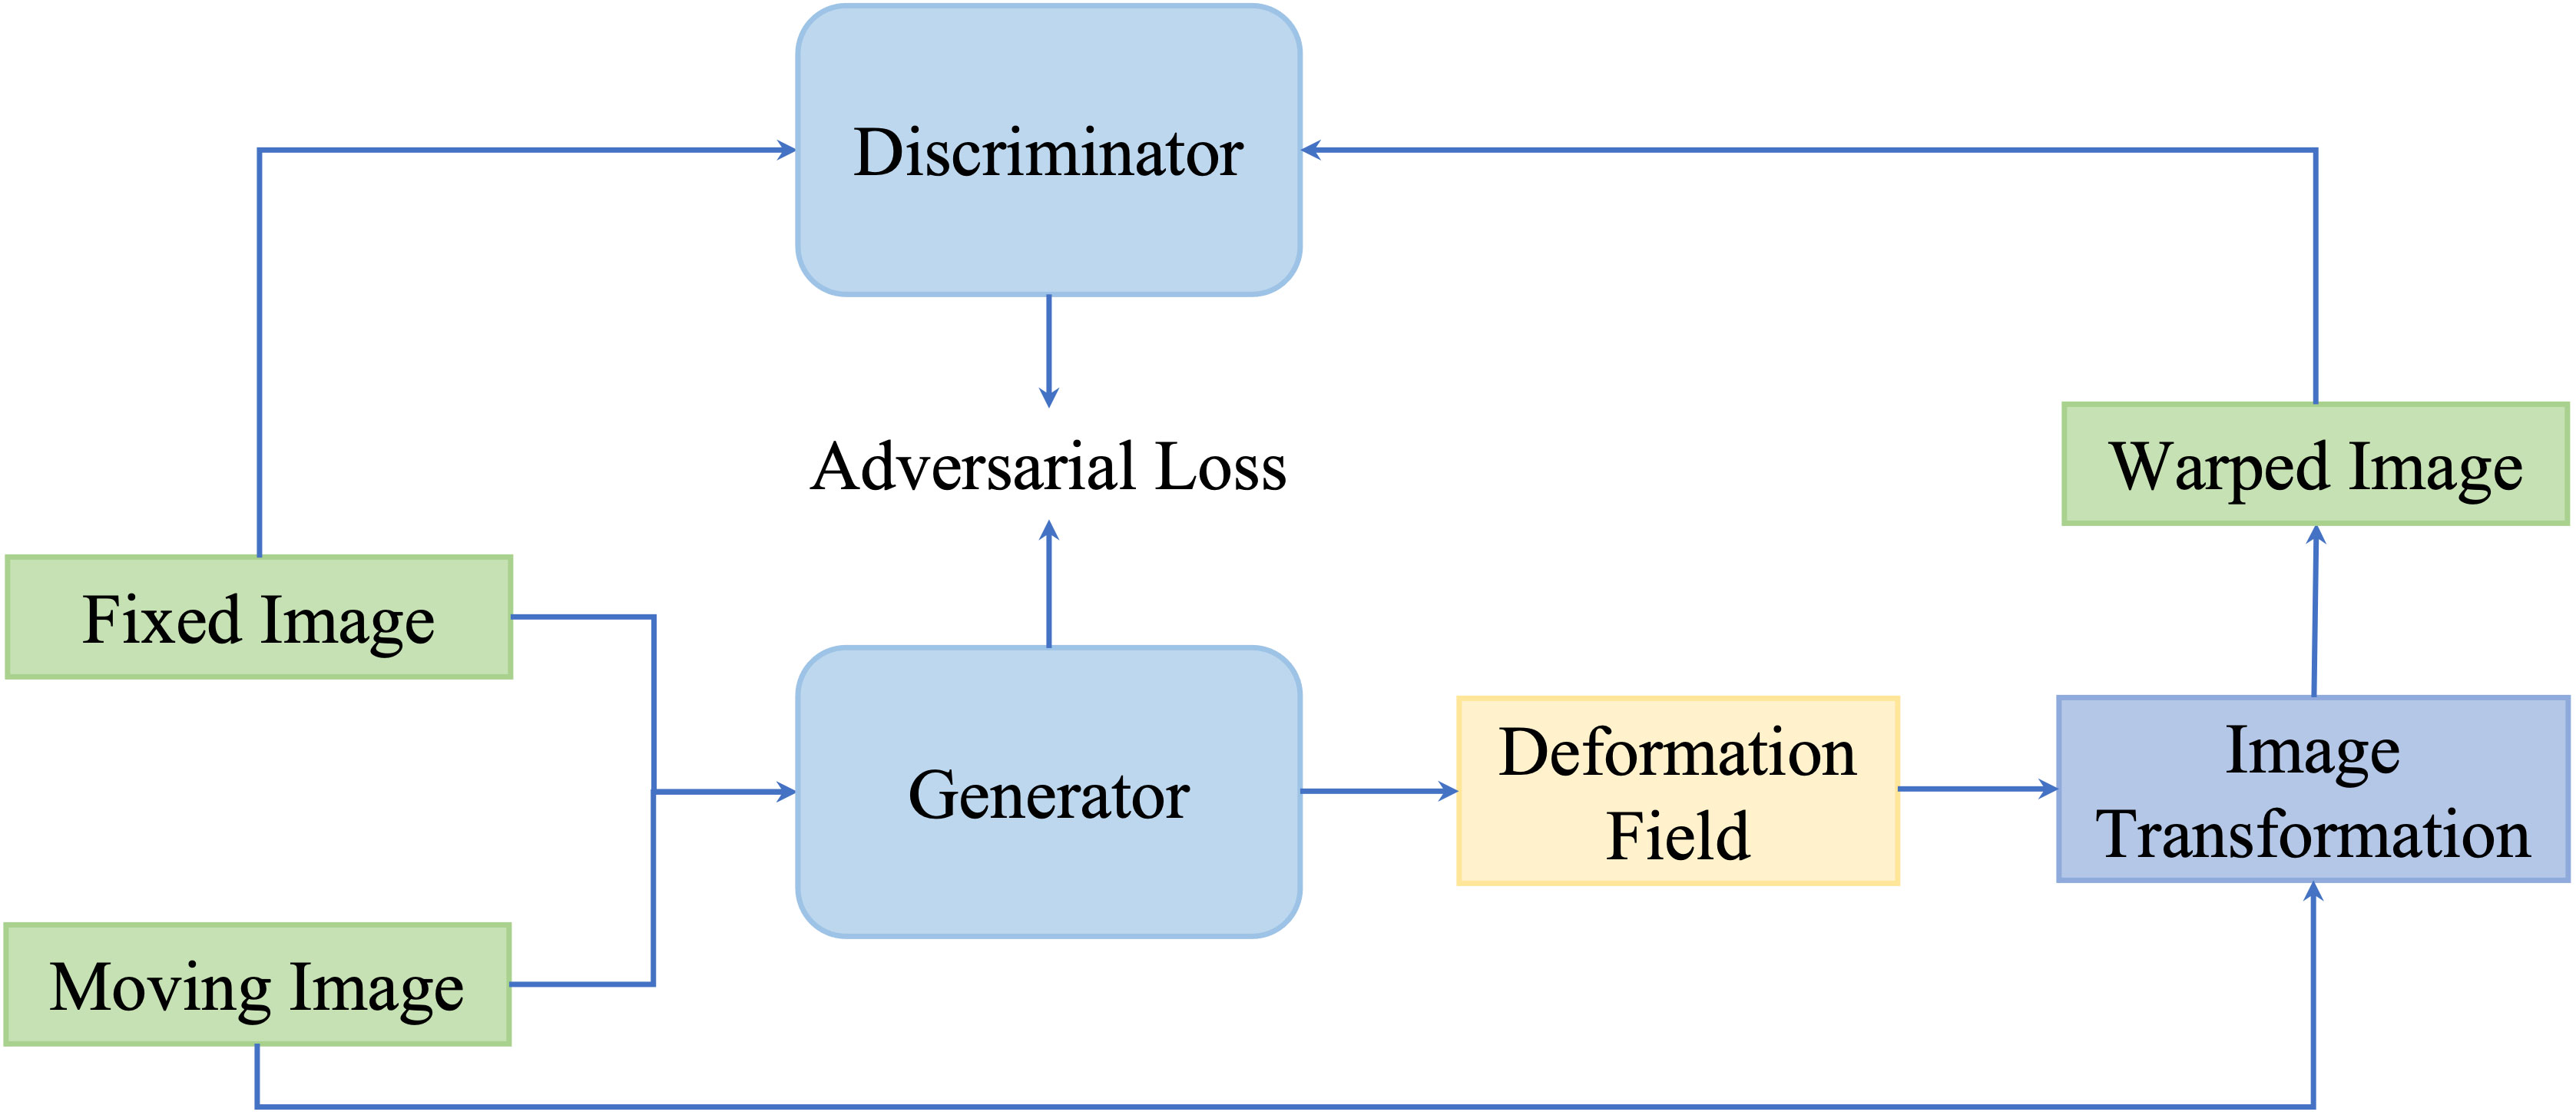
\includegraphics[width=\linewidth]{GANRegistrationGraph.jpg} 
	\caption{Example graph illustrating the training process of a GAN, taken from~\cite{Zou2022}.}
	\label{fig:GANRegistration}
\end{figure}

\subsection{Network Training and Testing} \label{SubSec:NetworkTrainingAndTesting}
In order to train any neural network, a large amount of data is needed. This data can take many forms such as videos, images, audio, text and many more. However, the total data set is usually devided into three subsets: the training, validation and testing subset. 

\subsubsection{Training and Back-Propagation}
The first subset is used for, as the name suggests, the training of the network. This if often the largest of the subsets and should include at lot of variance for the network to learn well. Neural networks in general learn by adapting their weights to perform on increasingly better at a specific task and on a specific dataset/domain. This is done in a process called back-propagation, where the loss calculated between the current output of the model, which is acquired by a simple forward pass through the network, and the desired output is propagated backwards through the model and the weights are optimized using e.g. gradiant decent or similar methods. \\
The second subsets is also used during the training, but is not learned, i.e. no back-propagation is performed. This is done to validate the networks training process and to prevent potential overfitting. Overfitting is a common problem, especially for larger networks, where the network learns every example from the training set, but no general properties as intended. To prevent this, the unseen validation data can be repeatedly used, as it is not learned by the network, to see whether the network improves on unseen data. Once it has been trained for a long time and the validation performance stagnates, or in the worst case even drops, the training process can be stopped. This is known as early stopping and is a very common strategy to prevent overfitting while optimizing training time.\\

\subsubsection{Testing and Evaluation Metrics} \label{SubSubSec:TestingEvalutionMetrics}
The last subset is the testing set, which is used for the final evaluation of the models performance. These usually include tests for the networks performance, as well as memory consumption and inference/execution time. It is important that the test set has not been used for training and is completely unseen by the network. This may sound trivial, but for datasets with a lot of patients providing data all of the data of the patient should be withheld for the testing, which can easily be overlooked.\\
Different metrics can be used for evaluation of a networks registration performance including similarity metrics computed on the images as well as properties of the generated displacement fields. \\
The mean squared error (MSE) is calculated between a fixed (ground truth) image and the warped image giving a pixel-wise comparison:
\begin{equation}
	\text{MSE} = \frac{1}{N} \sum_{i=1}^{N} |F(x,y) - W(x,y)|^2,
\end{equation}
where $F$ is the fixed image and $W$ is the warped image with $N$ being the number of pixels in the images. The lower the MSE the higher the similarity with 0 being a perfect match (the images are exactly the same).\\
The MSE can also be used to calculate another useful metric - the preak SNR (PSNR), which describes the ratio between the maximum possible power of a signal and the power of corrupting noise. It is defined as:
\begin{equation}
	\text{PSNR} = 20 \cdot \log_{10} \bigg(\frac{2^B - 1}{\sqrt{\text{MSE}}} \bigg),
\end{equation}
with $B$ being the bit depth of the image and the metric being defined in decibel (dB) due to the logarithmic scale.\\
%Another common image metric is the normalized cross-correlation (NCC). 
%\begin{equation}
%	\text{NCC} = \frac{1}{N} \sum_{i=1}^{N} \frac{1}{\sigma_F \cdot \sigma_W} F(x,y) \cdot W(x,y),
%\end{equation}
%with image $F$ and $W$ as well as $N$ being the number of pixels in the images. \\
Another common image metric is the structural similarity index measure (SSIM), which operates between 1 (complete similarity) and 0 (no similarity) and tries to estimate the general similarity instead of a pixel-wise comparison making it more robust against contrast changes compared to e.g. MSE.
\begin{equation}
	\text{SSIM} = \frac{(2 \mu_F \mu_W + c_1) \cdot (2 \sigma_{FW} + c_2)}{(\mu_F^2 + \mu_W^2 + c_1) \cdot (\sigma_F^2 + \sigma_W^2 + c_2) },
\end{equation}
where $\mu_F, \mu_W$ are the mean values of the images $F$ and $W$; $\sigma_F^2, \sigma_W^2$ the variances of $F$ and $W$ as well as $\sigma_{FW}$ the covariance for $F$ and $W$, with $c_1, c_2$ being constants derived from the dynamic range of the images. \\
All of these metrics can also be used as loss functions for network training.\\
For comparison of segmentations the Dice score is a commonly used metric to estimate the similarity of two segmentations. A score of 1 indicates a complete overlap/match and a score of 0 indicates no overlapping of the segmentations. The Dice score is calculated as follows:
\begin{equation}
	\text{Dice} = \frac{2 |M_F \cap M_W|}{|M_F| + |M_W|},
\end{equation}
with $M_F$ and $M_W$ being segmentations corresponding to $F$ and $W$ with $M_F$ being a manual segmentation which is warped to obtain $M_W$~\cite{NiftiReg}.\\
Aside from image similarity measures and the evaluation of image segmentations, the displacement field itself can also be evaluated. This is usually based on the assumption that the displacement should be smooth as, for example, folding the image could result in physically unrealistic anatomic structures, indicating errors. Jacobian matrices are the derivatives of the displacement field $\phi$ that form a second order tensor field:
\begin{equation}
	J_{\phi}(p) = \nabla \mathbb{\phi} (p) = \begin{pmatrix}
	\frac{\partial \phi_1(p)}{\partial x_1} & \frac{\partial \phi_1(p)}{\partial x_2} & \frac{\partial \phi_1(p)}{\partial x_3} \\
	\frac{\partial \phi_2(p)}{\partial x_1} & \frac{\partial \phi_2(p)}{\partial x_2} & \frac{\partial \phi_2(p)}{\partial x_3} \\
	\frac{\partial \phi_3(p)}{\partial x_1} & \frac{\partial \phi_3(p)}{\partial x_2} & \frac{\partial \phi_3(p)}{\partial x_3} 
	\end{pmatrix},
\end{equation}
for a point $p$ and encode the local stretching, shearing and rotating of the displacement field. The determinants of such matrices, also called the Jacobian determinants of the deformation $|J_{\phi}|$, must be positive everywhere to avoid folding as a region of negative determinants would indicate that the one-to-one mapping has been lost~\cite{DARTEL}. Thus the percentage of non-positive Jacobian determinants of the deformation $\% \, |J_{\phi}|\leq0$ can be used to evaluate the quality of the generated displacement field~\cite{Chen2023}.

%%%%%%%%%%%%%%%%%%%%
%%%%%  Methods %%%%%
%%%%%%%%%%%%%%%%%%%%

\chapter{Materials and Methods} \label{Ch:MasterialsAndMethods}
In this chapter, the materials and methods at the core of this thesis are discussed. Starting with a section on efficient image registration using neural networks, the problem of efficient registration is explained and the network architectures of \emph{Fourier-Net} and \emph{Fourier-Net+} are presented in detail. After this, the pipeline used for the motion-compensated reconstruction is explained followed by the datasets used in this thesis. Lastly, the experiments conducted in this thesis are described. These include ablation studies, parameter tests, tests for registration performance and the evaluation of a motion-compensated reconstruction pipeline for cardiac MR data.

\section{Efficient Registration using Neural Networks} \label{Sec:NetworkArchitecture}
As a starting point, \emph{Fourier-Net}~\cite{Fourier-Net} and its successor \emph{Fourier-Net+}~\cite{Fourier-Net+} were used. These networks, which are explained in the following pages, enable fast and accurate registration while needing less resources compared to similar approaches. These attributes are very beneficial for a potential application like motion correction because the current networks, e.g. \emph{LAPNet}, are usually supervised and require large computational resources.

\subsection{Problem Formulation} \label{SubSec:ProblemFormulation}
While there are many different traditional iterative algorithms that are proven to work~\cite{DARTEL,Vercauteren2009,NiftiReg,LAP,FLASH} these all suffer from heavy computational requirements and long registration times~\cite{Chen2023} as discussed previously in section~\ref{Sec:RelatedWork}. While neural networks like~\cite{LAPNet,DeepFlash} could be trained in a supervised manner using these conventional algorithms as a basis to alleviate the time problems~\cite{Chen2020}, these were still very memory intensive as well as being unwieldy to train~\cite{Zou2022}. While unsupervised networks like~\cite{Voxelmorph,IC-Net,SYM-Net} could circumvent the latter problem, memory efficiency remained a difficult problem. All of these networks and algorithms predict a dense displacement, some even use complex values which essentially kills their performance. However, a new type of architecture has recently been proposed~\cite{Fourier-Net,Fourier-Net+} that is far more efficient due to predicting only a band-limited displacement, without the need for complex values, while promising similar performance. These networks will be discussed in the next sections.

\subsection{Fourier-Net}	\label{SubSec:Fourier-Net}
\emph{Fourier-Net} is a new unsupervised approach that aims to learn a low-dimensional representation of the displacement field in a band-limited Fourier domain instead of the full field in the spatial domain. This band-limited representation is then decoded by a model-driven decoder to a dense, full-resolution displacement field in the spatial domain. The zero-padding is necessary to keep the spatial resolution in image space without adding any further information. This band-limiting allows for fewer parameters and computational operations, resulting in faster inference speeds~\cite{Fourier-Net}. The architecture is based on the U-Net, like many deep registration approaches, but replaces the expanding path with a parameter-free model-driven decoder to save memory as mentioned before. The encoder of \emph{Fourier-Net} consists of a CNN, which takes two images (fixed and moving) as inputs. The output is a displacement field that is then converted from the spatial domain into the Fourier domain via a discrete Fourier transformation (DFT). From there, this band-limiting representation is padded with zeros to the full resolution of the original displacement field. The field is then recovered by using the inverse DFT (iDFT) to convert it back into the spatial domain. This displacement field is then used to warp the moving image into the fixed image. Additionally, squaring and scaling layers~\cite{Dalca2018} can be added before warping the image in order to encourage a diffeomorphism in final deformation. 

\begin{figure}[h] %tpb
	\centering
	\graphicspath{{images/}{\main/images/}}
	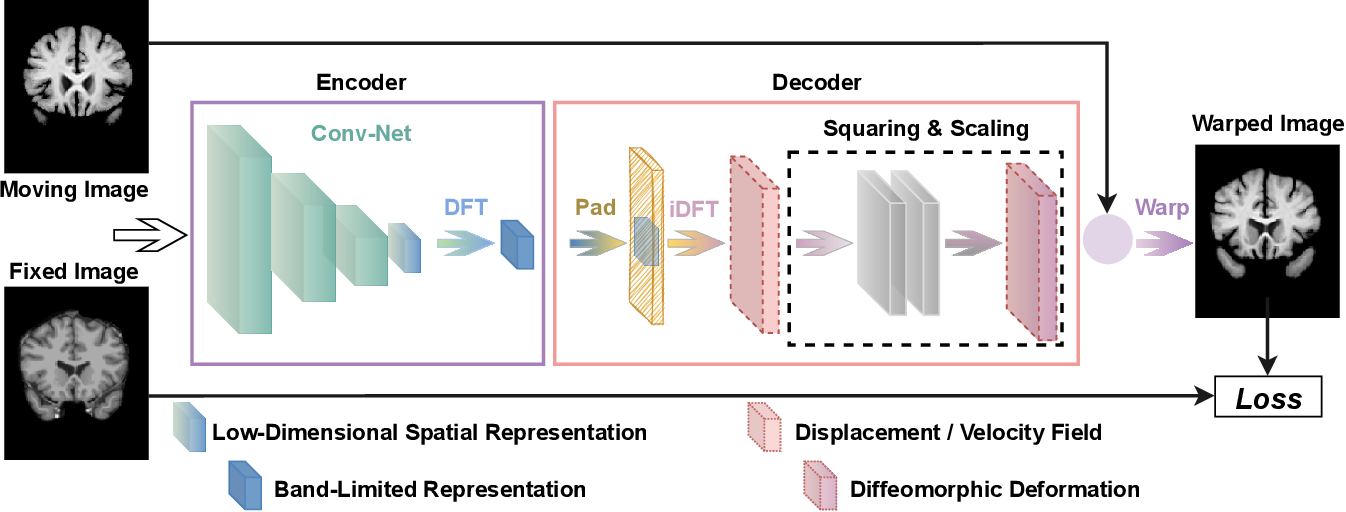
\includegraphics[width=\linewidth]{ArchitectureFourier-Net.png} 
	\caption{Architecture of \emph{Fourier-Net} taken from~\cite{Fourier-Net}. The encoder takes two images as an input and produces a band-limited displacement which is then padded and transformed to image space in the decoder. This output is the full-resolution displacement which is then used to warp the moving image for loss calculation based on its similarity to the fixed image.}
	\label{fig:Fourier-Net}
\end{figure}

\subsubsection{Encoder}	\label{SubSubSec:Encoder}
The encoder of \emph{Fourier-Net} consists of a CNN that generates the displacement field between the two inputs followed by a DFT layer that produces a band-limited representation of the full displacement field. The fully convolutional neural network (FCN) from \emph{SYMNet}~\cite{SYM-Net} was modified to function as the CNN of the encoder. Its (original) architecture (see Figure~\ref{fig:SYMNet}) is again based on the U-Net with a contracting and expanding path. The FCN concatenates the inputs images $X$ and $Y$ as a single 2-channel input and estimates two dense, non-linear displacement fields $\phi_{XY}$ and $\phi_{YX}$.  However only the displacement field for the moving image, denoted as $\mathbb{S}_\phi$, is needed since we are not interested in transforming the fixed image. This is actually a low dimensional representation because \emph{Fourier-Net} does not utilize the last two levels of the FCNs expanding path that would be needed to reconstruct the actual full-resolution displacement field $\phi$.

\begin{figure}[h] %tpb
	\centering
	\graphicspath{{images/}{\main/images/}}
	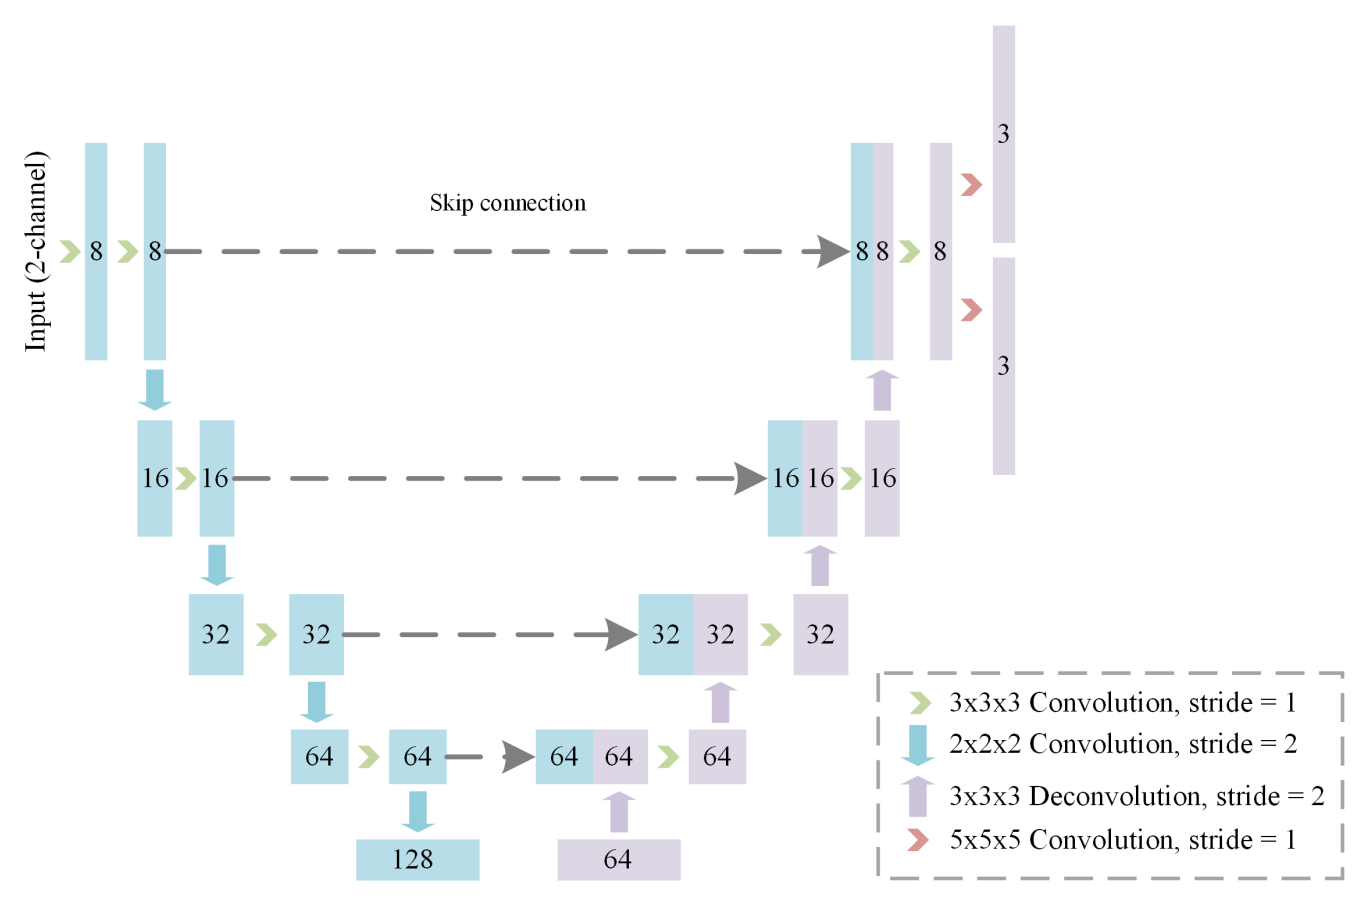
\includegraphics[width=\linewidth]{SYMNetArchitectureFCN.png} 
	\caption{Architecture of the FCN from \emph{SYMNet}~\cite{SYM-Net}. The contracting path of the encoder on the left is connected to the expanding path of the decoder on the right via skip connections. The blocks in blue and purple indicate the feature maps from the encoder and decoder respectively.}
	\label{fig:SYMNet}
\end{figure}


\noindent For each level in the contracting path of the FCN, two successive convolution layers are applied, which contain one $3 \times 3 \times 3$ convolution layer with a stride of 1, followed by a $3 \times 3 \times 3$ convolution layer with a stride of 2 to further compute the high-level features between the input images as well as downsampling the features by half until the lowest level of the network is reached. For each level in the expanding path of the FCN, the feature maps from the contracting path are concatenated through skip connections and apply $3 \times 3 \times 3$ convolution with a stride of 1 and $2 \times 2 \times 2$ de-convolution layer for upsampling the feature maps to twice of its size. At the end of the expanding path, two $5 \times 5 \times 5$ convolution layers with a stride of 1 are appended to the last convolution layer and generate the displacement fields $\theta_{XY}$ and $\theta_{YX}$~\cite{SYM-Net}. Each convolution layer in the FCN is followed by a rectified linear unit (ReLU) activation, except for the output convolution layer that does not have an activation function because \emph{Fourier-Net} only uses the first two levels of the expanding path, thus leading the FCN to generate a low dimensional representation $\mathbb{S}_\phi$ of the full-resolution displacement field $\phi$.\\
As discussed previously, the encoder aims to learn a displacement (or velocity) field in the band-limited Fourier domain. Intuitively, this may require convolutions to be able to handle complex-valued numbers, which can be done by using complex-valued CNNs~\cite{Trabelsi2017}, which are suitable when both input and output contain complex values, however these complex-valued operations sacrifice computational efficiency. Other approaches like \emph{DeepFlash}~\cite{DeepFlash} tackle this problem by converting the input images to the Fourier domain and using two individual real-valued CNNs to learn the real and imaginary parts separately. This, however, increases training and inference cost. To bridge the domain gap between real-valued spatial images and complex-valued band-limited displacement fields without increasing complexity, \emph{Fourier-Net} uses a DFT layer after the FCN. This is a simple and effective way to produce complex-valued band-limited displacement fields without the network needing to be able to handle complex values or learn a mapping between the image and frequency domain. The DFT applied to the displacement field $\phi$ can be defined as follows:
\begin{equation} \label{eq:DFT}
	[\mathcal{F}(\phi)]_{k,l} = \sum^{H-1}_{n=0} \sum^{W-1}_{m=0} \phi_{n,m} \cdot \exp \Bigg(i \cdot \bigg(\frac{2 \pi k}{H} \cdot n + \frac{2 \pi l}{W} \cdot m \bigg) \Bigg),
\end{equation}
where $\phi$ has size $H \times W$ with $H$ and $W$ being the spatial dimensions in 2D. $n \in [0,H-1]$ and $m \in [0,W-1]$ are the discrete indices in the spatial domain, and $k \in [0,H-1]$ and $l \in [0,W-1]$ are the discrete indices in the frequency domain with $i$ being the imaginary unit. However, $\phi$ in this equation is actually the low dimensional representation of the displacement field output by the modified FCN, which can be formulated as follows:
\begin{equation} \label{eq:FCN}
	\mathbb{S}_\phi = \text{FCN}(M,F;\Theta),
\end{equation}
with $M$ being the moving and $F$ the fixed image, as well as $\Theta$ representing the parameters of the FCN. Thus, the whole encoder can be defined as:
\begin{equation}\label{eq:encoder}
	\mathbb{B}_\phi = \mathcal{F}(\mathbb{S}_\phi) = \mathcal{F}(\text{FCN}(M,F;\Theta)),
\end{equation}
with the DFT layer $\mathcal{F}$, full-resolution spatial displacement field $\phi$ and the complex band-limited displacement field $\mathbb{B}_\phi$. The low dimensional representation $\mathbb{S}_\phi$ actually contains all the information of the band-limited Fourier coefficients in $\mathbb{B}_\phi$. As such, \emph{Fourier-Net} does not need to learn the coefficients of $\mathbb{B}_\phi$, but instead only the real-valued coefficients in $\mathbb{S}_\phi$, which is the low dimensional spatial representation of the full-resolution spatial displacement field $\phi$, which is then reconstructed by the decoder. 


\subsubsection{Decoder} \label{SubSubSec:Decoder}
The decoder contains no learnable parameters, as the expansive path is replaced with a zero-padding layer, an iDFT layer, and an optional squaring and scaling~\cite{ScaleAndSquare} layer. \\
The output from the encoder is the band-limited representation $\mathbb{B}_\phi$ in the frequency domain of the low dimensional displacement field $\mathbb{S}_\phi$ in the spatial domain. To recover the full-resolution displacement field $\phi$ in the spatial domain, we first pad the patch $\mathbb{B}_\phi$, containing mostly low frequency signals, to the original image resolution with zeros. We then feed the zero-padded complex-valued Fourier coefficients, denoted as $\mathcal{F}(\phi)$, to an iDFT layer consisting of two steps: shifting the Fourier coefficients from centers to corners and then applying the iDFT to convert them into the spatial domain:
\begin{equation} \label{eq:iDFT}
	\phi_{n,m} = \frac{1}{HW} \sum^{H-1}_{k=0} \sum^{W-1}_{l=0} \mathcal{D}_{k,l} [\mathcal{F}(\phi)]_{k,l} \cdot \exp \Bigg(i \cdot \bigg(\frac{2 \pi n}{H} \cdot k + \frac{2 \pi m}{W} \cdot l \bigg) \Bigg).
\end{equation}
The $H \times W$ sized sampling mask $\mathcal{D}$ is a low-pass filter that has zeros as entries if they are on the positions of high-frequency signals in $\phi$ and ones if they are on the low-frequency positions. Thus we can reconstruct the full spatial displacement field $\phi$ from $\mathbb{B}_\phi$ despite the latter being band-limited. Approaching the problem from the other side we can also think about working backwards from the final displacement. For this, after applying equation~(\ref{eq:DFT}), the low-frequency signals are shifted to a center patch of size $\frac{H}{a} \times \frac{W}{b}$ with $a = 2 \cdot Z_a$ and $ b = 2 \cdot Z_b$ where $ Z_a, Z_b \in \mathbb{Z}^+$, which is then center-cropped to get $\mathbb{B}_\phi$. This crop of $\mathcal{F}(\phi)$ can be reconstructed using the iDFT from equation~(\ref{eq:iDFT}) with the cropping functioning resembling a low-pass filter:
\begin{equation} \label{eq:decoder}
	[\mathbb{S}_\phi]_{n,m} = \frac{ab}{HW} \sum^{\frac{H}{a}-1}_{k=1} \sum^{\frac{W}{b}-1}_{l=1} [\mathbb{B}_\phi]_{k,l} \cdot \exp \Bigg(i \cdot \bigg(\frac{2 \pi a n}{H} \cdot k + \frac{2 \pi b m}{W} \cdot l \bigg) \Bigg),
\end{equation}
with $n \in [0, \frac{H}{a}-1]$ and $m \in [0, \frac{W}{b}-1]$ being the indices of the spatial domain, while $k \in [0, \frac{H}{a}-1]$ and $l \in [0, \frac{W}{b}-1]$ are the indices of the frequency domain with $i$ being the imaginary unit. Thus $\mathbb{S}_\phi$ actually contains all the necessary information from $\phi$, as long as they have the same low-frequency coefficients $\mathbb{B}_\phi$. This can be formulated as:
\begin{equation}
	[\mathbb{S}_\phi]_{n,m} = ab \cdot \phi_{an,bm},
\end{equation}
because most entries of $\mathcal{F}(\phi)$ are zeros, and the remaining values are exactly the same as in $\mathbb{B}_\phi$, which means that $\mathbb{S}_\phi$ contains all the information $\phi$ can provide. For this, however, $\mathbb{B}_\phi$ needs to be padded to the original image size first in order to get the full-resolution displacement and not a low dimensional representation. This ultimately shows that there is a unique mapping between $\mathbb{S}_\phi$ and $\phi$, which means that it is reasonable to use a network to learn $\mathbb{S}_\phi$ directly from image pairs and then reconstruct the displacement field in a very efficient manner~\cite{Fourier-Net}. The complete reconstruction process is visualized in Figure~\ref{fig:DecoderDisplacementField}.\\
As both padding and iDFT layers are differentiable, \emph{Fourier-Net} can be optimized via back-propagation. \emph{Fourier-Net} can use extra squaring and squaring layers~\cite{ScaleAndSquare,Dalca2018} in the decoder to turn the displacement field into a stationary velocity field. Typically seven scaling and squaring layers are used to impose such a diffeomorphism~\cite{Fourier-Net,Dalca2018}.

\begin{figure}[h] %tpb
	\centering
	\graphicspath{{images/}{\main/images/}}
	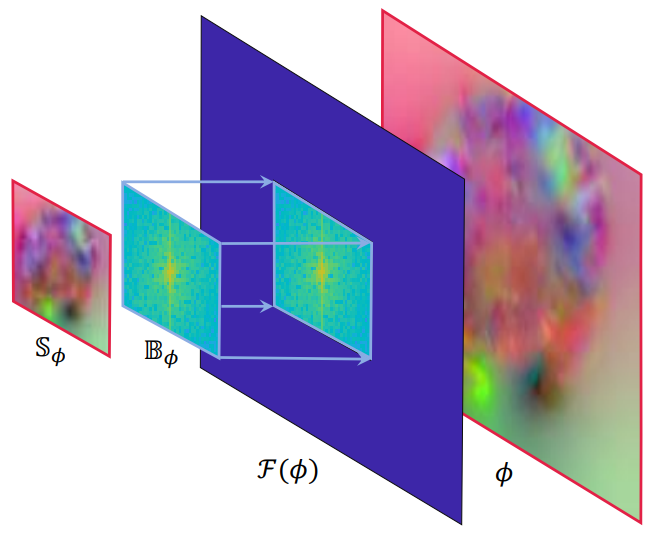
\includegraphics[width=.65\linewidth]{DecoderDisplacementField.png} 
	\caption{Reconstruction of the band-limited displacement field via the decoder taken from~\cite{Fourier-Net+}. The band-limited representation $\mathbb{B}_\phi$ is padded with zeros to the desired spatial resolution $\mathcal{F}(\phi)$ and then transformed to the full-resolution displacement $\phi$ using an iDFT.}
	\label{fig:DecoderDisplacementField}
\end{figure} 

\subsubsection{Diffeomorphic Transforms} \label{SubSubSec:DiffeomorphicTransforms}
Diffeomorphic deformations are differentiable and invertible, thus preserving topology, which is a desirable property for transformations. $\phi: \mathbb{R}^N \rightarrow \mathbb{R}^N$ represents the deformation that maps the coordinates from one image to coordinates in another image, as long as both images have the dimension $N$. When using a stationary velocity field representation like e.g. \emph{DARTEL}~\cite{DARTEL}, the deformation field is defined through the following ordinary differential equation (ODE)~\cite{Dalca2018}:
\begin{equation}
	\frac{\partial \phi^{(t)}}{\partial t} = v(\phi^{(t)}),
\end{equation}
where $\phi^{(0)} = \text{Id}$ is the identity transformation and $t$ is time. The final registration field $\phi^{(1)}$ can be obtained by integrating the stationary velocity field $v$ over $t = [0, 1]$. This is typically done by integration numerically using scaling and squaring~\cite{ScaleAndSquare}. The integration of a stationary ODE represents a one-parameter subgroup of diffeomorphisms. In group theory, $v$ is a member of the Lie algebra and is exponentiated to produce $\text{exp}(v) = \phi^{(1)}$, which is also a member of the Lie group. From the properties of one-parameter subgroups, for any scalars $t$ and $t'$, $\text{exp}((t + t') \cdot v) = \text{exp}(t \cdot v) \circ \text{exp}(t' \cdot v)$, where $\circ$ is a composition map associated with the Lie group. Starting from $\phi^{({1/2}^T)} = p + v(p)$ where $p$ is a map of spatial locations, we use the recurrence $\phi^{({1/2})^{t  1}} = \phi^{({1/2}^t)} \circ \phi^{({1/2}^t)}$ to obtain $\phi^1 = \phi^{(1/2)} \circ \phi^{(1/2)}$. $T$ is chosen so that $v \approx 0$~\cite{Dalca2018}. As diffeomorphic deformations are defined as smooth and invertible deformations, the output of the iDFT layer in \emph{Fourier-Net} can be regarded as a stationary velocity field $v$ instead of a displacement field $\phi$. In Figure~\ref{fig:Fourier-Net} scaling and squaring layers are visualized. These apply the diffeomorphic transformation in three steps~\cite{ScaleAndSquare}:
\begin{enumerate}
	\item Scaling: Divide the velocity field $v$ by a factor $2^N$ , so that $\frac{v}{2^N}$ is close to zero (depending on the desired accuracy).
	\item Exponentiation: Compute $\text{exp}\big(\frac{v}{2^N}\big) = \phi^{(1)}\big(\frac{v}{2^N}\big)$ with a first-order explicit numerical scheme.
	\item Squaring: $N$ recursive squarings of $\phi^{(1)}\big(\frac{1}{2^N}\big) = \text{exp}\big(\frac{v}{2^N}\big)$ to yield an accurate estimation of $\phi^{(1)}(1) = \phi^{(1)}\big(\frac{1}{2^N}\big)^{2^N} = \text{exp}\big(\frac{v}{2^N}\big)^{2^N} = \text{exp}(v)$.
\end{enumerate}
Thus, the diffeomorphic deformation can be efficiently calculated.


\subsubsection{Spatial Transformer} \label{SubSubSec:SpatialTransformer}
The warping layer of \emph{Fourier-Net} utilizes the \emph{Spatial Transformer}~\cite{SpatialTransformer}, which allows for spatial image manipulation within the network. This is a differentiable and learnable module for neural networks which applies a spatial transformation to a feature map during a single forward pass. The spatial transformer mechanism is split into three parts as seen in Figure~\ref{fig:SpatialTransformer}. First is the localization network, which takes the input and outputs the parameters for the transformation. These are then used to create a sample grid using the grid generator. Lastly, the sampler produces the output feature map based on the input at the grid points.\\
From the input feature map $U \in \mathbb{R}^{H \times W \times C}$ with width $W$, height $H$ and channels $C$ the localization network $f_{\text{loc}}$ computes the parameters $\theta = f_{\text{loc}}(U)$ of the transformation $\mathcal{T}_\theta$ which is later applied to the feature map. Thus the size of $\theta$ varies depending on the transformation. 
%(e.g. 6D for an affine transformation). 
The localization network function can both be implemented as a fully-connected network or as a CNN, but should include a final regression layer to produce the transformation parameters.\\
In order to warp the input feature map, each output pixel is computed by applying a sampling kernel centered at a particular location in the input feature map. The output pixels are defined to lie on a regular grid $G = {G_i}$ of pixels, forming an output feature map $V \in \mathbb{R}^{H' \times W' \times C}$, where $H'$ and $W'$ are the height and width of the grid with C again being the number of channels, which is the same for input and output. In order to perform a spatial transformation of the input feature map $U$, the sampler must take the set of sampling points $\mathcal{T}_\theta(G)$, along and produce the sampled output feature map $V$. Each coordinate $(x_i^s, y_i^s)$ in $\mathcal{T}_\theta(G)$ defines the spatial location in the input where a sampling kernel is applied to get the value at a particular pixel in the output:
\begin{equation}
	V_i^c = \sum^{H}_{n} \sum^{W}_{m} U_{nm}^c k(x_i^s - m; \Phi_x) k(y_i^s - n; \Phi_y),
\end{equation}
with $\Phi_x$ and $\Phi_y$ being the parameters for a generic sampling  kernel $k$ that defines the image interpolation, $U_{nm}^c$ is the value of the input feature maps at location $(n,m)$ in the channel $c \in [1, ..., C]$ and $V_i^c$ is the value for every pixel $i \in [1, ..., H'W']$ for the output feature map. Any sampling kernel can be used, as long as (sub-) gradients can be defined with respect to $(x_i^s, y_i^s)$ to allow the loss gradients to flow back not only to the input feature map, but also to the sampling grid coordinates and therefore back to the transformation parameters $\theta$ and localization network, thus enabling back-propagation~\cite{SpatialTransformer}.

\begin{figure}[h] %tpb
	\centering
	\graphicspath{{images/}{\main/images/}}
	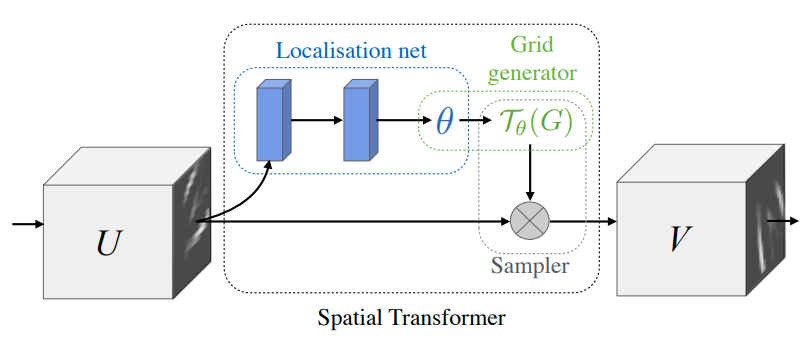
\includegraphics[width=\linewidth]{SpatialTransformer.png} 
	\caption{Architecture of the \emph{Spatial Transformer} taken from~\cite{SpatialTransformer}. The input feature map $U$ is passed to a localization network which outputs the transformation parameters $\theta$. The regular spatial grid $G$ over $V$ is transformed to the sampling grid $\mathcal{T}_\theta(G)$, which is applied to $U$ producing the warped output feature map $V$.}
	\label{fig:SpatialTransformer}
\end{figure}


\subsubsection{Loss Function} \label{SubSubSec:LossFunction}
The loss function consists of two parts to enable unsupervised learning, which are balanced using the scalar parameter $\lambda$. The first, $\mathcal{L}_{1}$, measures the similarity between the fixed image and the moving image after warping, while the second, $\mathcal{L}_{2}$, ensures a smooth displacement field. Thus, the unsupervised loss $\mathcal{L}$ can be calculated as follows:
\begin{equation}	\label{eq:unsupervisedLoss}
	\begin{split} 
		\mathcal{L}(\Theta) &= \min  \bigg( \mathcal{L}_{1} (\phi(\Theta))  + \lambda \cdot \mathcal{L}_{2} (\phi(\Theta)) \bigg) \\
		&= \min  \bigg( \mathcal{L}_{1} (v(\Theta))  + \lambda \cdot \mathcal{L}_{2} (v(\Theta)) \bigg),
	\end{split}
\end{equation}
for both displacement fields $\phi$ and velocity fields $v$. The first part of the loss function consists of:
\begin{equation} \label{eq:L1-LossDisp}
	\mathcal{L}_{1} (\phi(\Theta)) = \frac{1}{N} \sum^{N}_{i=1} \mathcal{L}_{Sim} (M_i \circ (\phi_i(\Theta) + \text{Id}) - F_i),
\end{equation}
where $\circ$ denotes the warping operation, $N$ the number of training pairs with moving images $M_i$ and fixed images $F_i$, $\Theta$ the network parameters, $\phi_i$ the displacement field and Id the identity grid. $\mathcal{L}_{Sim}$ determines the similarity between warped moving images and fixed images via MSE or NCC, and the second term of the unsupervised loss, $\mathcal{L}_{2}$, defines the smoothness regularization function that controls smoothness of the displacement fields:
\begin{equation} \label{eq:L2-LossDisp}
	\mathcal{L}_{2} (\phi(\Theta)) = \frac{1}{N} \sum^{N}_{i=1} || \nabla \phi_i(\Theta) ||^2_2,
\end{equation}
with $\nabla$ denoting the first order gradient and $|| \cdot ||_2^2$ denoting the squared $L_2$-Norm. \\
When using the squaring and scaling layers, thus making the deformation of the moving image diffeomorphic, the loss needs to be modified by replacing the displacement field $\theta$ with the velocity field $v$. Thus, both parts of the of the loss function need to be changed:
\begin{equation}	\label{eq:L1-LossVeloc}
	\mathcal{L}_{1} (v(\Theta)) = \frac{1}{N} \sum^{N}_{i=1} \mathcal{L}_{Sim} (M_i \circ Exp(v_i(\Theta) - F_i),
\end{equation}
\begin{equation} \label{eq:L2-LossVeloc}
	\mathcal{L}_{2} (v(\Theta)) = \frac{1}{N} \sum^{N}_{i=1} || \nabla v_i(\Theta) ||^2_2  \bigg .
\end{equation}


\subsection{Fourier Net+} \label{SubSec:Fourier-Net+}
\emph{Fourier-Net+}, as the name suggests, is an extension of Fourier-Net which takes the band-limited spatial representation of the images as input, instead of their original full-resolution counterparts. This leads to further reduction in the number of convolutional layers in the contracting path of the network, resulting in a decrease of parameters, memory usage, and computational operations. This makes \emph{Fourier-Net+} even more efficient than its predecessor~\cite{Fourier-Net+}.

\begin{figure}[h] %tpb
	\centering
	\graphicspath{{images/}{\main/images/}}
	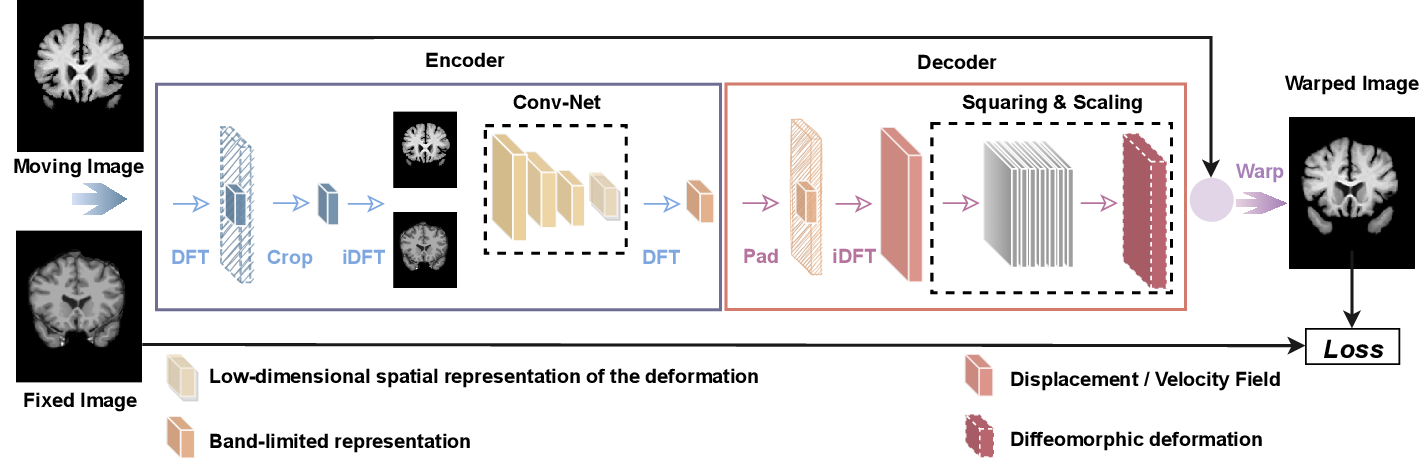
\includegraphics[width=\linewidth]{ArchitectureFourier-Net+.png} 
	\caption{Architecture of \emph{Fourier-Net+} taken from~\cite{Fourier-Net+}. The encoder has a additional compression step to reduce the input size of the images compared to \emph{Fourier-Net}. This is achieved by center-cropping the k-space of the images obtained via a DFT and then reconstructing them via an iDFT to get a compressed version of the inputs without the higher frequencies present. The rest of the network is the same as for \emph{Fourier-Net}.}
	\label{fig:Fourier-Net+}
\end{figure}

\noindent As seen in Figure~\ref{fig:Fourier-Net+}, the network architecture is almost the same as for \emph{Fourier-Net} (see Figure~\ref{fig:Fourier-Net} for comparison). However, while the decoder, and thus the loss function, remain the same, the encoder is slightly altered to make the network even more efficient. For this, similarly to the decoder, a DFT is used, however this time the idea is applied to the input images. These are first transformed into the Fourier domain, then low-pass filtered by center-cropping and finally reconstructed from their band-limited representation back into the spatial domain via an iDFT. The two images, now compressed, are the input for the encoder of \emph{Fourier-Net}, meaning the CNN and following DFT. However, due to the band-limiting before the CNN, the latter can be made much more light-weight, thus reducing computational cost. This is visualized in Figure~\ref{fig:Fourier-Net+CNN}. Thus, \emph{Fourier-Net+} too is overall lighter than the baseline \emph{Fourier-Net} in terms of the number of parameters and computations. However, such a light network may face limitations in accurately capturing complex deformations. To counter this potential weakness, the authors propose a cascaded version of \emph{Fourier-Net+}, which uses multiple versions of \emph{Fourier-Net+} cascaded one after the other to achieve a better overall displacement field~\cite{Fourier-Net+}. A schematic for this can be seen in Figure~\ref{fig:Fourier-Net+Cascaded}.

\begin{figure}[h] %tpb
	\centering
	\graphicspath{{images/}{\main/images/}}
	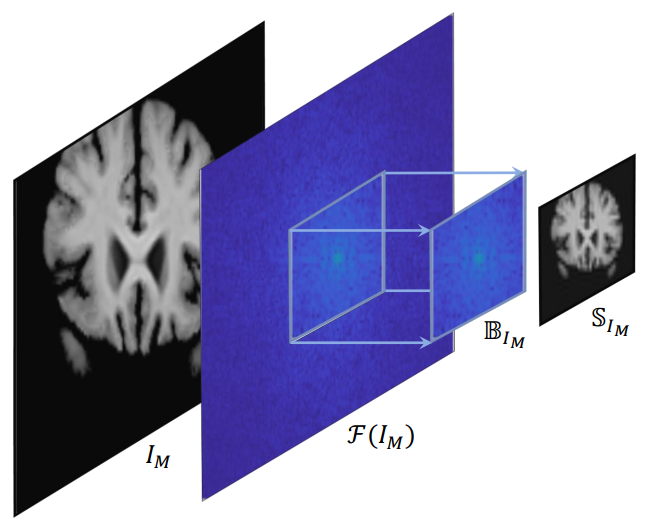
\includegraphics[width=.65\linewidth]{CompressionEncoder.png} 
	\caption{Compression in the frequency domain of the encoder used in \emph{Fourier-Net+} taken from~\cite{Fourier-Net+}. The frequencies $\mathcal{F}(I_M)$ are obtained via a DFT and then center-cropped to obtain a band-limited version $\mathbb{B}_{I_M}$. The compressed image $\mathbb{S}_{I_M}$ is then reconstructed via a iDFT.}
	\label{fig:Fourier-Net+EncoderCompression}
\end{figure}


\subsubsection{Changes to the Encoder} \label{SubSubSec:ChangesEncoder}
In order to further reduce the amount of computational operations, \emph{Fourier-Net+} discards the early layers of the encoder. Instead, a DFT $\mathcal{F}(I_M)$ followed by a center-crop to produce the band-limited representation $\mathbb{B}_{I_M}$ in the frequency domain and iDFT are used to get the spatial patch $\mathbb{S}_{I_M}$, while the rest of the encoder from \emph{Fourier-Net} stays the same. The input $I_M$ is thus compressed to a lower resolution (i.e. band-limited) using the frequency space, which reduces the computational cost. This process is visualized in Figure~\ref{fig:Fourier-Net+EncoderCompression}. The encoder of \emph{Fourier-Net+} has several convolutional layers less in the contracting path compared to \emph{Fourier-Net}, which leads to a further accelerated registration process while reducing the memory footprint. These advantages are visualized in Figure~\ref{fig:Fourier-Net+CNN} where the amount of different layers between a conventional U-Net, \emph{Fourier-Net} (with the smaller decoder) and \emph{Fourier-Net+} (with a smaller encoder and decoder) are shown.

\begin{figure}[h] %tpb
	\centering
	\graphicspath{{images/}{\main/images/}}
	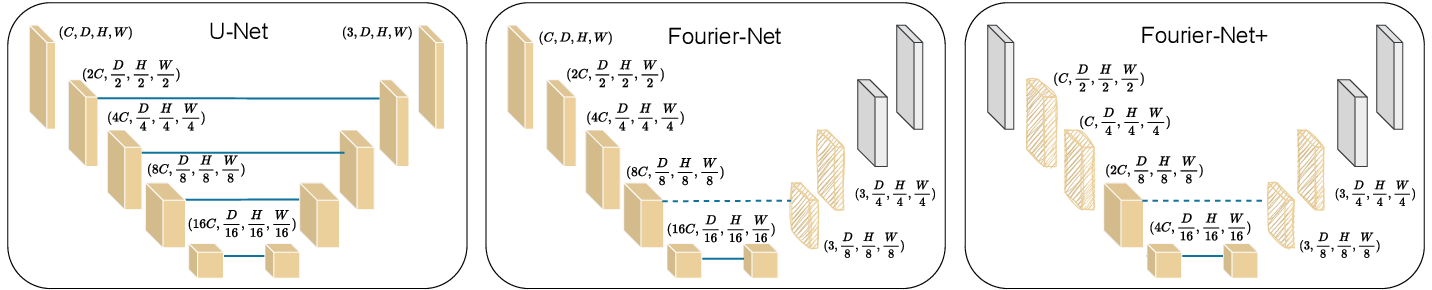
\includegraphics[width=\linewidth]{ArchitectureFourier-Net+CNN.png} 
	\caption{Architecture of the CNN for a typical U-Net, \emph{Fourier-Net} and \emph{Fourier-Net+} taken from~\cite{Fourier-Net+}. The latter have far less trainable network parameters due to only computing a band-limited displacement. \emph{Fourier-Net+} additionally has a smaller encoder due to compressing the input images.} % making it even more efficient
	\label{fig:Fourier-Net+CNN}
\end{figure}

\subsubsection{Effects of Cascading} \label{SubSubSec:EffectsCascading}
As seen in the previous section, \emph{Fourier-Net+} is lighter than \emph{Fourier-Net} due to the band-limited representation of both images and deformations lowering the number of parameters and computations. This, however, can lead to limitations when trying to accurately capture complex deformations. To this end, a cascaded version of \emph{Fourier-Net+} called \emph{K$\times$Fourier-Net+} (see Figure~\ref{fig:Fourier-Net+Cascaded}), with $K$ denoting the amount of cascades, can be used where the warped image of one cascade is used as the moving image of the next. It is important to note that the weights are not shared between cascades. The squaring and scaling layers are applied after the last cascade, in case a diffeomorphic deformation is wanted. The same is true for the calculation of the loss function.\\
In order to more accurately describe this version of \emph{Fourier-Net+} one can look at the in- and outputs of the different cascades. The first cascade of \emph{K$\times$Fourier-Net+} has the moving image $I_M$ and fixed image $I_F$ as inputs. While the latter always stays the same for all cascades the warped image $I_M^{w(1)}$ from the first cascade is used as input for the second cascade instead of the original moving image. Thus, in general $I_M^{w(k-1)}$ and $I_F$ are the inputs for a cascade $k \in [1, K]$ with output $\delta \phi^{(k)}$. Furthermore, $I_M^{w(k)}$ can be defined as:
\begin{equation}
	I_M^{w(k)} = ((((I_M \circ \delta \phi^{(1)}) \circ \delta \phi^{(2)}) \circ \dots ) \circ \delta \phi^{(k-1)}) \circ \delta \phi^{(k)} = I_M \circ  \phi^{(k)},
\end{equation}
with $\phi^{(k)}$ being the displacement field computed by composing the outputs of the first cascade up to the $k$-th cascade:
\begin{equation}
	\phi^{(k)} = \delta \phi^{(1)} \circ \delta \phi^{(2)} \circ \dots \circ \delta \phi^{(k-1)} \circ \delta \phi^{(k)}.
\end{equation}
Thus, the output displacement field of the $K$-th cascade $\phi^{(K)}$ is the final displacement used to warp $I_M$, the original moving image, in order to compute the loss~\cite{Fourier-Net+}.

\begin{figure}[h] %tpb
	\centering
	\graphicspath{{images/}{\main/images/}}
	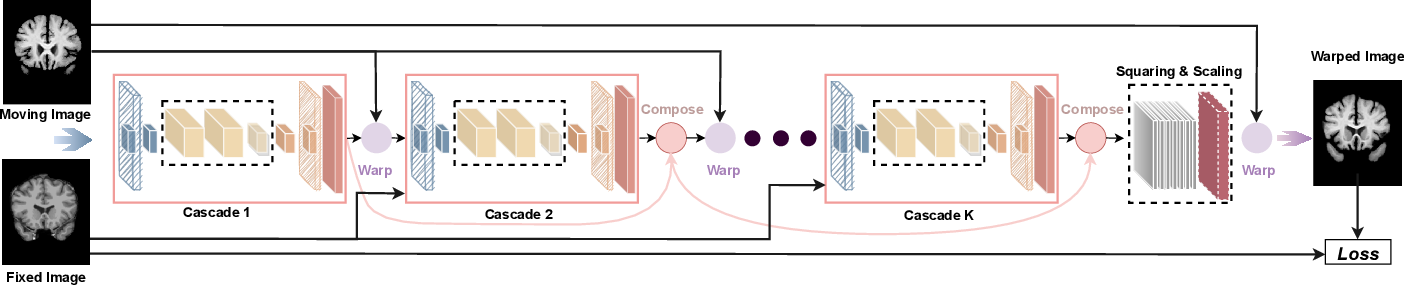
\includegraphics[width=\linewidth]{ArchitectureFourier-Net+Cascaded.png} 
	\caption{Cascaded version of \emph{Fourier-Net+} taken from~\cite{Fourier-Net+}. Multiple instances of \emph{Fourier-Net+} can be cascaded with independent weights for better performance as the network itself is very memory efficient.}
	\label{fig:Fourier-Net+Cascaded}
\end{figure}


\section{Datasets}	\label{Sec:Datasets}
In the following chapter, the datasets used in this thesis are presented. The \emph{Automated Cardiac Diagnosis Challenge (ACDC)} dataset~\cite{ACDC} from the \emph{MICCAI 2017} conference was mainly used for ablation studies and parameter tests. While it contains no k-space data, segmentations are given for the end-systolic and end-diastolic frames of the test set, which can be used to evaluate the registration performance using the Dice score. \\
The \emph{CMRxRecon} dataset~\cite{CMRxRecon} from the \emph{CMRxRecon2023} challenge specializes in CMR imaging. It was used for downstream-tests regarding MR image reconstruction. The cardiac MRI k-space data was used for the evaluation motion-compensated reconstruction pipeline. It contains subsampled data, but does not provide segmentations for multi-coil data.

\subsection{ACDC Dataset} \label{SubSec:ACDC}
The \emph{ACDC} dataset contains cardiac cine MRI short-axis data from 150 subjects that were divided into 5 subgroups (4 pathological, 1 healthy). For each subject systolic (see Figure~\ref{fig:Image_ACDC_systolic}) and diastolic frames (see Figure~\ref{fig:Image_ACDC_diastolic}) are provided with corresponding segmentations (see Figure~\ref{fig:Segmentation_ACDC_systolic} and ~\ref{fig:Segmentation_ACDC_diastolic}), which enables direct comparison via e.g. the Dice score. The segmentations contain only four values with 0, 1, 2 and 3 representing pixels located in the background, in the right ventricle (RV) cavity, in the myocardium, and in the left ventricle (LV) cavity. The frames themselves are 3D volumes with size $216 \times 256 \times 10$, thus ten image slices can be extracted which each have size $216 \times 256$. The same holds true for the segmentation, which means that both the image data and segmentations can generated in the same manner.\\
For the training data, the original 4D data was used as we do not require the segmentations for the end-systolic and end-diastolic frames. As the 4D data has size $216 \times 256 \times 10 \times 30$ we can extract 30 frames for each of the ten slices. These can be sorted into 251376 image pairs for training. For the validation and test data the end-systolic and end-diastolic frames with their segmentations were used giving us 641 image pairs each.\\
As the dataset only contained images reconstructed from fully sampled data, the data had to manually be subsampled. This was done by first obtaining the k-space data via a FFT and then subsampling the k-space for $=4$, $R=8$ and $R=10$ before going back to image space using a iFFT. This naive reconstruction lead to the typical artifacts (see Figure~\ref{fig:ManuelSubsampling_ACDC}) that the networks will be tested against.

\begin{figure}[h]%tpb
	\centering
	\begin{subfigure}{0.49\textwidth}
    		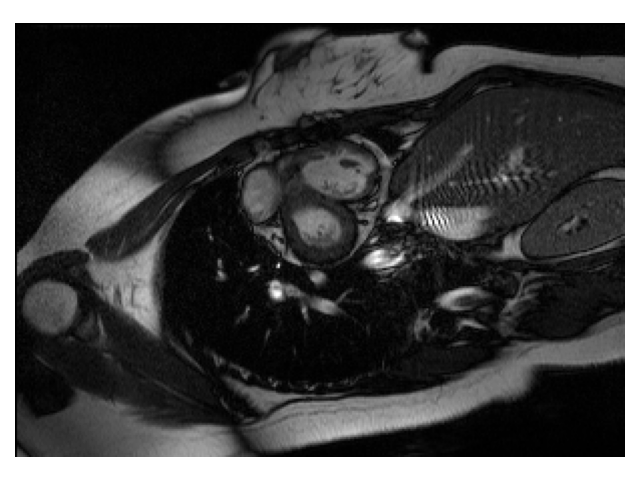
\includegraphics[width=\textwidth]{./Images/Image_ACDC_systolic.png}
    		\caption{Image of systolic phase.}
    		\label{fig:Image_ACDC_systolic}
	\end{subfigure}
	\hfill
	\begin{subfigure}{0.49\textwidth}
    		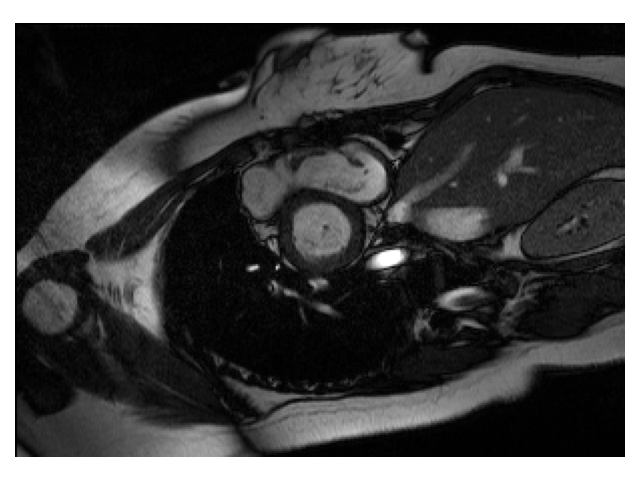
\includegraphics[width=\textwidth]{./Images/Image_ACDC_diastolic.png}
    		\caption{Image of diastolic phase.}
    		\label{fig:Image_ACDC_diastolic}
	\end{subfigure} 
	\\
	\begin{subfigure}{0.49\textwidth}
    		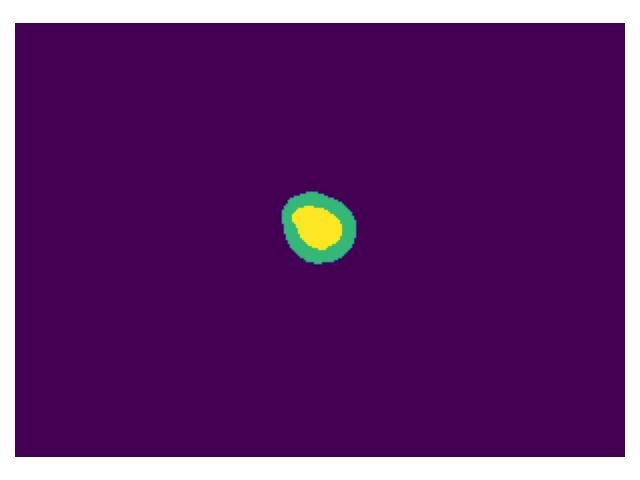
\includegraphics[width=\textwidth]{./Images/Segmentation_ACDC_systolic.png}
    		\caption{Segmentation of systolic phase.}
    		\label{fig:Segmentation_ACDC_systolic}
	\end{subfigure}
	\hfill
	\begin{subfigure}{0.49\textwidth}
    		
\includegraphics[width=\textwidth]{./Images/Segmentation_ACDC_diastolic.png}
    		\caption{Segmentation of diastolic phase.}
    		\label{fig:Segmentation_ACDC_diastolic}
	\end{subfigure}
	\caption{Example images for systolic (a) and diastolic frames (b) with corresponding segmentations (c), (d) taken from the \emph{ACDC} dataset~\cite{ACDC}.}
	\label{fig:}
\end{figure}

\begin{figure}[h] %tpb
	\centering
	\begin{subfigure}{0.32\textwidth}
    		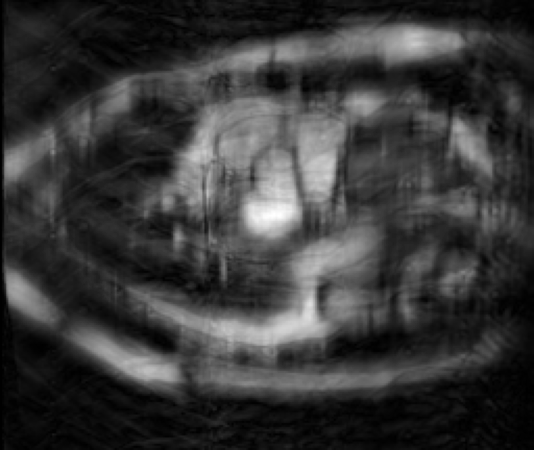
\includegraphics[width=\textwidth]{./Images/ManualSubsamplingACDC_Mode1.png}
    		\caption{Manuel subsampling for $R=4$.}
    		\label{fig:ManualSubsamplingACDC_Mode1}
	\end{subfigure}
	\hfill 
	\begin{subfigure}{0.32\textwidth}
    		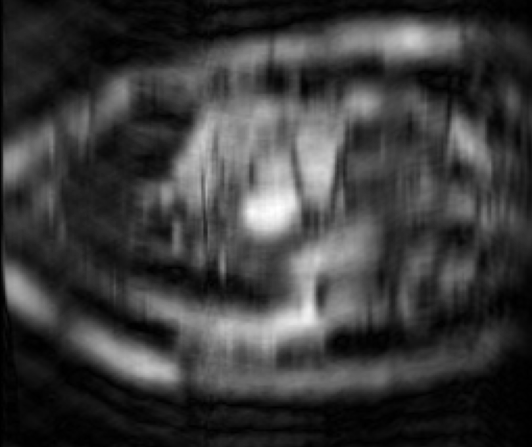
\includegraphics[width=\textwidth]{./Images/ManualSubsamplingACDC_Mode2.png}
    		\caption{Manuel subsampling for $R=8$.}
    		\label{fig:ManualSubsamplingACDC_Mode2}
	\end{subfigure}
	\hfill 
	\begin{subfigure}{0.32\textwidth}
    		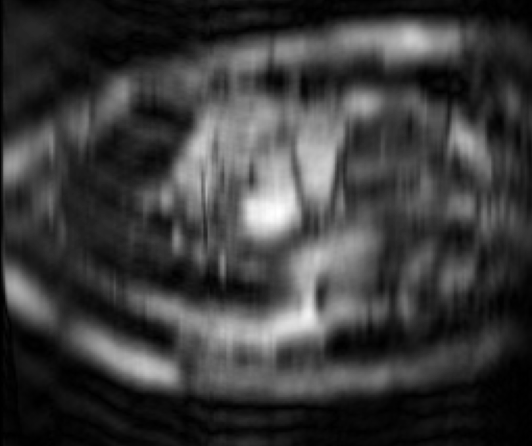
\includegraphics[width=\textwidth]{./Images/ManualSubsamplingACDC_Mode3.png}
    		\caption{Manuel subsampling for $R=10$.}
    		\label{fig:ManualSubsamplingACDC_Mode3}
	\end{subfigure}
	\caption{Example images for the manual subsampling $R=4$, $R=8$, and $R=10$ of the \emph{ACDC} data.}
	\label{fig:ManuelSubsampling_ACDC}
\end{figure}


\subsection{CMRxRecon Dataset} \label{SubSec:CMRxRecon}
The \emph{CMRxRecon} dataset includes fully sampled and subsampled multi-coil k-space data, as well as auto-calibration lines from the center region. This includes imaging of different anatomical views like long-axis (2-chamber, 3-chamber, and 4-chamber) and short-axis (SAX). There is a total of 120 training data, 60 validation data, and 120 test data from healthy volunteers. In contrast to the \emph{ACDC} dataset, \emph{CMRxRecon} contains only the raw k-space data. One of the goals of the challenge is the reconstruction from subsampled k-space data, e.g. accelerated MRI scans.\\
As the data was recorded in the k-space (see Figure~\ref{fig:k-space}) and stored as \emph{.mat} files it first needs to reconstructed to images in order to use them for training and testing of neural networks. First, an iFFT needs to be performed to get from k-space to image space, however the multi-coil data needs further processing. The effect of different coil sensitivities in their respective images can be seen in Figure~\ref{fig:Coils}, where each coil focuses on a specific area of the image. These images are then stitched together during reconstruction to produce a coil-combined image with great overall contrast. Often the simple RSS method is used where the resulting image is simply the root of the sum of the squared coil images~\cite{Roemer1990}. \\
The dataset, as mentioned before, contains fully sampled as well as subsampled k-space data (see Figure~\ref{fig:fullySampled} and Figure~\ref{fig:subSampled}), with the latter being used to accelerate the MRI acquisition process. This is done by subsampling the k-space data with mask. The center region of the k-space is usually fully sampled, but the outer regions are subsampled~\cite{SamplingStrategies}. The dataset contains subsampled k-space data for 4x, 8x and 10x acceleration with the latter of course leading to more artifact in the reconstructed image due to the subsampling. This can be seen in Figure~\ref{fig:subSampledImage}, where the image reconstructed from 4x accelerated ($R=4$) k-space data seems blurred when compared to the fully sampled ($R=0$) one in Figure~\ref{fig:fullySampledImage}. \\
For all experiments, the SAX view data was used. As image sizes between patients can vary slightly, interpolation was used to standardize the images to a size of $246 \times 512$ to avoid further problems with e.g. loss calculation. Additionally, min-max-normalization is used to standardize the data range for all images to $[0,1]$. The reconstructed images were stored for every image slice for every patient. Thus, all frames for an image slice were in a single folder to enable easy access for later data load-in.


\begin{figure}[H]%tpb
	\centering
	\graphicspath{{images/}{\main/images/}}
	\begin{subfigure}{0.45\textwidth}
    		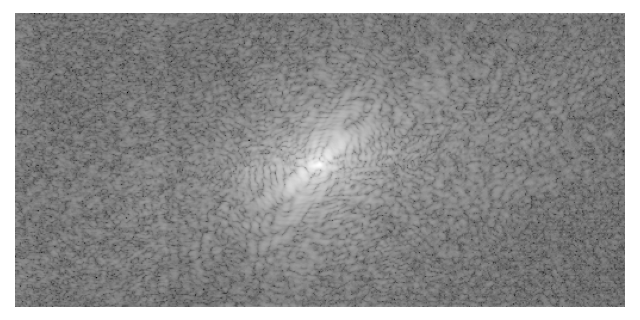
\includegraphics[width=\textwidth]{k-space_fullysampled.png}
    		\caption{A fully sampled k-space with low frequencies in the center and higher frequencies in the outer regions.}
    		\label{fig:fullySampled}
	\end{subfigure}
	\hfill
	\begin{subfigure}{0.45\textwidth}
    		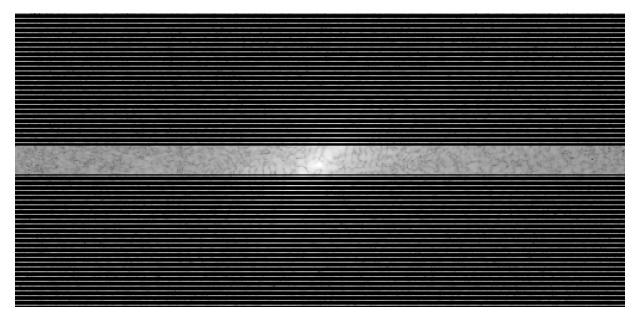
\includegraphics[width=\textwidth]{k-space_subsampled.png}
    		\caption{A 4x accelerated k-space. The center region remains fully sampled while higher frequencies are omitted.}
    		\label{fig:subSampled}
	\end{subfigure}\\
	\begin{subfigure}{0.45\textwidth}
    		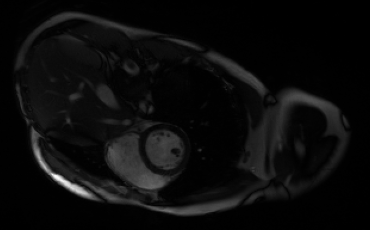
\includegraphics[width=\textwidth]{image_fullysampled.png}
    		\caption{Corresponding high quality image reconstructed from the fully sampled k-space.}
    		\label{fig:fullySampledImage}
	\end{subfigure}
	\hfill
	\begin{subfigure}{0.45\textwidth}
    		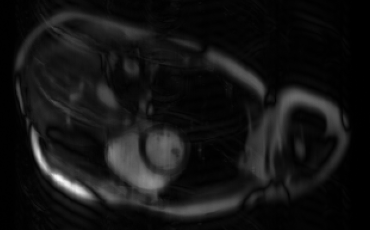
\includegraphics[width=\textwidth]{image_subsampled.png}
    		\caption{Corresponding image reconstructed from the subsampled k-space with blurring and aliasing artifacts.}
    		\label{fig:subSampledImage}
	\end{subfigure}
	\caption{Fully sampled and subsampled k-space data from the from the \emph{CMRxRecon} dataset~\cite{CMRxRecon} with corresponding images (empty background was cropped out).}
	\label{fig:k-space}
\end{figure}

\begin{figure}[H]%tpb
	\centering
	\graphicspath{{images/}{\main/images/}}
	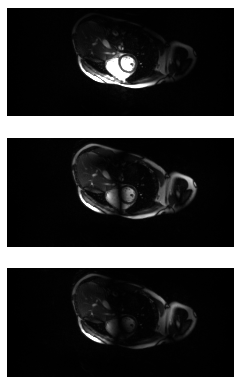
\includegraphics[width=\textwidth]{Coils.png} 
	\caption{MRI images for three different coils from the \emph{CMRxRecon} dataset~\cite{CMRxRecon}. The different sensitive areas can clearly be seen as they have significantly higher pixel values compared to the rest of the image. The background was cropped out from the images as the effect is not visible there. Note that the sensitivities are slightly corrupted as the coils were compressed to 10 coils for all the scans.}
	\label{fig:Coils}
\end{figure}

\subsection{Simulated Motion} \label{SubSec:SimulatedMotion}
In order to test the motion-compensated reconstruction pipeline, strongly motion-corrupted data is needed. As none of the datasets described previously meet these demands, the motion needed to be simulated manually. To simulate this motion or mis-triggering, two different strategies were used. First, line swapping in the k-space, and second, non-linear lung transformations.

\subsubsection{K-space Line Swapping}
First, a strategy similar to~\cite{Oksuz2020} was used, swapping $z$ k-space lines between the frames in k-space. The frames used for this all stem from the same slice and the information is swapped for all coils. The new fully sampled frames were then subsampled to the needed acceleration using the subsampling masks. Then, an iFT and RSS was used to generate the corrupted images. An example for $z=\{16,32\}$ can be seen in Figure~\ref{fig:LineSwapping}. 


% Line Swapping next to each other
\begin{figure}[h] %tpb
	\centering
	\begin{subfigure}{0.325\textwidth}
    		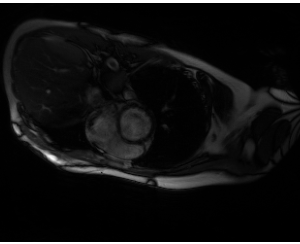
\includegraphics[width=\textwidth]{./Images/LineSwappingOriginal.png}
    		\caption{Original image.}
    		\label{fig:LineSwappingOriginal}
	\end{subfigure}
	\hfill
	\begin{subfigure}{0.325\textwidth}
    		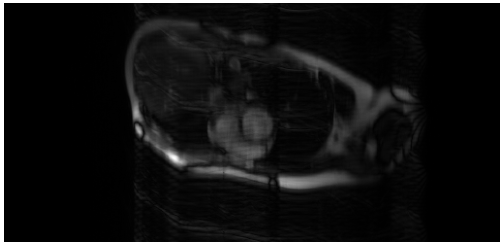
\includegraphics[width=\textwidth]{./Images/LineSwapping16.png}
    		\caption{Line swapping $z=16$.}
    		\label{fig:LineSwapping16}
	\end{subfigure}
	\hfill
	\begin{subfigure}{0.325\textwidth}
    		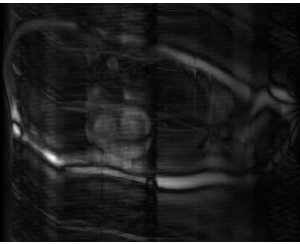
\includegraphics[width=\textwidth]{./Images/LineSwapping32.png}
    		\caption{Line swapping $z=32$.}
    		\label{fig:LineSwapping32}
	\end{subfigure}
	\caption{Examples for line swapping for $z=\{16,32\}$ with $R=4$ subsampling compared to the original fully sampled image.}
	\label{fig:LineSwapping}
\end{figure}

%% Line Swapping under each other
%\begin{figure}[h] %tpb
%	\centering
%	\begin{subfigure}{0.8\textwidth}
%    		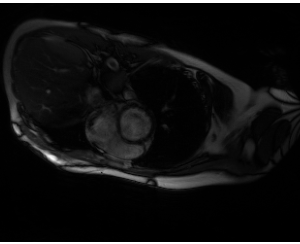
\includegraphics[width=\textwidth]{./Images/LineSwappingOriginal.png}
%    		\caption{Original image.}
%    		\label{fig:LineSwappingOriginal}
%	\end{subfigure}
%	\\
%	\begin{subfigure}{0.8\textwidth}
%    		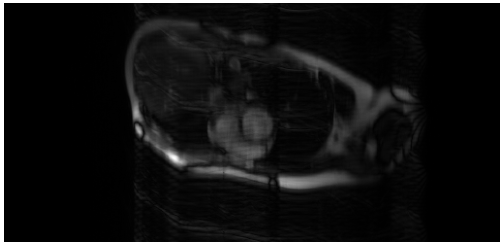
\includegraphics[width=\textwidth]{./Images/LineSwapping16.png}
%    		\caption{Line swapping $z=16$.}
%    		\label{fig:LineSwapping16}
%	\end{subfigure}
%	\\
%	\begin{subfigure}{0.8\textwidth}
%    		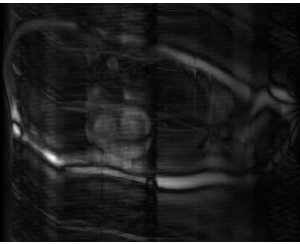
\includegraphics[width=\textwidth]{./Images/LineSwapping32.png}
%    		\caption{Line swapping $z=32$.}
%    		\label{fig:LineSwapping32}
%	\end{subfigure}
%	\caption{Examples for line swapping with $R=4$ subsampling compared to the original fully sampled image.}
%	\label{fig:LineSwapping}
%\end{figure}

\subsubsection{Non-Linear Lung Transformations}
Second, a simulation of non-linear lung movement was performed by randomly deforming the images and then generating the motion-corrupted k-space data from them. For this, a random displacement generator from~\cite{LAPNet} was used to generate random displacements in image space with a maximum velocity of 0.1. These displacements were then applied to each coil image before using an FT to convert from image to k-space, thereby modeling lung motion by expanding a cardiac time point into different respiratory time points for the multi-coil k-space data. This was done for $L=4$ additional lung motion frames for each cardiac frame. An example of such additional frames with artificial lung movement can be as seen in Figure~\ref{fig:LungMotion}.

% lung motion 2x2
\begin{figure}[h] %tpb 
	\centering
	\begin{subfigure}{0.475\textwidth}
    		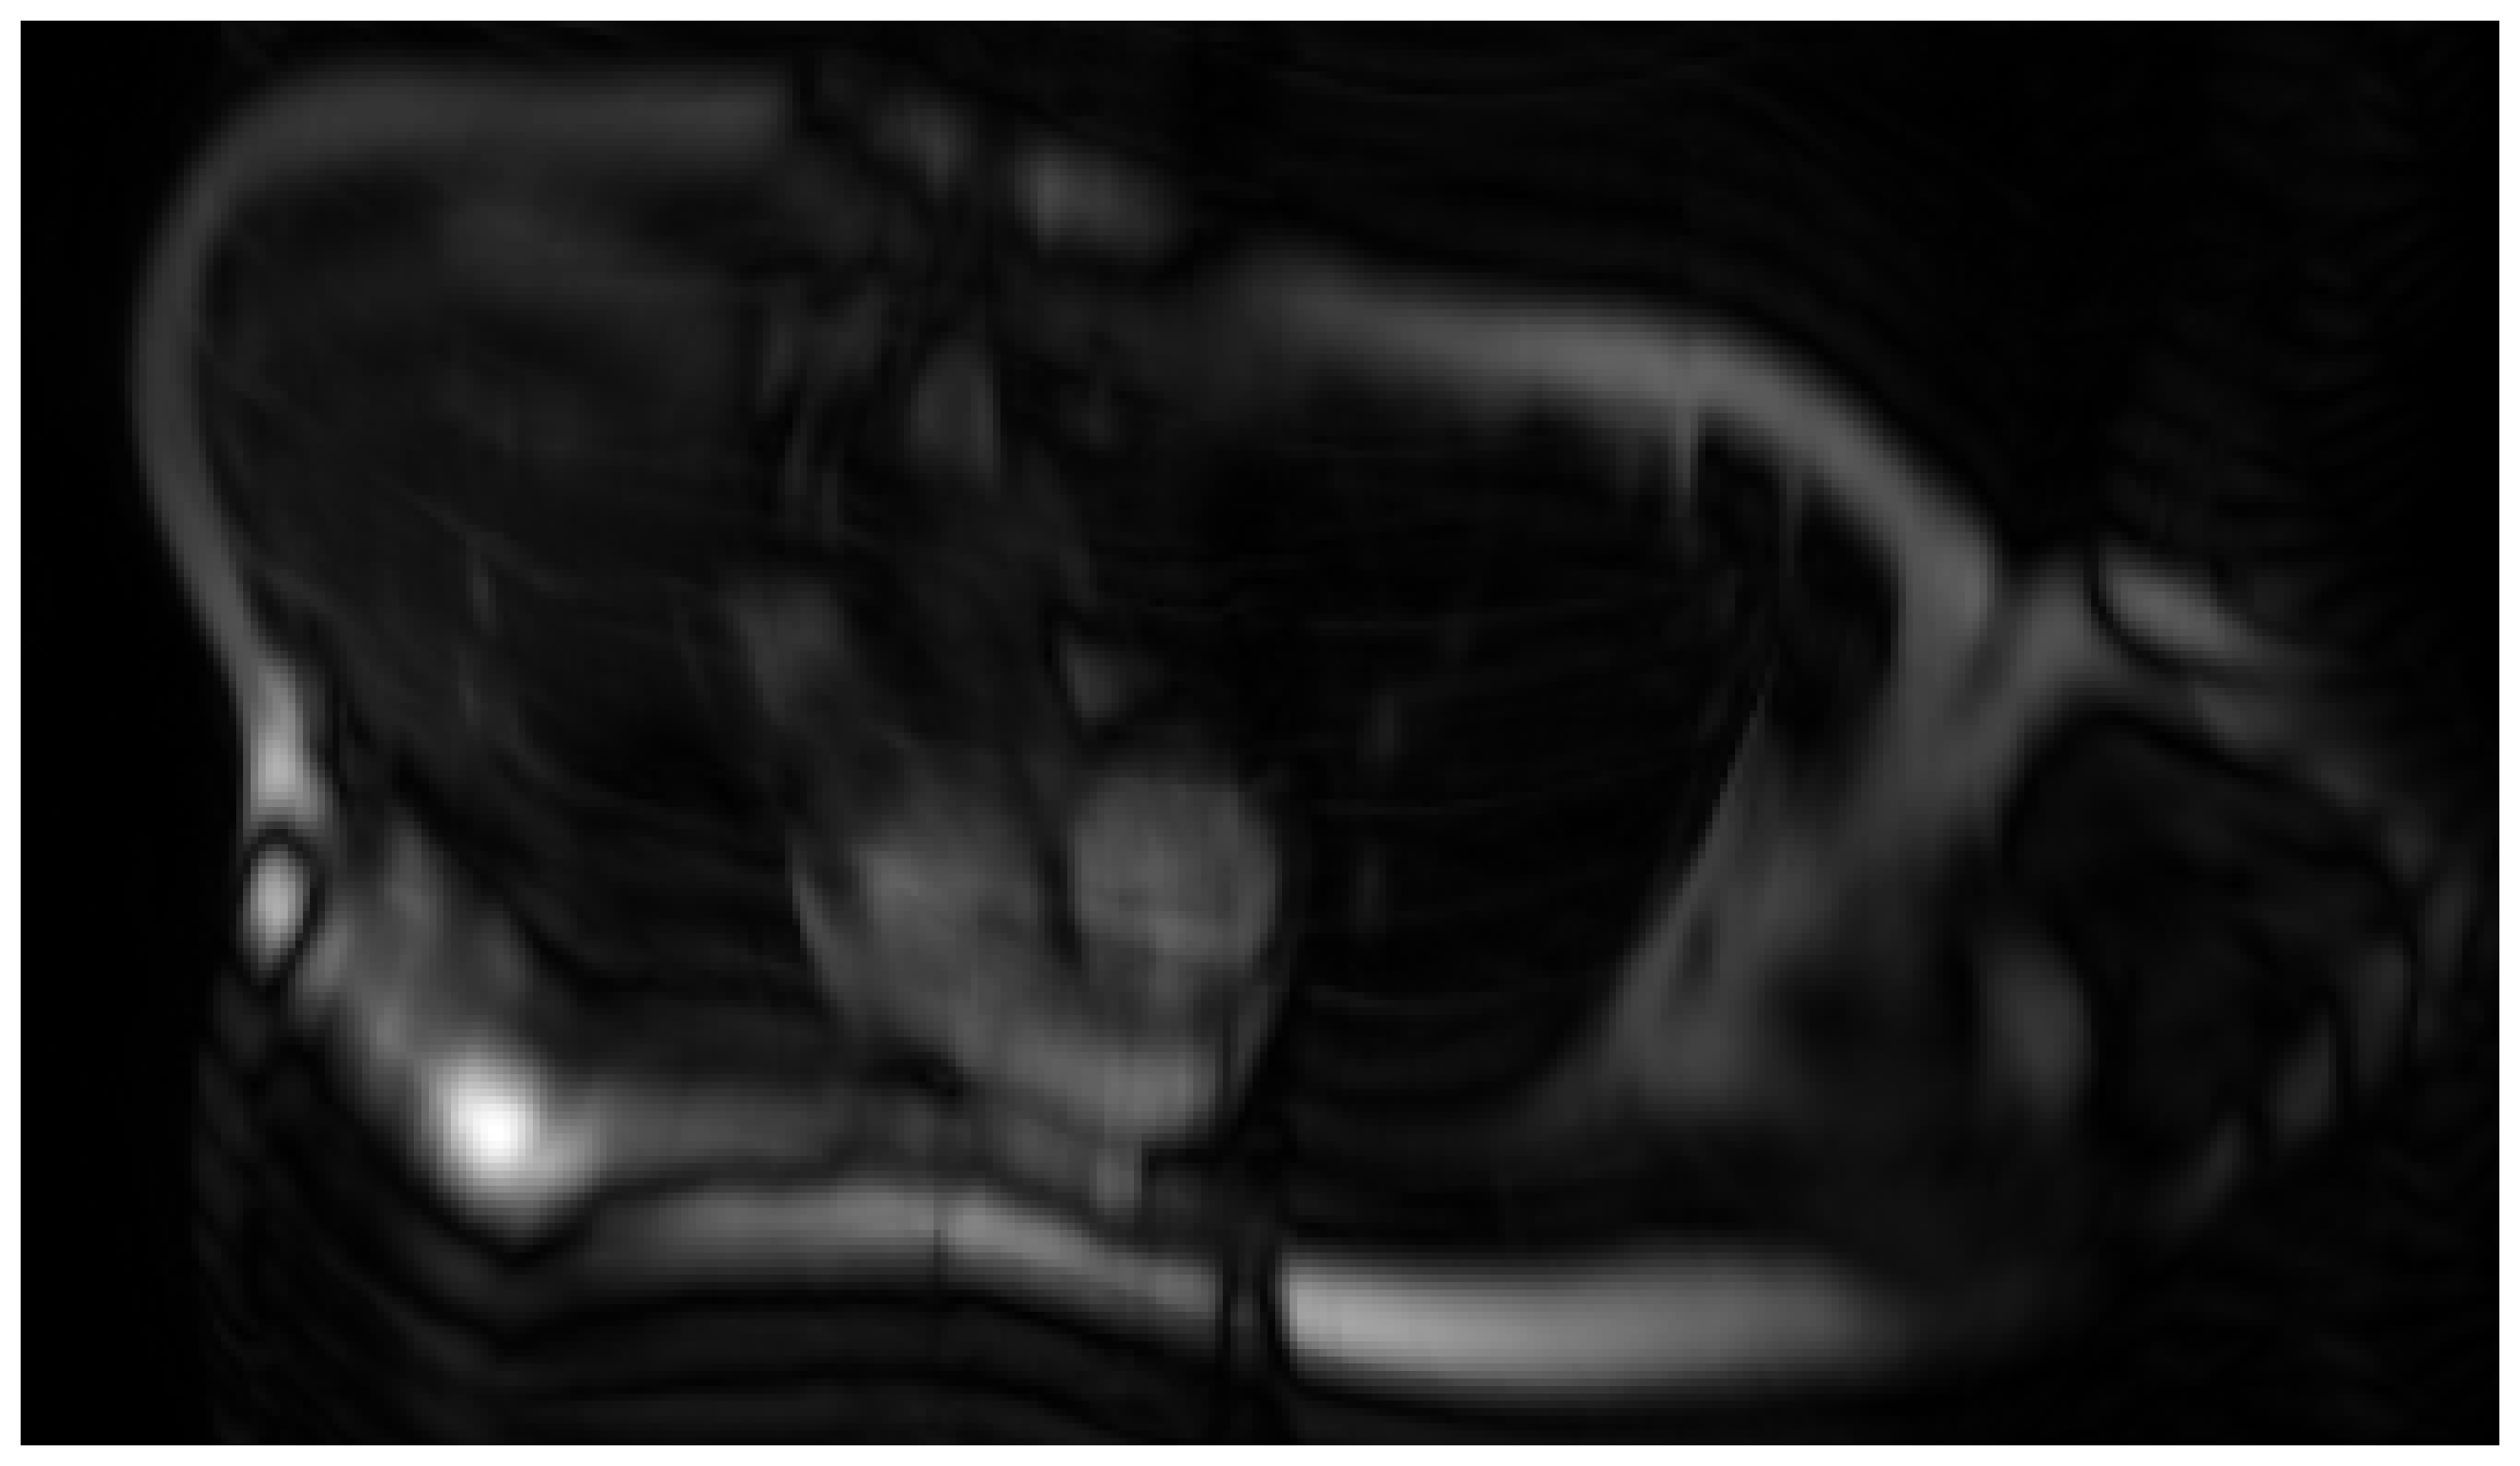
\includegraphics[width=\textwidth]{./Images/LungMotion1.png}
    		%\caption{First subfigure.}
    		\label{fig:LungMotion1}
	\end{subfigure}
	\hfill
	\begin{subfigure}{0.475\textwidth}
    		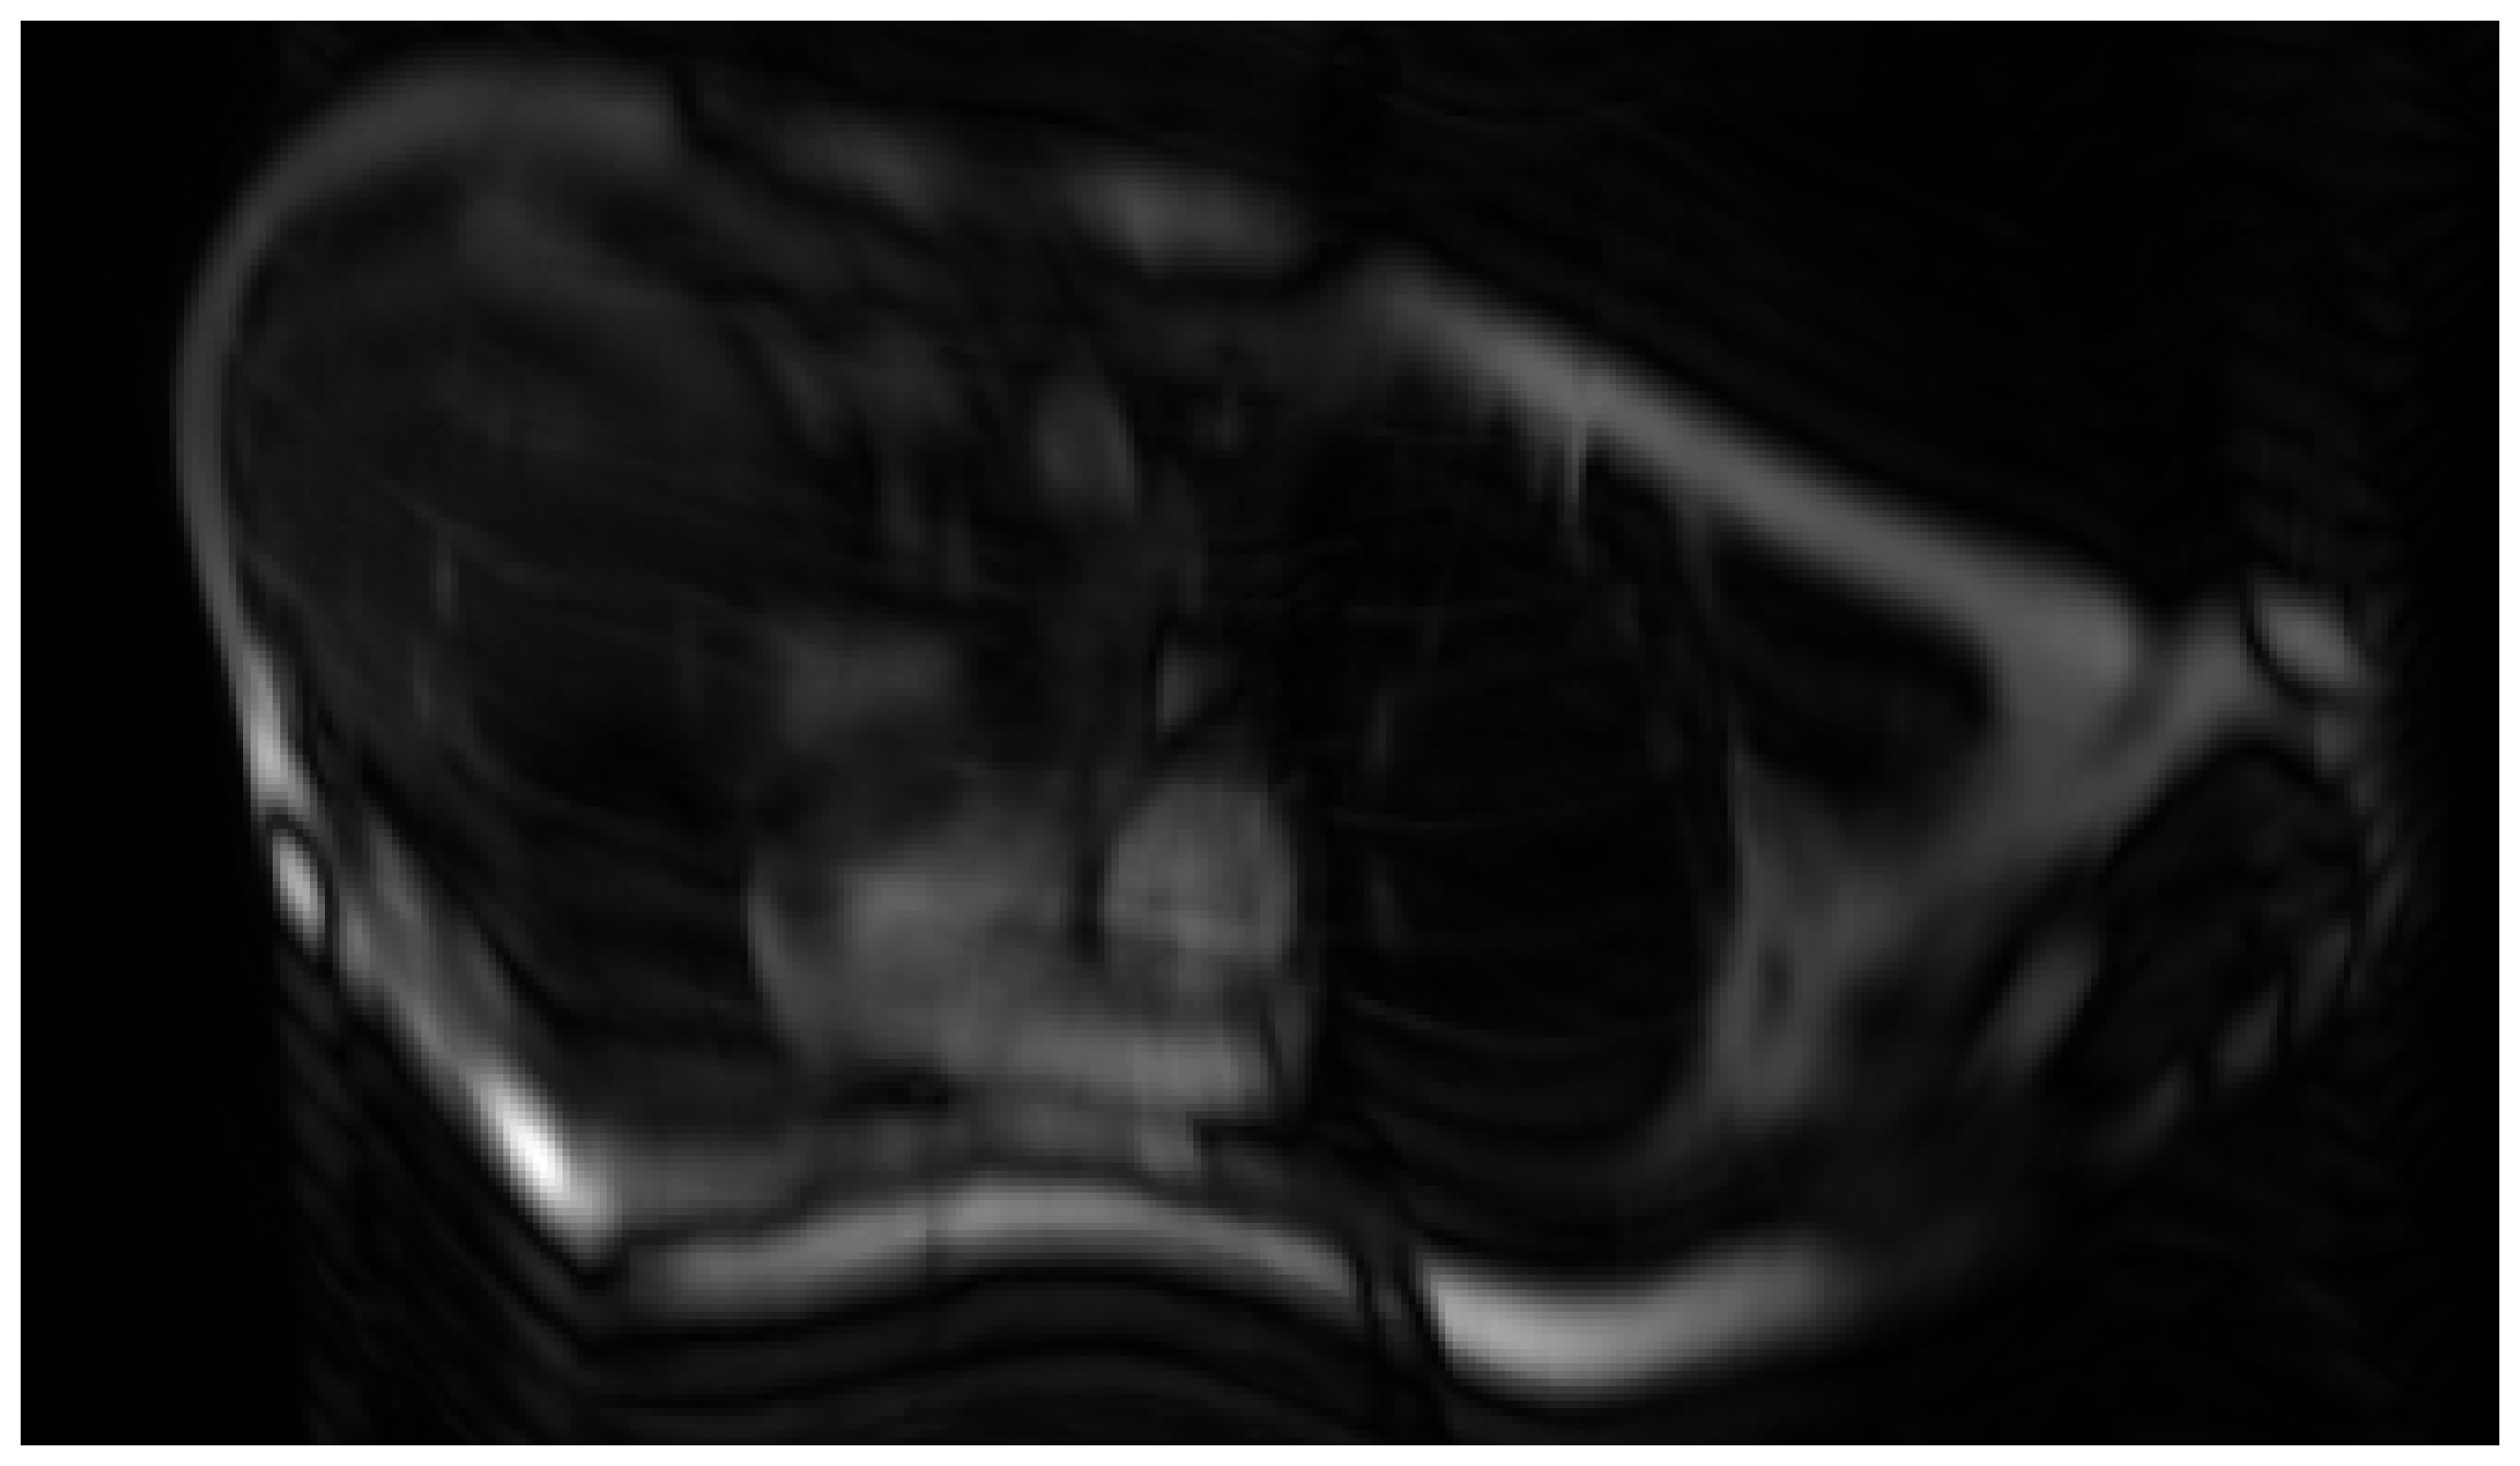
\includegraphics[width=\textwidth]{./Images/LungMotion2.png}
    		%\caption{Second subfigure.}
    		\label{fig:LungMotion2}
	\end{subfigure}
	\\
	\begin{subfigure}{0.475\textwidth}
    		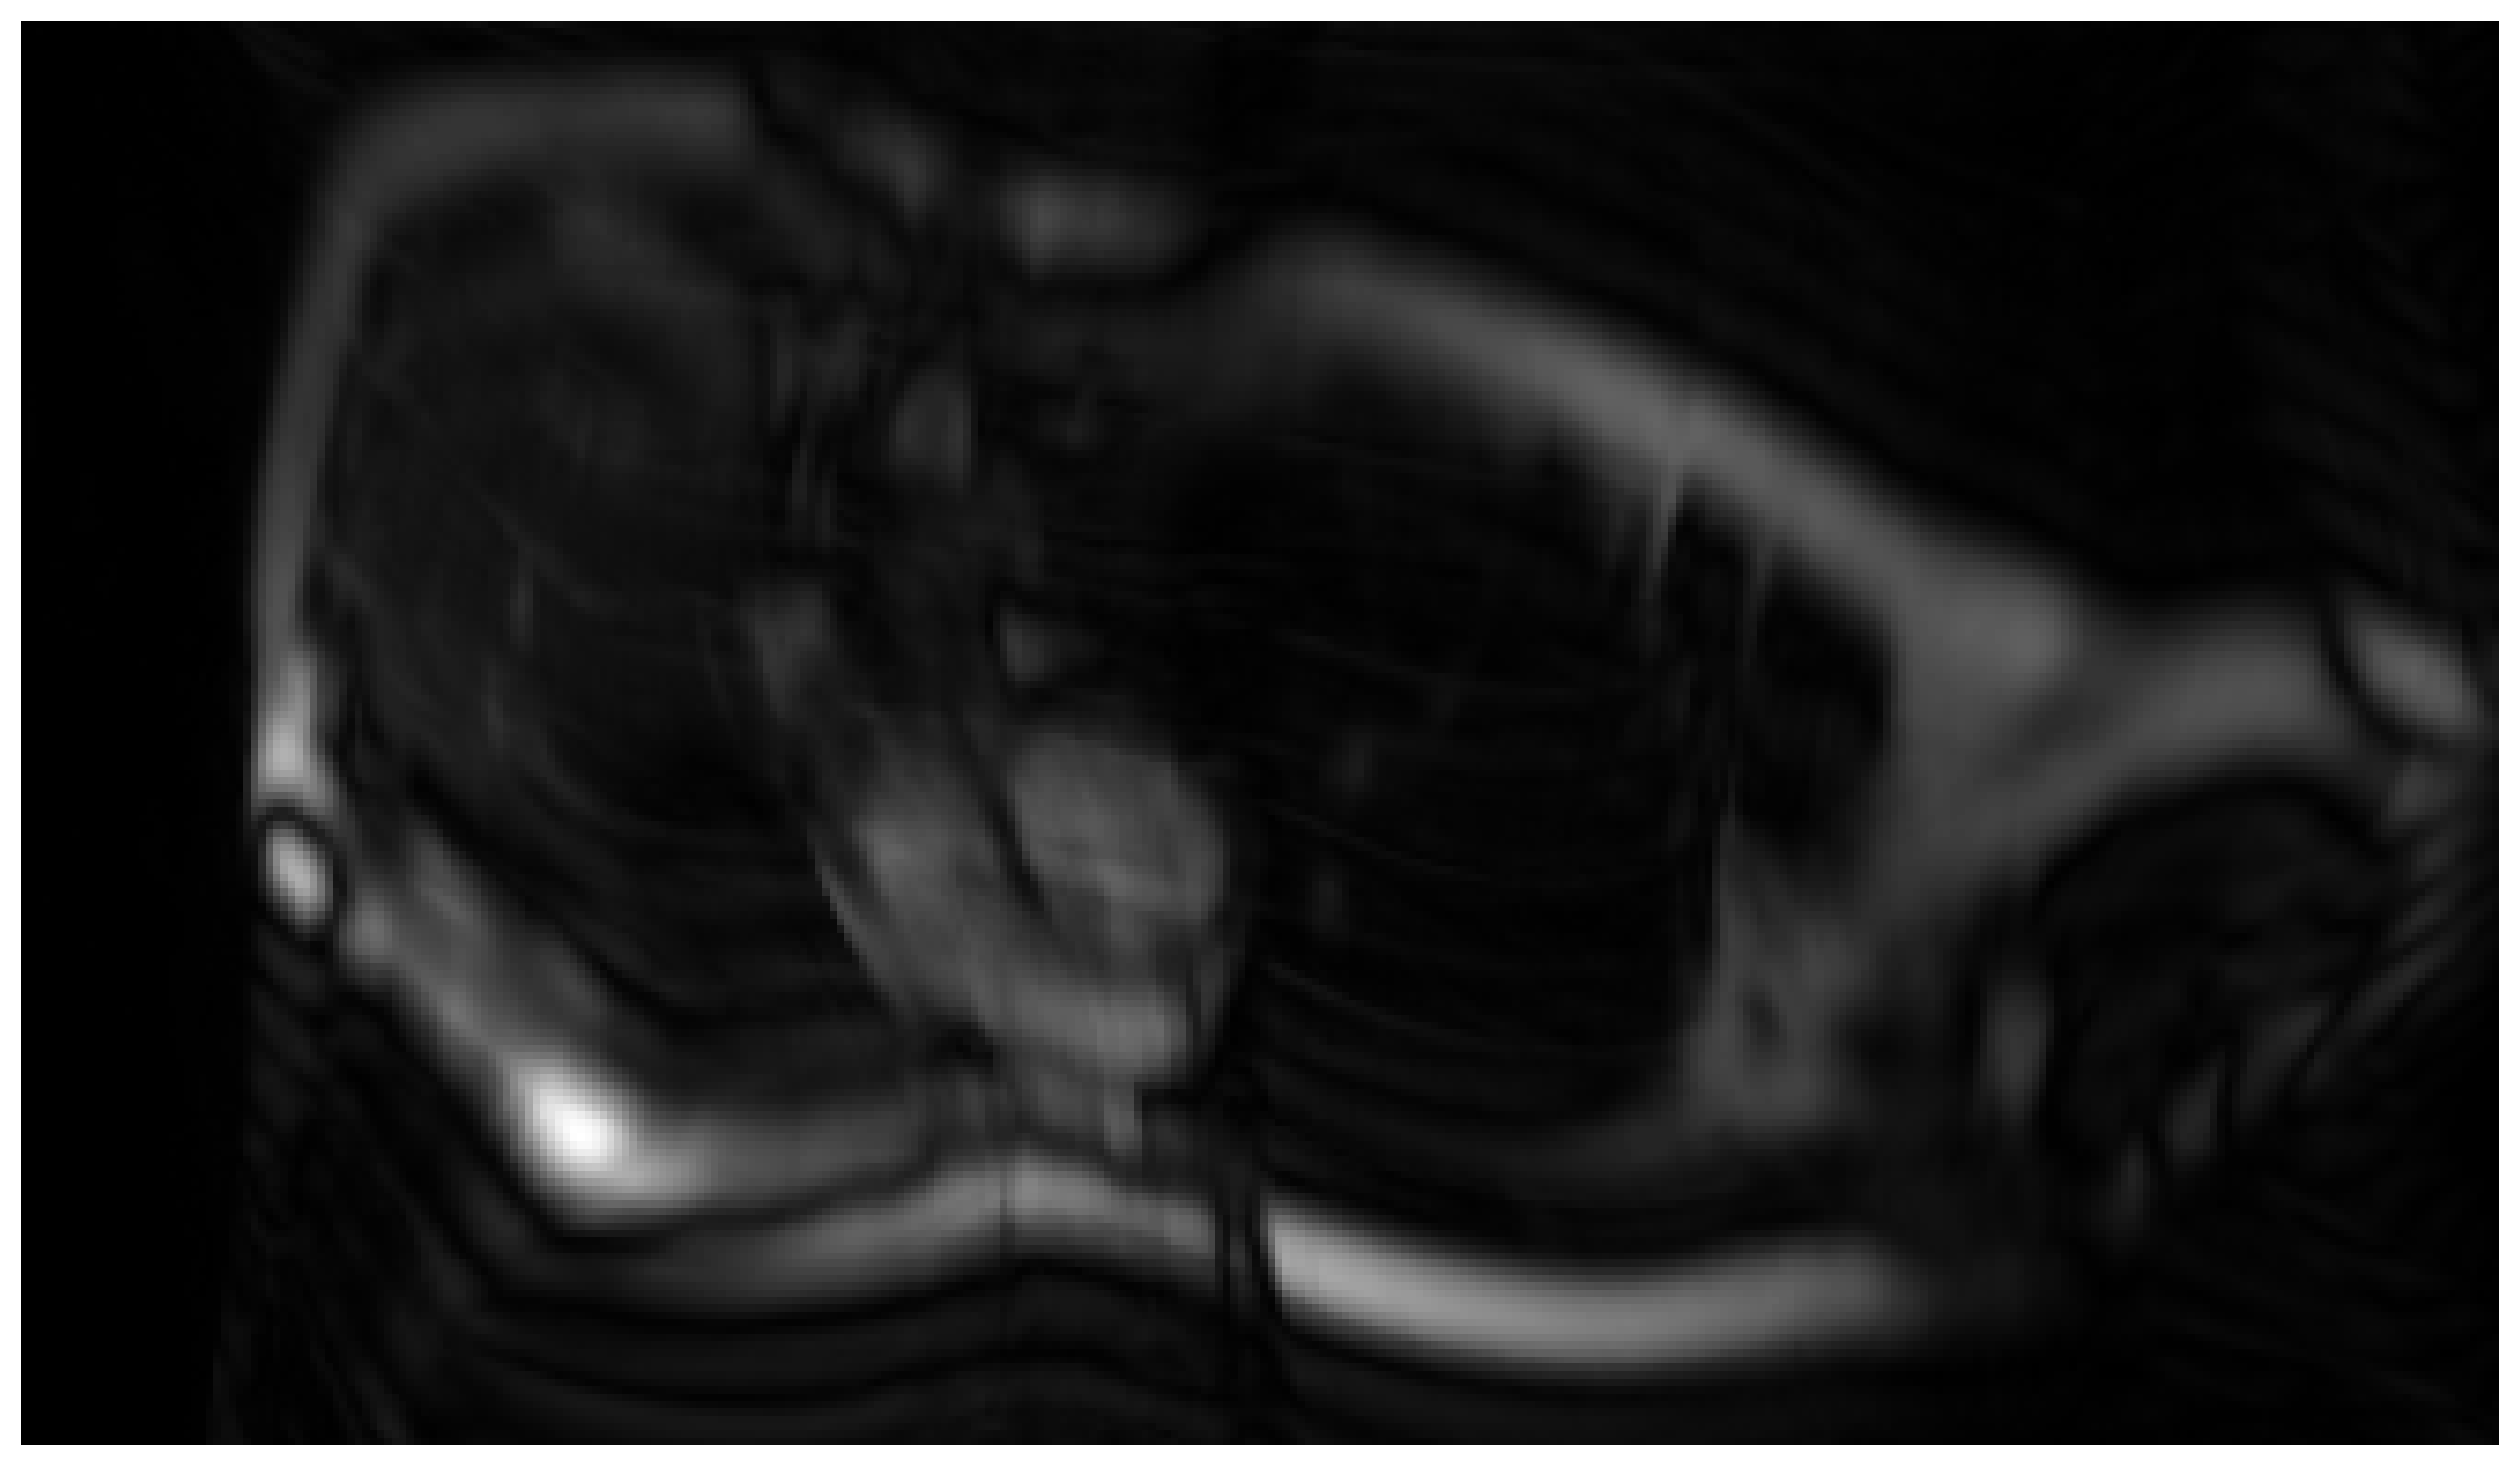
\includegraphics[width=\textwidth]{./Images/LungMotion3.png}
    		%\caption{First subfigure.}
    		\label{fig:LungMotion3}
	\end{subfigure}
	\hfill
	\begin{subfigure}{0.475\textwidth}
    		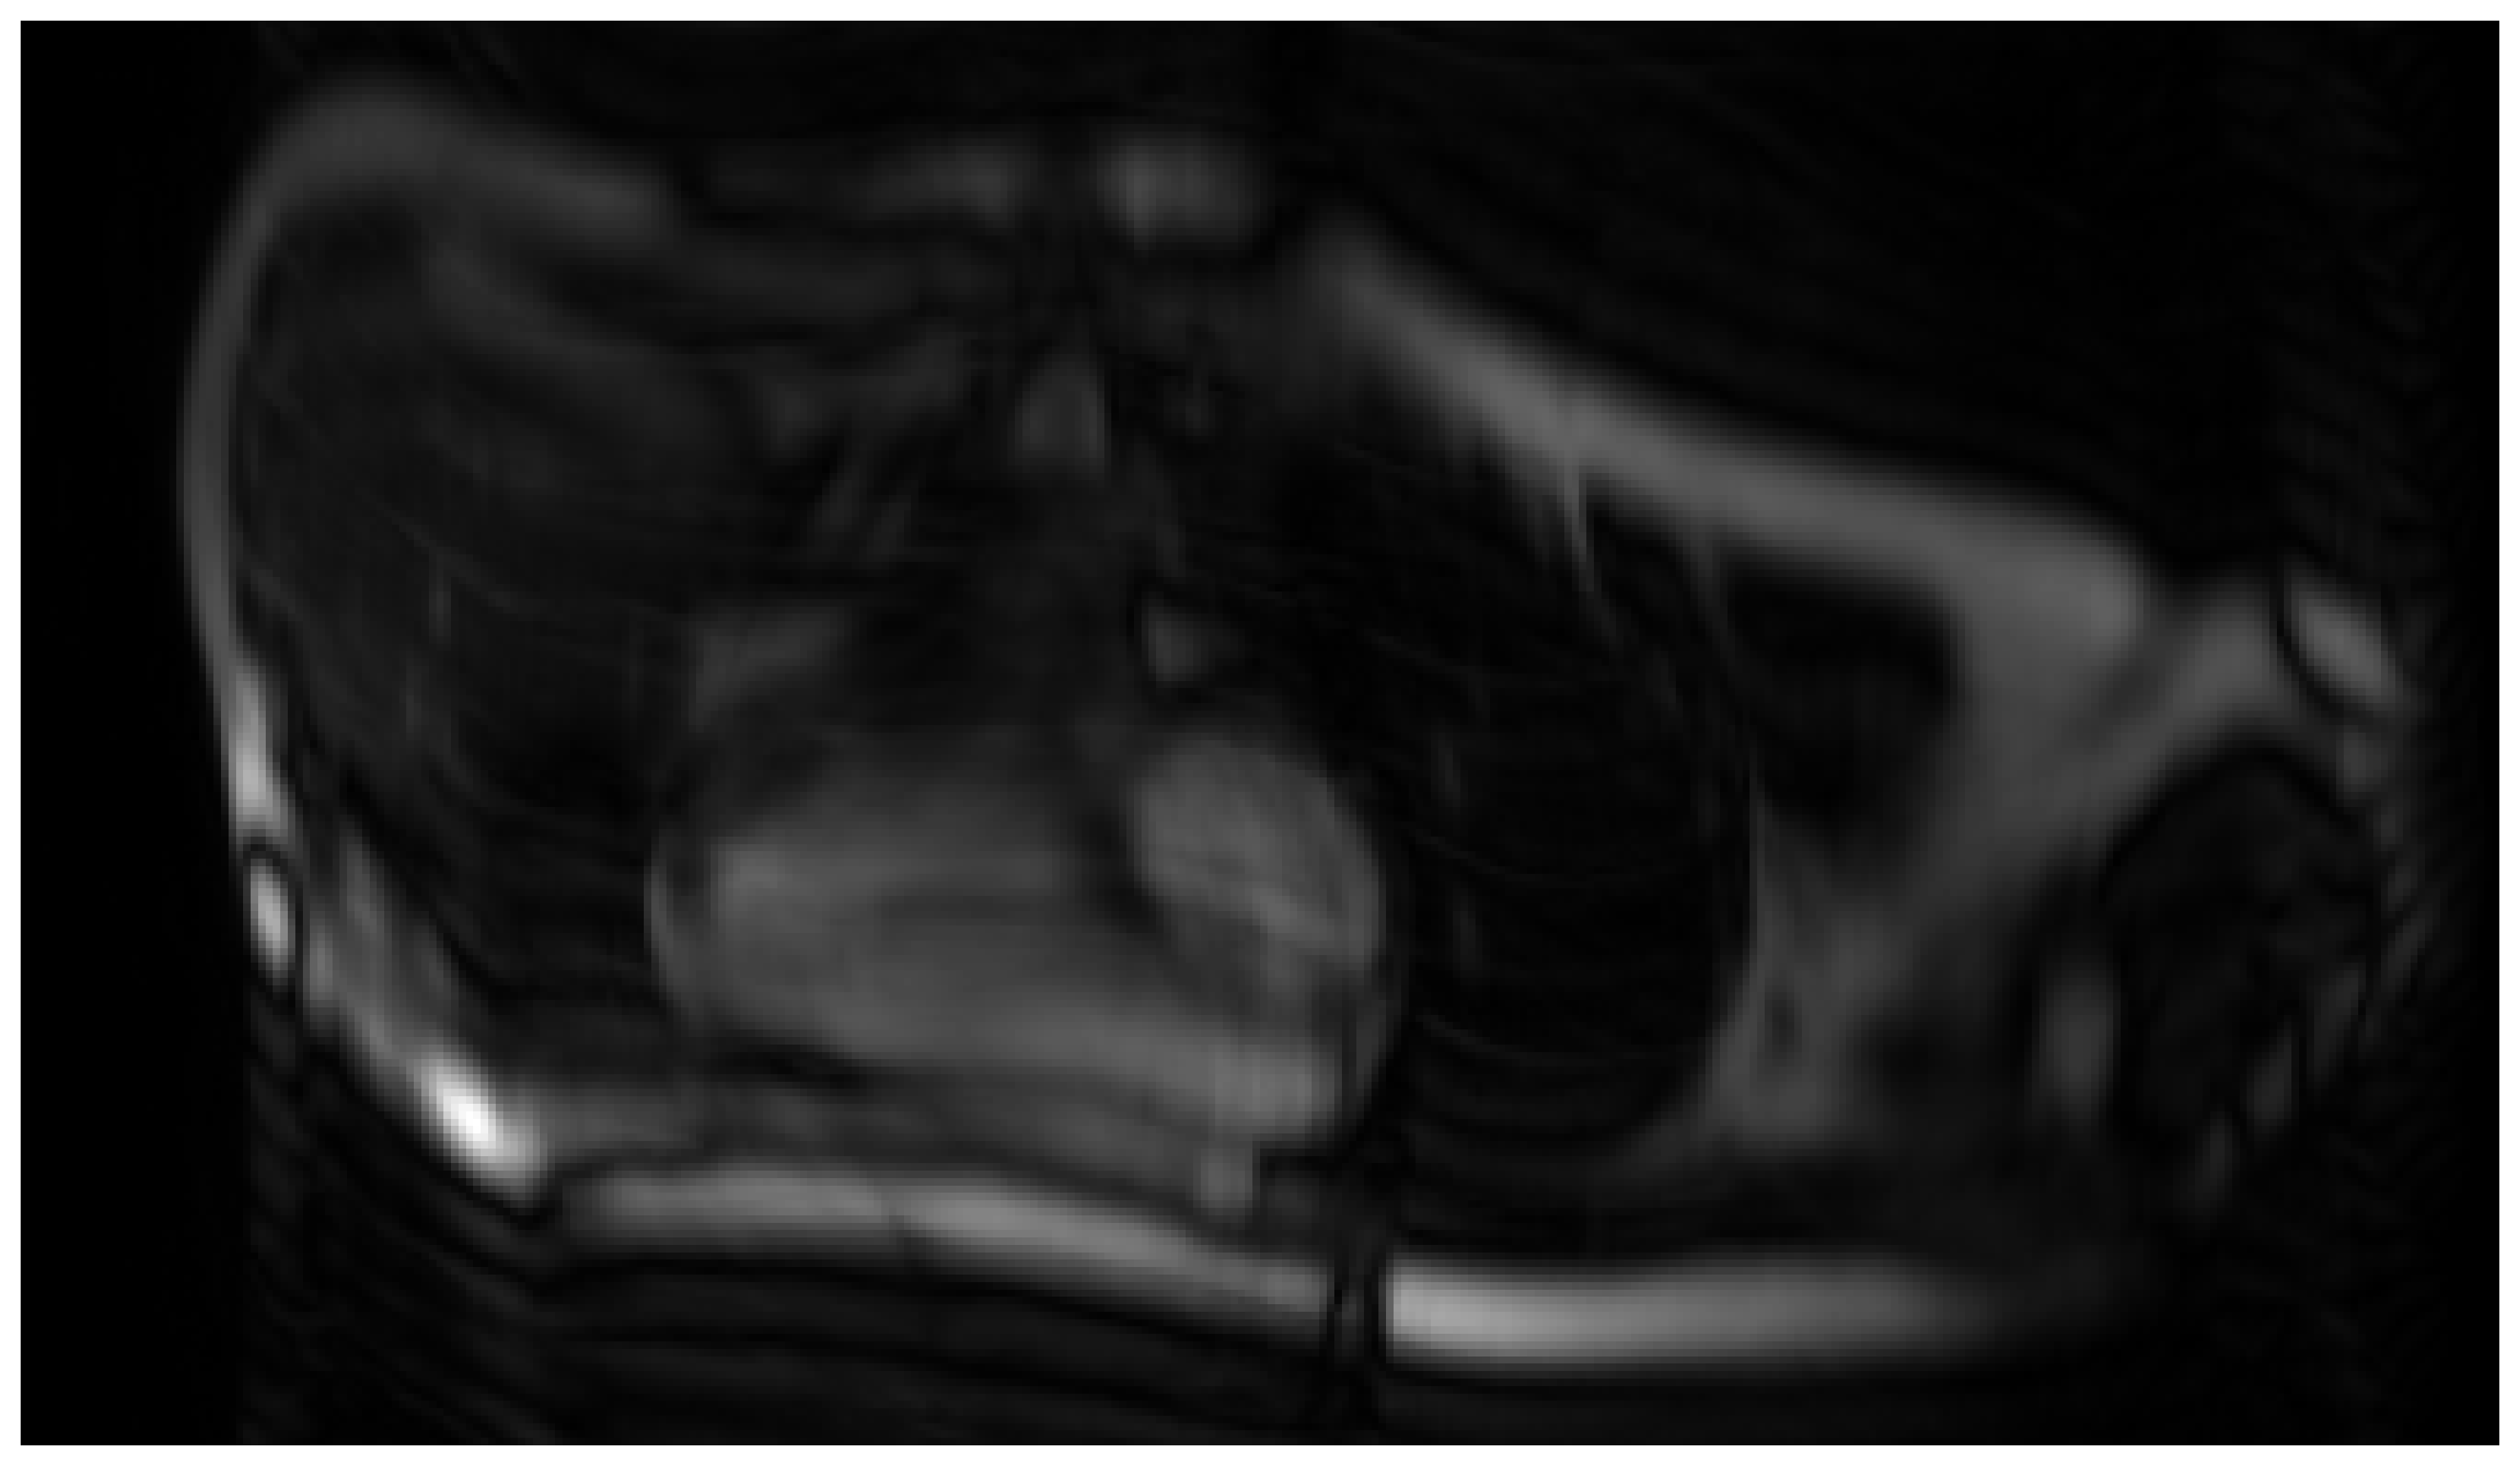
\includegraphics[width=\textwidth]{./Images/LungMotion4.png}
    		%\caption{Second subfigure.}
    		\label{fig:LungMotion4}
	\end{subfigure}
	\caption{$L=4$ images with simulated lung motion for the same cardiac frame (background was cropped out).}
	\label{fig:LungMotion}
\end{figure}


\section{Experiments} \label{Sec:Experiments}
In the following chapter the different experiments that were conducted are described and explained. 
%First was frame-to-frame registration on cardiac data from the \emph{CMRxRecon} dataset to lay the basis for later experiments with a motion-correcting reconstruction pipeline.
First, experiments were conducted on the \emph{ACDC} dataset to find the optimal parameters for our model using ground truth segmentations. Then a motion-compensated reconstruction pipeline was used as an downstream task on the \emph{CMRxRecon} dataset.


\subsection{Ablation Studies and Parameter Tests} \label{SubSec:ParameterTestsACDC}
As the evaluation on the \emph{CMRxRecon} dataset is limited to image similarity measures, further testing was done on the \emph{ACDC} dataset which contains cardiac data with segmentations. These can be used to better evaluate the registration performance by using e.g. the Dice score. The tests include comparisons between \emph{Fourier-Net}, \emph{Fourier-Net+} and \emph{4xFourier-Net}, parameter tests for the starting channel size, FT crop size as well as comparisons with VoxelMorphs and dense versions of the three networks.


\subsubsection{Fourier-Net versus Fourier-Net+} \label{SubSubSec:Fourier-NetvsFourier-Net+}
First, \emph{Fourier-Net}, \emph{Fourier-Net+} and \emph{4xFourier-Net}, as introduced in sections~\ref{SubSec:Fourier-Net} and~\ref{SubSec:Fourier-Net+}, are compared using both baseline and diffeomorphic versions. Additionally, network versions creating dense instead of band-limited displacements were used for comparison. The registration performance was evaluated on the test set using the percentage of Dice scores calculated with and without the background label, percentage of SSIM, MSE multiplied by $10^{-3}$ (denoted by m for milli) and the percentage of negative Jacobian determinant of deformation. The mean inference time on the GPU (NVIDIA GeForce RTX 2080 Ti) together with memory consumption for each model are also added to the comparison with the latter containing number of trainable model parameters, mult-add operations (in millions or billion as denoted by M or G) and the total memory in Megabyte (MB). The latter is only given for the normal versions as the diffeomorphic version require the same amount of memory as well as the baseline dense versions. The first network was trained for a maximum of 15 epochs with early stopping activating after 3 epochs without improvement of the validation Dice score. The other variants were than trained with the same number of epochs, which worked out to be only 6 epochs due to the large training set in the experiments without any data augmentation. All networks were trained on the fully sampled \emph{ACDC} data with MSE as the similarity loss, a channel size of 8, learning rate of 0.0001 and $\lambda=0.01$. \emph{Fourier-Net+} and \emph{4xFourier-Net} used a FT crop size of $48 \times 48$ for these experiments. All of these parameters were constant for the diffeomorphic and dense versions of the networks. The results can be found in section~\ref{SubSec:ResultsFourier-NetvsFourier-Net+ACDC}.


\subsubsection{Starting Channel Size} \label{SubSubSec:StartingChannelsACDC}
Next, the impact of the starting channels (see section~\ref{SubSec:Fourier-Net}) on the \emph{ACDC} data was examined as these dictate the number of features that the network uses. For this, \emph{Fourier-Net+} and \emph{4xFourier-Net+} was trained with MSE-loss, a learning rate of $0.0001$, $\lambda = 0.01$, FT crop of $48 \times 48$ and no diffeomorphic transform. The experiments were again only conducted on the fully sampled data. Four different channel sizes were used for training: $8$, $16$, $32$ and $64$. The first network variant was trained with early stopping, which ended at 6 epochs. For better comparability, the other network variants were also trained with the same number of epochs. The metrics from the previous experiment were again used. The results can be found in section~\ref{SubSec:ResultsStartingChannelsACDC}.


\subsubsection{Fourier-Transform Crop Size} \label{SubSubSec:FTCropSize}
The FT crop size, used for compressing the input images, is a parameter specific to \emph{Fourier-Net+} and \emph{4xFourier-Net+}. Four different sizes of the FT crop were analyzed: $80 \times 168$, $40 \times 84$, $48 \times 48$ and $24 \times 24$. A larger crop would obviously compress the images less, thus leading to less efficiency, however, a very small crop, while very efficient, might lose some of the image details leading to a decrease in performance. The experiments were again only conducted on the fully sampled data as one would expect similar results on subsampled data. The network variants were trained with MSE as the similarity loss, a channel size of 8, learning rate of 0.0001 and $\lambda=0.01$. Again, the networks were trained for only 5 epochs, as this is were the first model ended training due to early stopping. The registration performance was evaluated on the test set using the same metrics as before. The results can be found in section~\ref{SubSec:ResultsFTCropSize}.


\subsubsection{Comparison with VoxelMorph} \label{SubSubSec:ComparisonVoxelMorph}
After finding parameters which optimize registration performance while trying to minimize memory consumption, a comparison to another commonly used registration network was made. For this, a diffeomorphic version~\cite{VoxelMorphDiff} of the well known \emph{VoxelMorph}~\cite{Voxelmorph} was used with integration steps $T=7$. It was trained with the default number of layers, MSE as the similarity loss, a learning rate of 0.0001, $\lambda=0.01$. It provides a dense displacement field to align the image pair. For comparison \emph{Fourier-Net}, \emph{Fourier-Net+} and \emph{4xFourier-Net+} were trained for 6 epochs with MSE as the similarity loss, a channel size of 16, learning rate of 0.0001 and $\lambda=0.01$ as well as a FT crop size of $48 \times 48$, which provide a good balance of performance and memory imprint for the networks. To evaluate registration performance the same metrics as before were used. All networks were trained on the fully sampled \emph{ACDC} data and the results can be seen in section~\ref{SubSec:ResultsComparisonVoxelMorph}.


\subsubsection{Dense Displacement on Accelerated Data} \label{SubSubSec:DenseDisplacementAcc}
The difference between a dense displacement field and a band-limited one was already explored in a previous section, but only on fully sampled, not accelerated data. Potential performance changes on the latter were investigated in theses tests with the hypothesis that the network variants with the dense displacement will perform worse than the variants with the band-limited displacement field for strongly subsampled data. This expectation stems from the fact that frequencies outside the center region of the k-space are dropped for the accelerated data thus reducing the advantage of the dense displacement in comparison to the band-limited (i.e. center-cropped) displacement. The tests again included \emph{Fourier-Net}, \emph{Fourier-Net+} and \emph{4xFourier-Net+}, which were all trained for 6 epochs with MSE as the similarity loss, a channel size of 16, $48 \times 48$ FT crop, learning rate of 0.0001 and $\lambda=0.01$. The registration performance was evaluated using the same metrics as before. The results can be seen in section~\ref{SubSec:ResultsDenseDisplacementAcc}.

\subsection{Registration Performance on Subsampled Data} \label{SubSubSec:ComparisonSubsampling}
After comparing \emph{Fourier-Net}, \emph{Fourier-Net+} and \emph{4xFourier-Net+} with both dense and band-limited displacement fields as well as another comparison with \emph{VoxelMorph} on fully sampled data an extension to subsampled data needs to be made. For this \emph{Fourier-Net}, \emph{Fourier-Net+} and \emph{4xFourier-Net+} were compared to a baseline consisting of the unaligned test image pairs as well as \emph{NiftyReg}~\cite{NiftiReg}, a traditional registration algorithm, and \emph{VoxelMorph}~\cite{Voxelmorph}, a dense registration network.\\
\emph{Fourier-Net}, \emph{Fourier-Net+} and \emph{4xFourier-Net+} were trained for 6 epochs with MSE as the unsupervised similarity loss, a channel size of 16, learning rate of 0.0001 and $\lambda=0.01$ as well as a FT crop size of $48 \times 48$ for all subsampling data. VoxelMorph was trained with default layers and MSE as the similarity loss, a learning rate of 0.0001 and $\lambda=0.01$. Three subsamplings $R=4$, $R=8$ and $R=10$ were tested. For reference, the data for the fully sampled data ($R=0$) is also provided. The registration performance of all methods was evaluated on the test set using the Dice score (with and without the background label), SSIM and MSE. All times are computed on CPU for better comparability as \emph{NiftyReg} currently only works on CPU as the GPU capable versions were deprecated and the other networks would gain an unfair time advantage when ran on GPU. The baseline has no time associated as it only denotes the metrics on the test data before registration. The results are provided in section~\ref{SubSec:ResultsComparisonSubsampling}.


\subsection{Motion-Compensated Reconstruction Pipeline} \label{SubSec:IntegrationMotion-CompensatedReconstructionPipeline}
After multiple ablation studies and parameter tests to find optimal network parameters, a downstream experiment is conducted to show the usability of the networks in real-world applications. For this a motion-compensated reconstruction pipeline was chosen where the network can be used to compensate the motion-corrupted data. As the \emph{ACDC} dataset only contains already reconstructed images, the next tests were all conducted on the \emph{CMRxRecon} dataset.\\
As discussed in section~\ref{SubSec:Motion-CompensatedReconstruction}, neural networks can be used in motion-compensated MRI reconstruction pipelines for either the reconstruction or the motion-compensation. As \emph{Fourier-Net}, \emph{Fourier-Net+} and \emph{4xFourier-Net+} were already trained for frame-to-frame registration, they could be easily used for the latter. ESPIRiT~\cite{ESPIRiT} was used to simulate the coil sensitivity maps needed for a SENSE-type reconstruction from the provided k-space data using an eigenvalue decomposition~\cite{ESPIRiT}. For the SENSE~\cite{SENSE1} reconstruction, an iterative conjugate gradient algorithm was used. This made the pipeline very memory effective as \emph{Fourier-Net+} is a lightweight network. Two experiments were conducted on the \emph{CMRxRecon} dataset as it provides the needed k-space data (both fully sampled and accelerated) as well as the subsampling masks required for reconstruction. However, the cardiac scans only show a small amount of movement between frames due to cardiac movement no larger movement of e.g. the lung. Thus, the input images were further motion-corrupted as the cardiac motion present was deemed not severe enough. This process is detailed in section~\ref{SubSec:SimulatedMotion}. An overview of this augmentation incorporated into the reconstruction pipeline can be seen in Figure~\ref{fig:GeneralReconstructionPipeline}. \emph{Fourier-Net}, \emph{Fourier-Net+} and \emph{4xFourier-Net+} have been pre-trained on image reconstructed from this data via an iFT for frame-to-frame registration using the optimal settings obtained in section~\ref{SubSec:ParameterTestsACDC} (MSE-loss, 16 channels, $48 \times 48$ FT crop, learning rate 0.0001, $\lambda=0.01$). As the \emph{CMRxRecon} dataset does not include segmentations for Dice calculation, image similarity metrics need to be utilized. For this, SSIM and MSE were used again, however, the PSNR (see section~\ref{SubSec:NetworkTrainingAndTesting}) and HaarPSI~\cite{HaarPSI} were also added. For comparison \emph{VoxelMorph} was used. The results can be seen in section~\ref{Sec:ResultsIntegrationMotion-CompensatedReconstructionPipeline}.


% general reconstruction pipeline with synthetic motion-corrupted 
\begin{figure}[h] %tpb
	\centering
	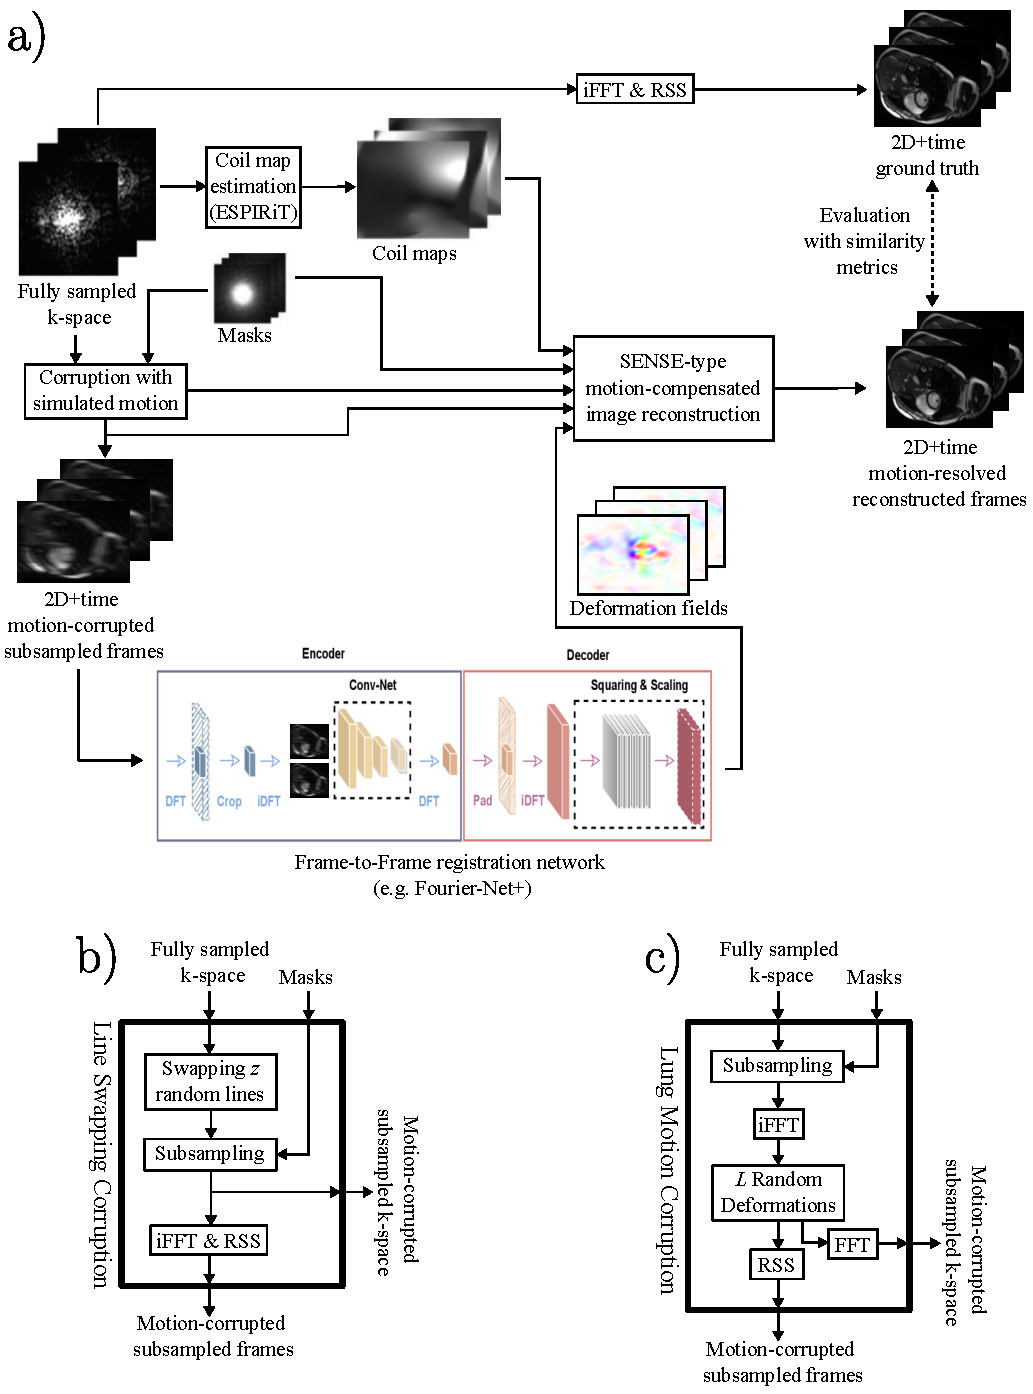
\includegraphics[width=\textwidth]{./Images/GeneralReconstructionPipeline.pdf} 
	\caption{Overview of the generalized reconstruction pipeline in a) using \emph{Fourier-Net+} as a registration network (Figure inspired by~\cite{Kuestner2022}). The k-space data is corrupted with synthetic motion, either through swapping $z$ random line (steps shown in b) or by via $L$ random deformation frames to simulate lung motion (shown in c)).}
	\label{fig:GeneralReconstructionPipeline}
\end{figure}

%%%%%%%%%%%%%
%% Results %%
%%%%%%%%%%%%%

\chapter{Results} \label{Ch:Results}
In this chapter, the results for the experiment described in section~\ref{Sec:Experiments} are reported. This includes ablation studies, parameter tests and registration performance assessment on the \emph{ACDC} dataset as well as a motion-compensated reconstruction pipeline on the \emph{CMRxRecon} dataset.
 
\section{Ablation Studies and Parameter Tests} \label{Sec:ResultsParameterTestsACDC}
In this section, the results for the ablation studies and parameter tests are described in section~\ref{SubSec:ParameterTestsACDC} are presented.

\subsection{Fourier-Net versus Fourier-Net+} \label{SubSec:ResultsFourier-NetvsFourier-Net+ACDC}
First, \emph{Fourier-Net}, \emph{Fourier-Net+} and \emph{4xFourier-Net} were compared as described in section~\ref{SubSubSec:Fourier-NetvsFourier-Net+}. The results can be seen in Table~\ref{tab:Fourier-NetvsFourier-Net+ACDC}. For the dense displacement variants, the diffeomorphic transform increases the Dice score (with and without the background label) slightly for \emph{Fourier-Net} and \emph{4xFourier-Net}, but decreases for \emph{Fourier-Net+}. The SSIM decreases for all models slightly, while the MSE remains unaffected. The percentage of non-positive Jacobian determinants is lower for the diffeomorphic variants. Times for the baseline and diffeomorphic versions are similar with the \emph{Fourier-Net} being faster without the diffeomorphism by 1.13~ms, while \emph{Fourier-Net+} and \emph{4xFourier-Net} are faster with the diffeomorphism by 3.28~ms and 1.56~ms respectively. \\
The results for the band-limited versions are very similar with \emph{Fourier-Net} and \emph{Fourier-Net+} having a lower Dice (with background) with the diffeomorphism, while \emph{4xFourier-Net} increases by almost 2$\%$. When excluding the background label \emph{Fourier-Net} is again slightly worse, but \emph{Fourier-Net+} and \emph{4xFourier-Net} both improve, the latter with almost 3$\%$ Dice more than the baseline version. The SSIM values are slightly lower for \emph{Fourier-Net} and \emph{Fourier-Net+} with the diffeomorphism, but again higher for \emph{4xFourier-Net}. The MSE is slightly lower for \emph{Fourier-Net} and \emph{4xFourier-Net}, but slightly higher for \emph{Fourier-Net+}. The percentage of non-positive Jabobian determinants again decreases for the diffeomorphic variants. The times again vary slightly with \emph{Fourier-Net} and \emph{Fourier-Net+} being slower by 0.5~ms and 6.26~ms, while \emph{4xFourier-Net} is a lot faster with 14.68~ms difference.\\
Now to the difference between the dense and band-limited displacements. Overall, the dense displacement versions have a higher Dice score for all models both with and without the background label.  The dense displacements also have better SSIM and MSE metrics, however the difference is not quite as large as with the Dice scores.  Only the percentage of non-positive Jabobian determinants is notably lower for the band-limited displacement. In terms of inference time, the dense displacement variants are slightly faster despite having a larger encoder, however all of the models are in the milliseconds (7~ms up to 33.5~ms). Last but not least, the memory consumption needs to be addressed. The dense displacment variants have a larger encoder, as discussed before, and thus have far more parameters, especially for the more optimized \emph{Fourier-Net+} and \emph{4xFourier-Net} (about 5 times more). The number of Mult-Adds and the amount of total memory are more than doubled (almost tripled for \emph{4xFourier-Net}) for the dense displacement versions compared to those with a band-limited displacement across all models.

\begin{table}[h] %htpb
	%\scriptsize
	\centering
	\caption{Results for the \emph{Fourier-Net versus Fourier-Net+} experiment. The networks are compared using both dense and band-limited displacement fields as well as diffeomorphic transforms on the fully sampled \emph{ACDC} test data.}
	\label{tab:Fourier-NetvsFourier-Net+ACDC}
	\begin{tabularx}{\textwidth}{Y Y Y Y Y} 
		\toprule
		\multirow{2}{*}{Metrics} & \multicolumn{3}{c}{Dense Displacement} \\
		\cmidrule(lr){2-4} 
		 & Fourier-Net & Fourier-Net+ & 4xFourier-Net+\\	
		\midrule
		$\%$ Dice $\uparrow$ & $78.22 \pm 13.84$ & $78.43 \pm 13.96$ & \textbf{79.34} $\pm$ \textbf{14.03}\\
		$\%$ Dice* $\uparrow$ & $71.03 \pm 18.87$ & $70.50 \pm 19.17$ & \textbf{72.02} $\pm$ \textbf{18.94} \\
		$\%$ SSIM $\uparrow$ & \textbf{91.92} $\pm$ \textbf{3.32} & $89.09 \pm 4.10$ & $89.65 \pm 3.85$\\
		MSE (m) $\downarrow$ & \textbf{0.09} $\pm$ \textbf{0.06} & $0.17 \pm 0.13$ & $0.15 \pm 0.12$ \\
		$\% \, |J_{\phi}|\leq0 \downarrow$ & $0.53 \pm 0.52$ & $0.32 \pm 0.55$ & \textbf{0.04} $\pm$ \textbf{0.09} \\
		Time [ms] $\downarrow$  & \textbf{7.03} 	& 10.74 	& 21.89 \\
		\midrule
		 & \mbox{Diff-Fourier-Net} & \mbox{Diff-Fourier-Net+} & \mbox{Diff-4xFourier-Net+}\\		
		\midrule
		$\%$ Dice $\uparrow$ & $78.56 \pm 14.13$ & $77.88 \pm 13.81$ & \textbf{79.49} $\pm$ \textbf{14.26}\\
		$\%$ Dice* $\uparrow$ & $71.31 \pm 19.13$ & $70.19 \pm 18.82$ & \textbf{72.12} $\pm$ \textbf{19.33} \\
		$\%$ SSIM $\uparrow$ & \textbf{91.79} $\pm$ \textbf{3.38} & $89.08 \pm 4.10$ & $89.62 \pm 3.98$\\
		MSE (m) $\downarrow$ & \textbf{0.09} $\pm$ \textbf{0.06} & $0.16 \pm 0.13$ & $0.15 \pm 0.12$ \\
		$\% \, |J_{\phi}|\leq0 \downarrow$ & $0.03 \pm 0.06$ & $0.00 \pm 0.00$ & $0.00 \pm 0.00$ \\
		Time [ms] $\downarrow$  & 8.16  & \textbf{7.46} & 20.33 \\
		\midrule
		Parameters $\downarrow$ & 645,216 & \textbf{380,470} & 1,521,880 \\
		Mult-Adds (G) $\downarrow$ & 1.12  	& \textbf{0.04} 	& 0.18 \\
		Memory [MB] $\downarrow$ & 97.63   & \textbf{5.81} 	& 21.90 \\
		\bottomrule
	\end{tabularx}
\end{table}
% split table to fit better onto the pages
\begin{table}[H]		
	\centering
	\begin{tabularx}{\textwidth}{Y Y Y Y Y}
		\toprule	
		\multirow{2}{*}{Metrics} & \multicolumn{3}{c}{Band-limited Displacement} \\
		\cmidrule(lr){2-4} 
		 & Fourier-Net & Fourier-Net+ & 4xFourier-Net+\\		
		\midrule
		$\%$ Dice $\uparrow$ & \textbf{77.95} $\pm$ \textbf{14.71} & $75.35 \pm 14.28$ & $76.59 \pm 14.84$\\
		$\%$ Dice* $\uparrow$ & \textbf{69.96} $\pm$ \textbf{21.55} & $64.74 \pm 21.12$ & $66.82 \pm 21.55$ \\
		$\%$ SSIM $\uparrow$ & \textbf{91.35} $\pm$ \textbf{3.51} & $88.42 \pm 3.94$ & $88.59 \pm 4.23$\\
		MSE (m) $\downarrow$ & \textbf{1.00} $\pm$ \textbf{0.71} & $2.06 \pm 1.54$ & $1.92 \pm 1.46$ \\
		$\% \, |J_{\phi}|\leq0 \downarrow$ & $0.36 \pm 0.38$ & $0.13 \pm 0.35$ & \textbf{0.03} $\pm$ \textbf{0.12} \\
		Time [ms] $\downarrow$ & \textbf{14.46} & \textbf{14.46} & 33.49 \\
		\midrule
		 & \mbox{Diff-Fourier-Net} & \mbox{Diff-Fourier-Net+} & \mbox{Diff-4xFourier-Net+}\\		
		\midrule
		$\%$ Dice $\uparrow$ & $77.93 \pm 14.93$ & $75.17 \pm 13.43$ & \textbf{78.20} $\pm$ \textbf{14.01}\\
		$\%$ Dice* $\uparrow$ & \textbf{69.91} $\pm$ \textbf{21.99} & $65.67 \pm 18.61$ & $69.61 \pm 19.11$ \\
		$\%$ SSIM $\uparrow$ & \textbf{91.24} $\pm$ \textbf{3.56} & $87.81 \pm 3.94$ & $88.81 \pm 4.13$\\
		MSE (m) $\downarrow$ & \textbf{0.98} $\pm$ \textbf{0.67} & $2.29 \pm 1.61$ & $1.85 \pm 1.41$ \\
		$\% \, |J_{\phi}|\leq0 \downarrow$ & $0.01 \pm 0.03$ & \textbf{0.00} $\pm$ \textbf{0.00} & \textbf{0.00} $\pm$ \textbf{0.00} \\
		Time [ms] $\downarrow$ 	  & \textbf{14.96}  & 20.72 & 18.81 \\
		\midrule
		Parameters $\downarrow$    & 434,519 & \textbf{75,429} & 301,716 \\
		Mult-Adds (M) $\downarrow$ & 595.04  & \textbf{10.98}  & 43.91 \\
		Memory [MB] $\downarrow$   & 44.69   & \textbf{2.25}   & 7.66 \\
		\bottomrule
	\end{tabularx}
\end{table}


\subsection{Starting Channel Size} \label{SubSec:ResultsStartingChannelsACDC}
Next, the impact of the starting channel size was examined as explained in section~\ref{SubSubSec:StartingChannelsACDC}. The results can be seen in Table~\ref{tab:StartingChannelsFourierNet+ACDC}. The Dice (with and without the background label) increased for both \emph{Fourier-Net+} and \emph{4xFourier-Net+} for larger channel sizes. A marginal increase in SSIM and MSE was observed, while the percentage of non-positive Jabobian determinants decreased. The inference time is not heavily impacted by channel size as the times remain very similar for all sizes. Overall, \emph{4xFourier-Net+} is slower than \emph{Fourier-Net+} by roughly a factor of 3 to 4. The number of parameters drastically increases with starting size leading to an increase in Mult-Add and thus overall memory. As \emph{4xFourier-Net+} is just a cascaded version of \emph{Fourier-Net+} a channel size of 16 for the latter is about the same as channel size~8 for the cascaded version and so on. This can also be seen in the direct comparison between \emph{Fourier-Net+} and \emph{4xFourier-Net+}, where the latter has a better performance, but also needs more memory. While an increase of channel size also increases performance in terms of Dice (with the background label) by $0.36\%$, $0.43\%$ and $0.41\%$ for the latter, which is quite consistent, it can be observed that an increase of channel size for \emph{Fourier-Net+} has an bigger impact at the beginning ($1.38\%$, $0.78\%$ and $0.15\%$) and fades towards larger channels sizes. This effect can also be seen when excluding the background label ($0.69\%$, $0.78\%$ and $0.42\%$ for \emph{4xFourier-Net+} compared to $2.16\%$, $1.09\%$ and $0.10\%$ for \emph{Fourier-Net+}), but is less pronounced for the SSIM and MSE. Note that all versions of \emph{Fourier-Net+} and \emph{4xFourier-Net+} are smaller in terms of total memory than \emph{Fourier-Net} with channel size~8 (44.69 MB), except for \emph{4xFourier-Net+} with channel size~64.

\begin{table}[h] %tpb
	%\scriptsize
	\centering
	\caption{Results for the different starting channel sizes of \emph{Fourier-Net+} and \emph{4xFourier-Net+} on the fully sampled \emph{ACDC} test data.}
	\label{tab:StartingChannelsFourierNet+ACDC}
	\begin{tabularx}{\textwidth}{Y Y Y Y Y}
		\toprule
		\multirow{2}{*}{Metrics} & \multicolumn{4}{c}{Starting Channels - Fourier-Net+} \\
		\cmidrule(lr){2-5}
		 & 8 & 16 & 32 & 64 \\		
		\midrule
		$\%$ Dice $\uparrow$ & $75.50 \pm 13.79$ & $76.88 \pm 13.86$ & $77.66 \pm 13.60$ & \mbox{\textbf{77.81} $\pm$ \textbf{13.76}} \\
		$\%$ Dice* $\uparrow$ & $65.70 \pm 18.96$ & $67.86 \pm 19.06$ & $68.95 \pm 18.65$ & \mbox{\textbf{69.05} $\pm$ \textbf{18.80}} \\
		$\%$ SSIM $\uparrow$ & $88.05 \pm 3.89$ & $88.67 \pm 3.88$ & $88.83 \pm 3.83$ & \textbf{89.02} $\pm$ \textbf{3.67} \\
		MSE (m) $\downarrow$ & $0.22 \pm 0.16$ & $0.20 \pm 0.15$ & \textbf{0.19} $\pm$ \textbf{0.15} & \textbf{0.19} $\pm$ \textbf{0.15} \\
		$\% \, |J_{\phi}|\leq0 \downarrow$ & $0.07 \pm 0.25$ & $0.04 \pm 0.14$ & $0.01 \pm 0.04$ & \textbf{0.00} $\pm$ \textbf{0.03} \\
		Time [ms] $\downarrow$ 	  & \textbf{7.18} & 7.77 & 7.99 & 7.79 \\
		Parameters  $\downarrow$	  & \textbf{75,429} 	& 300,477 	& 1,199,469 	& 4,793,037 \\
		\mbox{Mult-Adds (M) $\downarrow$}  & \textbf{10.98} 	& 42.89 		& 169.54 	& 674.10 \\
		\mbox{Memory [MB] $\downarrow$} 	  & \textbf{2.25} 	& 4.64 		& 11.22 		& 31.57 \\
		\midrule		
		\multirow{2}{*}{Metrics} & \multicolumn{4}{c}{Starting Channels - 4xFourier-Net+} \\
		\cmidrule(lr){2-5} 
		 & 8 & 16 & 32 & 64 \\		
		\midrule
		$\%$ Dice $\uparrow$ & $77.54 \pm 13.73$ & $77.90 \pm 13.92$ & $78.33 \pm 14.14$ & \mbox{\textbf{78.74} $\pm$ \textbf{13.91}} \\
		$\%$ Dice* $\uparrow$ & $68.52 \pm 18.62$ & $69.21 \pm 19.02$ & $69.99 \pm 19.21$ & \mbox{\textbf{70.41} $\pm$ \textbf{19.02}} \\
		$\%$ SSIM $\uparrow$ & $88.70 \pm 4.17$ & $88.89 \pm 4.05$ & $89.08 \pm 4.01$ & \textbf{89.29} $\pm$ \textbf{3.74} \\
		MSE (m) $\downarrow$ & $0.19 \pm 0.14$ & $0.19 \pm 0.14$ & \textbf{0.18} $\pm$ \textbf{0.14} & \textbf{0.18} $\pm$ \textbf{0.14} \\
		$\% \, |J_{\phi}|\leq0 \downarrow$ & $0.02 \pm 0.07$ & $0.01 \pm 0.04$ & $0.01 \pm 0.05$ & \textbf{0.00} $\pm$ \textbf{0.00} \\
		Time [ms] $\downarrow$ 	  & 30.13 	& \textbf{24.61} 	& 29.65 	& 27.73 \\
		Parameters $\downarrow$ 	  & \textbf{301,716} 	& 1,201,908 	& 4,797,876 	& 19,172,148 \\
		\mbox{Mult-Adds (G) $\downarrow$} & \textbf{0.04} 	& 0.17 		& 0.68 		& 2.70 \\
		\mbox{Memory [MB]  $\downarrow$}	  & \textbf{7.66} 	& 17.23 		& 43.56 		& 124.94 \\
		\bottomrule
	\end{tabularx}
\end{table}


\subsection{Fourier-Transform Crop Size} \label{SubSec:ResultsFTCropSize}
The results for the FT crop size experiment, as described in section~\ref{SubSubSec:FTCropSize}, can be seen in Table~\ref{tab:FTCropSize}. The Dice score, both with and without the background label, decreases drastically with a smaller crop size. The SSIM and MSE values also get worse (SSIM decreases, MSE increases), however, the percentage of non-positive Jabobian determinants decreases for smaller crop sizes. It should be noted that the crop size of $48 \times 48$ is an outlier in this regard breaking the trend with a higher percentage as $40 \times 84$. The inference time also decreases slightly with a smaller crop size, although this is quite noisy as the time from $80 \times 168$ to $40 \times 84$ is halved for \emph{Fourier-Net+}, but the time needed for $48 \times 48$ and $24 \times 24$ increases again very slightly. For \emph{4xFourier-Net+} the time decrease for all smaller crop sizes, except for $24 \times 24$. The number of parameters does not change for different crop sizes as the networks themselves do not change, however the number of Mult-Adds and the total memory still change with the image size. Both decrease with a larger crop size as the image gets smaller. This effect is again not linear as a reduction in image size yields a larger reduction in memory going from $80 \times 168$ to $40 \times 84$ than from $48 \times 48$ to $24 \times 24$. 

\begin{table}[h] %tpb
	%\scriptsize
	\centering
	\caption{Results for four different FT crop sizes for \emph{Fourier-Net+} and \emph{4xFourier-Net+} examined on the fully sampled \emph{ACDC} test data.}
	\label{tab:FTCropSize}
	\begin{tabularx}{\textwidth}{Y Y Y Y Y} 
		\toprule
		\multirow{2}{*}{Metrics} & \multicolumn{4}{c}{FT crop size - Fourier-Net+} \\
		\cmidrule(lr){2-5}
		 & $80 \times 168$ & $40 \times 84$ & $48 \times 48$ & $24 \times 24$ \\		
		\midrule
		$\%$ Dice $\uparrow$ & \mbox{\textbf{78.24} $\pm$ \textbf{14.43}} & $76.61 \pm 13.90$ & $75.27 \pm 13.49$ & $73.77 \pm 14.42$ \\
		$\%$ Dice* $\uparrow$ & \mbox{\textbf{70.66} $\pm$ \textbf{19.70}} & $67.60 \pm 19.24$ & $65.48 \pm 18.76$ & $63.37 \pm 20.07$ \\
		$\%$ SSIM $\uparrow$ & \textbf{89.81} $\pm$ \textbf{4.09} & $88.58 \pm 3.87$ & $87.98 \pm 3.91$ & $87.00 \pm 3.99$ \\
		MSE (m) $\downarrow$ & \textbf{0.15} $\pm$ \textbf{0.12} & $0.20 \pm 0.15$ & $0.22 \pm 0.16$ & $0.27 \pm 0.19$ \\
		$\% \, |J_{\phi}|\leq0 \downarrow$ & $0.22 \pm 0.46$ & $0.05 \pm 0.15$ & $0.09 \pm 0.25$ & \textbf{0.00} $\pm$ \textbf{0.02} \\		
		Time [ms]  $\downarrow$	  & \textbf{6.99} & 7.71 & 7.18 & 8.14 \\
		Parameters  $\downarrow$	  & 75,429 & 75,429 & 75,429 & 75,429 \\
		\mbox{Mult-Adds (M) $\downarrow$} & 64.03  & 16.37  & 10.98  & \textbf{2.74} \\
		\mbox{Memory [MB]  $\downarrow$} 	  & 9.51   & 2.97   & 2.25   & \textbf{1.12} \\
		\midrule
		\multirow{2}{*}{Metrics} & \multicolumn{4}{c}{FT crop size - 4xFourier-Net+} \\
		\cmidrule(lr){2-5}
		 & $80 \times 168$ & $40 \times 84$ & $48 \times 48$ & $24 \times 24$ \\		
		\midrule
		$\%$ Dice $\uparrow$ & \mbox{\textbf{78.12} $\pm$ \textbf{15.01}} & $77.49 \pm 14.67$ & $74.95 \pm 14.15$ & $72.58 \pm 14.67$ \\
		$\%$ Dice* $\uparrow$ & \mbox{\textbf{70.08} $\pm$ \textbf{21.92}} & $68.03 \pm 21.57$ & $64.54 \pm 20.75$ & $61.19 \pm 21.63$ \\
		$\%$ SSIM $\uparrow$ & \textbf{89.91} $\pm$ \textbf{4.01} & $89.03 \pm 3.98$ & $87.98 \pm 3.94$ & $87.02 \pm 3.95$ \\
		MSE (m) $\downarrow$ & \textbf{1.45} $\pm$ \textbf{1.11} & $1.81 \pm 1.37$ & $2.22 \pm 1.61$ & $2.64 \pm 1.84$ \\
		$\% \, |J_{\phi}|\leq0 \downarrow$ & $0.12 \pm 0.23$ & $0.03 \pm 0.15$ & $0.06 \pm 0.23$ & \textbf{0.02} $\pm$ \textbf{0.15} \\	
		Time [ms] $\downarrow$ 	 & 39.03  & 30.05  & 30.13  & \textbf{28.86} \\
		Parameters  $\downarrow$	 & 301,716 & 301,716 & 301,716 & 301,716 \\
		\mbox{Mult-Adds (M) $\downarrow$} & 256.14  & 65.50   & 43.91   & \textbf{10.98} \\
		\mbox{Memory [MB]  $\downarrow$} 	 & 36.70   & 10.54   & 7.66    & \textbf{3.15} \\
		\bottomrule
	\end{tabularx}
\end{table}

\subsection{Comparison with VoxelMorph} \label{SubSec:ResultsComparisonVoxelMorph}
Next is the comparison with \emph{VoxelMorph}, as described in section~\ref{SubSubSec:ComparisonVoxelMorph}. The results can be seen in Table~\ref{tab:CompareVoxelMorph}. \emph{VoxelMorph} has the lowest Dice score with the background label, however it does have a higher value than \emph{Fourier-Net+} for the Dice without the background label. \emph{Fourier-Net} has the highest Dice scores (both with and without the background label), followed by \emph{4xFourier-Net+}. \emph{VoxelMorph} has the best SSIM and MSE values, followed by \emph{Fourier-Net}. The percentage of non-positive Jabobian determinants for \emph{VoxelMorph} is high with $1\%$ while the other models are all under $0.25\%$. In terms of time, \emph{4xFourier-Net+} is slowest followed by \emph{VoxelMorph}, \emph{Fourier-Net+} and \emph{Fourier-Net}, although all models are very fast (less than 25~ms per image pair). The model with the least amount of parameters and Mult-Adds is \emph{VoxelMorph}, however it still requires quite a lot of memory with almost 40~MB. \emph{Fourier-Net} is the largest model in terms of model parameters, Mult-Adds and total memory (90~MB). \emph{Fourier-Net+} and \emph{4xFourier-Net+} both have a higher number of parameters and Mult-Adds, but a lower total amount of memory is needed (5~MB and 17~MB). 

\begin{table}[h] %tpb
	%\scriptsize
	\centering
	\caption{Comparison of \emph{Fourier-Net}, \emph{Fourier-Net+}, \emph{4xFourier-Net+} and \emph{VoxelMorph} with similarity metrics and memory consumption on the fully sampled \emph{ACDC} test data.}
	\label{tab:CompareVoxelMorph}
	
	\begin{tabularx}{\textwidth}{Y Y Y Y Y} 
		\toprule
		 & Fourier-Net & Fourier-Net+ & \mbox{4xFourier-Net+} & VoxelMorph \\		
		\midrule
		$\%$ Dice $\uparrow$ & \mbox{\textbf{78.31} $\pm$ \textbf{13.96}} & $76.88 \pm 13.86$ & $77.90 \pm 13.92$ & $75.84 \pm 13.46$ \\
		$\%$ Dice* $\uparrow$ & \mbox{\textbf{71.17} $\pm$ \textbf{18.99}} & $67.86 \pm 19.06$ & $69.21 \pm 19.02$ & $68.25 \pm 18.36$ \\
		$\%$ SSIM $\uparrow$ & $91.53 \pm 3.49$ & $88.67 \pm 3.88$ & $88.89 \pm 4.05$ & \textbf{93.53} $\pm$ \textbf{3.30} \\
		MSE (m) $\downarrow$ & $0.09 \pm 0.07$ & $0.20 \pm 0.15$ & $0.19 \pm 0.14$ & \textbf{0.06} $\pm$ \textbf{0.04} \\
		$\% \, |J_{\phi}|\leq0 \downarrow$ & $0.24 \pm 0.45$ & $0.02 \pm 0.14$ & \textbf{0.00} $\pm$ \textbf{0.04} & $1.00 \pm 0.57$ \\
		Time [ms] $\downarrow$ 	  & \textbf{7.58}    & 7.78 	& 24.61  	& 10.82 \\
		Parameters $\downarrow$ 	  & 1,735,447 & 300,477 	& 1,201,908 	& \textbf{84,322} \\
		\mbox{Mult-Adds (G) $\downarrow$} & 2.35      & 0.04289  & 0.17157  	& \textbf{0.00157} \\
		\mbox{Memory [MB]  $\downarrow$} 	  & 90.08     & \textbf{4.64}   	& 17.23    	& 39.04 \\
		\bottomrule
	\end{tabularx}	
\end{table}


\subsection{Dense Displacement on Accelerated Data} \label{SubSec:ResultsDenseDisplacementAcc}
The difference between a dense displacement field and a band-limited one was already explored in section~\ref{SubSec:ResultsFourier-NetvsFourier-Net+ACDC}. However, the results in Table~\ref{tab:Fourier-NetvsFourier-Net+ACDC} only include fully sampled data, not accelerated data. These new tests again included \emph{Fourier-Net}, \emph{Fourier-Net+} and \emph{4xFourier-Net+}, but are extended to subsampled data. Results for $R=4$ can be seen in Table~\ref{tab:DenseDisplacementAcc4}, $R=8$ in Table~\ref{tab:DenseDisplacementAcc8} and $R=10$ in Table~\ref{tab:DenseDisplacementAcc10}. \\
For $R=4$, the dense version of \emph{Fourier-Net}, \emph{Fourier-Net+} and \emph{4xFourier-Net+} have higher Dice scores than the band-limited versions, though the differences are less than a percent with and less than two percent without the background label. The same is true for the SSIM and MSE values with the dense versions being better. It should be noted that \emph{Fourier-Net} performs best for all the aforementioned metrics for the dense and band-limited displacements with the exception of the Dice with the background label where the band-limited \emph{4xFourier-Net+} is better. The percentage of non-positive Jabobian determinants is higher for the band-limited \emph{Fourier-Net}, while band-limited \emph{Fourier-Net+} and \emph{4xFourier-Net+} show almost no folding. 
%While this at first seems like a positive metric it can also indicate a lack of complex displacements which could explain the lower performance. 
Band-limited \emph{Fourier-Net} and \emph{Fourier-Net+} are faster (1.6~ms and 1.76~ms), likely due to the smaller network size as the encoder lack some layers compared to the dense versions, however, band-limited \emph{4xFourier-Net+} is slower than its dense counterpart by 4.93~ms. Overall, \emph{Fourier-Net+} is the fastest network for both dense and band-limited displacements.\\
For $R=8$, all band-limited networks have a lower Dice and SSIM values with a higher MSE. Band-limited \emph{4xFourier-Net+} again has the highest Dice with the background for the band-limited networks while \emph{Fourier-Net} has the highest Dice without background, SSIM and lowest MSE. While it also previously performed best for all these metrics for the dense displacements, \emph{4xFourier-Net+} now has the highest Dice scores for all dense networks. The percentage of non-positive Jabobian determinants is again higher for the band-limited \emph{Fourier-Net} compared to the dense version, while the band-limited \emph{Fourier-Net+} and \emph{4xFourier-Net+} show almost no folding. Band-limited \emph{Fourier-Net} and \emph{Fourier-Net+} are faster by 2.49~ms and 3.08~ms while \emph{4xFourier-Net+} is slower compared to its dense counterpart by 8.03~ms. For both dense and band-limited networks, \emph{Fourier-Net+} is the fastest network.\\
For $R=10$, the dense networks again have higher Dice and SSIM values compared to the band-limited versions. For the MSE, band-limited \emph{Fourier-Net} has similar values to its dense counterpart, while band-limited \emph{Fourier-Net+} and \emph{4xFourier-Net+} are again slightly higher compared to the dense versions. For the dense versions \emph{4xFourier-Net+} again has the highest Dice scores, while \emph{Fourier-Net} hast the highest SSIM value and lowest MSE value. Band-limited \emph{4xFourier-Net+} again has the highest Dice score with the background with band-limited \emph{Fourier-Net} has the highest Dice score without background, SSIM and lowest MSE. The percentage of non-positive Jabobian determinants for the band-limited \emph{Fourier-Net} is equal to the percentage of the dense version, while band-limited \emph{Fourier-Net+} and \emph{4xFourier-Net+} again show almost no folding. Band-limited \emph{Fourier-Net} is faster with 19.9~ms, although the time for dense network is probably an outlier while the band-limited version is fastest for the band-limited networks. \emph{Fourier-Net+} and \emph{4xFourier-Net+} are slower compared to their dense versions with 0.13~ms and 9.58~ms. For the dense networks, \emph{Fourier-Net+} is the fastest network.


\begin{table}[h] %tpb
	%\scriptsize
	\centering
	\caption{Results for \emph{Fourier-Net}, \emph{Fourier-Net+} and \emph{4xFourier-Net+} with both dense and band-limited displacement fields on the $R=4$ \emph{ACDC} test data.}
	\label{tab:DenseDisplacementAcc4}
	\begin{tabularx}{\textwidth}{Y Y Y Y} 
		\toprule
		\multirow{2}{*}{Metrics} & \multicolumn{3}{c}{Dense Displacement} \\
		\cmidrule(lr){2-4} 
		 & Fourier-Net & Fourier-Net+ & 4xFourier-Net+\\	
		\midrule
		$\%$ Dice $\uparrow$ & \textbf{77.37} $\pm$ \textbf{13.92} & $76.90 \pm 14.12$ & $77.35 \pm 14.04$\\
		$\%$ Dice* $\uparrow$ & \textbf{68.98} $\pm$ \textbf{19.10} & $68.39 \pm 19.30$ & $68.76 \pm 19.32$ \\
		$\%$ SSIM $\uparrow$ & \textbf{84.75} $\pm$ \textbf{7.01} & $79.79 \pm 9.76$ & $80.32 \pm 9.37$\\
		MSE (m) $\downarrow$ & \textbf{0.08} $\pm$ \textbf{0.05} & $0.15 \pm 0.12$ & $0.13 \pm 0.10$ \\
		$\% \, |J_{\phi}|\leq0 \downarrow$ & $0.16 \pm 0.19$ & $0.11 \pm 0.21$ & \textbf{0.03} $\pm$ \textbf{0.07} \\
		Time [ms] $\downarrow$ 	  & 8.49 & \textbf{8.26} & 26.33  \\
		\midrule
		\multirow{2}{*}{Metrics} & \multicolumn{3}{c}{Band-limited Displacement} \\
		\cmidrule(lr){2-4} 
		 & Fourier-Net & Fourier-Net+ & 4xFourier-Net+\\		
		\midrule
		$\%$ Dice $\uparrow$ & $76.55 \pm 13.89$ & $76.20 \pm 13.57$ & \textbf{77.23} $\pm$ \textbf{13.73}\\
		$\%$ Dice* $\uparrow$ & \textbf{67.90} $\pm$ \textbf{19.44} & $66.30 \pm 19.01$ & $67.67 \pm 18.97$ \\
		$\%$ SSIM $\uparrow$ & \textbf{82.93} $\pm$ \textbf{8.12} & $77.74 \pm 10.69$ & $77.96 \pm 10.57$\\
		MSE (m) $\downarrow$ & \textbf{0.10} $\pm$ \textbf{0.06} & $0.19 \pm 0.14$ & $0.18 \pm 0.13$ \\
		$\% \, |J_{\phi}|\leq0 \downarrow$ & $0.35 \pm 0.41$ & $0.01 \pm 0.05$ & \textbf{0.00} $\pm$ \textbf{0.02} \\
		Time [ms] $\downarrow$ 	  & 6.89  	& \textbf{6.50} 	& 31.26  \\
		\bottomrule
	\end{tabularx}
\end{table}


\begin{table}[h] %tpb
	%\scriptsize
	\centering
	\caption{Results for \emph{Fourier-Net}, \emph{Fourier-Net+} and \emph{4xFourier-Net+} with both dense and band-limited displacement fields on the $R=8$ \emph{ACDC} test data.}
	\label{tab:DenseDisplacementAcc8}
	\begin{tabularx}{\textwidth}{Y Y Y Y} 
		\toprule
		\multirow{2}{*}{Metrics} & \multicolumn{3}{c}{Dense Displacement} \\
		\cmidrule(lr){2-4} 
		 & Fourier-Net & Fourier-Net+ & 4xFourier-Net+\\	
		\midrule
		$\%$ Dice $\uparrow$ & $77.48 \pm 14.00$ & $77.30 \pm 13.72$ & \textbf{77.80} $\pm$ \textbf{14.02}\\
		$\%$ Dice* $\uparrow$ & $68.86 \pm 19.34$ & $68.39 \pm 19.15$ & \textbf{69.18} $\pm$ \textbf{19.37} \\
		$\%$ SSIM $\uparrow$ & \textbf{90.08} $\pm$ \textbf{3.05} & $87.60 \pm 3.78$ & $87.91 \pm 3.64$\\
		MSE (m) $\downarrow$ & \textbf{0.05} $\pm$ \textbf{0.04} & $0.10 \pm 0.10$ & $0.09 \pm 0.09$ \\
		$\% \, |J_{\phi}|\leq0 \downarrow$ & $0.11 \pm 0.15$ & $0.06 \pm 0.13$ & \textbf{0.02} $\pm$ \textbf{0.06} \\
		Time [ms] $\downarrow$ 	  & 11.46 & \textbf{10.79} & 38.55  \\
		\midrule
		\multirow{2}{*}{Metrics} & \multicolumn{3}{c}{Band-limited Displacement} \\
		\cmidrule(lr){2-4} 
		 & Fourier-Net & Fourier-Net+ & 4xFourier-Net+\\		
		\midrule
		$\%$ Dice $\uparrow$ & $75.52 \pm 13.69$ & $75.76 \pm 13.43$ & \textbf{76.56} $\pm$ \textbf{13.47}\\
		$\%$ Dice* $\uparrow$ & \textbf{66.86} $\pm$ \textbf{18.97} & $65.45 \pm 18.63$ & $66.81 \pm 18.77$ \\
		$\%$ SSIM $\uparrow$ & \textbf{89.51} $\pm$ \textbf{3.34} & $86.30 \pm 4.18$ & $86.29 \pm 4.23$\\
		MSE (m) $\downarrow$ & \textbf{0.06} $\pm$ \textbf{0.04} & $0.13 \pm 0.11$ & $0.13 \pm 0.11$ \\
		$\% \, |J_{\phi}|\leq0  \downarrow$ & $0.27 \pm 0.29$ & $0.03 \pm 0.11$ & \textbf{0.00} $\pm$ \textbf{0.02} \\
		Time [ms] $\downarrow$ 	  & 8.97 & \textbf{7.71} & 46.58  \\
		\bottomrule
	\end{tabularx}
\end{table}


\begin{table}[h] %tpb
	%\scriptsize
	\centering
	\caption{Results for \emph{Fourier-Net}, \emph{Fourier-Net+} and \emph{4xFourier-Net+} with both dense and band-limited displacement fields on the $R=10$ \emph{ACDC} test data.}
	\label{tab:DenseDisplacementAcc10}
	\begin{tabularx}{\textwidth}{Y Y Y Y} 
		\toprule
		\multirow{2}{*}{Metrics} & \multicolumn{3}{c}{Dense Displacement} \\
		\cmidrule(lr){2-4} 
		 & Fourier-Net & Fourier-Net+ & 4xFourier-Net+\\	
		\midrule
		$\%$ Dice $\uparrow$ & $77.39 \pm 13.89$ & $77.31 \pm 13.82$ & \textbf{77.43} $\pm$ \textbf{13.99}\\
		$\%$ Dice* $\uparrow$ & $68.86 \pm 19.27$ & $68.69 \pm 19.07$ & \textbf{68.90} $\pm$ \textbf{19.43} \\
		$\%$ SSIM $\uparrow$ & \textbf{92.92} $\pm$ \textbf{2.68} & $91.09 \pm 3.42$ & $91.33 \pm 3.29$\\
		MSE (m) $\downarrow$ & \textbf{0.05} $\pm$ \textbf{0.04} & $0.09 \pm 0.09$ & $0.08 \pm 0.09$ \\
		$\% \, |J_{\phi}|\leq0 \downarrow$ & $0.11 \pm 0.15$ & $0.06 \pm 0.11$ & \textbf{0.04} $\pm$ \textbf{0.11} \\
		Time [ms] $\downarrow$ 	  & 27.96 & \textbf{9.49} & 18.31  \\
		\midrule
		\multirow{2}{*}{Metrics} & \multicolumn{3}{c}{Band-limited Displacement} \\
		\cmidrule(lr){2-4} 
		 & Fourier-Net & Fourier-Net+ & 4xFourier-Net+\\		
		\midrule
		$\%$ Dice $\uparrow$ & $76.87 \pm 13.97$ & $76.10 \pm 13.83$ & \textbf{76.98} $\pm$ \textbf{13.57}\\
		$\%$ Dice* $\uparrow$ & \textbf{68.24} $\pm$ \textbf{19.27} & $66.27 \pm 19.20$ & $67.40 \pm 18.90$ \\
		$\%$ SSIM $\uparrow$ & \textbf{92.77} $\pm$ \textbf{2.74} & $90.32 \pm 3.29$ & $90.42 \pm 3.33$\\
		MSE (m) $\downarrow$ & \textbf{0.05} $\pm$ \textbf{0.04} & $0.12 \pm 0.12$ & $0.11 \pm 0.11$ \\
		$\% \, |J_{\phi}|\leq0 \downarrow$ & $0.11 \pm 0.15$ & $0.01 \pm 0.05$ & \textbf{0.00} $\pm$ \textbf{0.03} \\
		Time [ms] $\downarrow$ 	  & \textbf{8.06} & 9.62 & 27.89  \\
		\bottomrule
	\end{tabularx}
\end{table}
 
%\newpage
\section{Registration Performance on Subsampled Data} \label{SubSec:ResultsComparisonSubsampling}
In section~\ref{SubSec:ResultsComparisonVoxelMorph}, \emph{Fourier-Net}, \emph{Fourier-Net+} and \emph{4xFourier-Net+} were already compared to \emph{VoxelMorph}, however, these comparisons were only done on fully sampled, not accelerated data. To further add to the comparison, \emph{NiftyReg} was again used as a traditional registration algorithm. The unaligned test image pairs were treated as a baseline for the lower bound of registration performance. The results can be seen in Table~\ref{tab:ComparisonSubsamplingACDC} for fully sampled ($R=0$) and subsampled ($R=4$, $R=8$, $R=10$) \emph{ACDC} test data. Values which are worse than the baseline are marked in red, while the best results for each acceleration level and metric is highlighted with blue. All times are computed on CPU due to \emph{NiftyReg} only working on the CPU as the GPU capable versions were deprecated. Additionally, Figure~\ref{fig:Boxplots_DiceScores} shows the performance of the methods for each segmentation label (excluding the background) while Figure~\ref{fig:TestExamples} shows example images and segmentations warped by the different methods for a visual comparison.\\
For $R=0$, \emph{Fourier-Net} has the highest Dice score (both with and without the background label), closely followed by \emph{4xFourier-Net+}, while \emph{NiftyReg} performs worse than the baseline. \emph{VoxelMorph} has the highest SSIM, followed by \emph{Fourier-Net} and \emph{NiftyReg}, as well as the lowest MSE where \emph{NiftyReg} again performs worse than the baseline. \emph{NiftyReg} and \emph{4xFourier-Net+} have the lowest percentage of non-positive Jabobian determinants while \emph{VoxelMorph} has the highest value with $1\%$, thus indicating some folding. \emph{Fourier-Net} is the fastest method with under $0.1s$ per image pair, while \emph{NiftyReg} needs over $100s$ on the fully sampled data, making it the slowest by a large margin (all other methods were under $1s$).\\
For $R=4$, the registration performance decreases for all methods with \emph{NiftyReg} again performing worse than the baseline, while \emph{4xFourier-Net+} has the highest Dice score with the background label, while \emph{Fourier-Net} has the highest Dice score without the background. \emph{VoxelMorph} has the highest SSIM and lowest MSE values, followed by \emph{Fourier-Net} and \emph{NiftyReg}, with none of methods performing worse than the baseline. \emph{4xFourier-Net+} again has the lowest percentage of non-positive Jabobian determinants, closely followed by \emph{Fourier-Net+}, while \emph{VoxelMorph}, similar to the fully sampled data, has the highest value. In terms of time, \emph{NiftyReg} is again the slowest method with about $80s$, while all other methods need around $0.1s$ with \emph{Fourier-Net+} being the fastest.\\
For $R=8$, \emph{4xFourier-Net+} again has the highest Dice score with the background label, while \emph{Fourier-Net} has the highest Dice score without the background label. \emph{NiftyReg} has a lower Dice than the baseline (both with and without the background label). \emph{NiftyReg} again performs best for SSIM and MSE followed by \emph{Fourier-Net} and \emph{NiftyReg}. \emph{4xFourier-Net+} has the lowest percentage of non-positive Jabobian determinants followed by \emph{Fourier-Net+}, while \emph{VoxelMorph} again has the highest value. \emph{NiftyReg} is the slowest method, as before, with over $80s$, similar to $R=4$, while \emph{Fourier-Net+} is again the fastest despite being slightly slower than before.\\
For $R=10$, \emph{4xFourier-Net+} has the highest Dice score with the background label, while \emph{Fourier-Net} has the highest Dice score without the background. \emph{NiftyReg} again has a lower Dice score than the baseline (both with and without background label), while \emph{VoxelMorph} is the best method in terms of SSIM and MSE, followed by \emph{Fourier-Net} and \emph{NiftyReg} with no method being worse than the baseline for these metrics. \emph{4xFourier-Net+}, again, has the lowest percentage of non-positive Jabobian determinants closely followed by \emph{Fourier-Net+}, while \emph{VoxelMorph} has the highest value like before. \emph{Fourier-Net+} is again the fastest method with under $0.01s$, while \emph{NiftyReg} is again the slowest despite its best time yet with about $47s$.


\begin{table}[h] %tpb
	%\tiny
	%\scriptsize
	\footnotesize
	\centering
	\caption{Test results for \emph{NiftiReg} (NR), \emph{VoxelMorph} (VM), \emph{Fourier-Net} (F-Net), \emph{Fourier-Net+} (F-Net+) and \emph{4xFourier-Net+} (4xF-Net+) on the \emph{ACDC} test data from fully sampled ($R=0$) to $R=10$ with an unaligned baseline for comparison. The best results for each metric and subsampling are highlighted in blue, while values worse than the unaligned baseline are marked with red.}
	\label{tab:ComparisonSubsamplingACDC}
	\resizebox{\textwidth}{!}{
	\begin{tabular}{c c c c c c c c} 
		\toprule
		  & \multirow{2}{*}{Methods} & \multicolumn{6}{c}{Metrics} \\
		\cmidrule(lr){3-8} 
		  & & $\%$ DICE $\uparrow$ & $\%$ DICE* $\uparrow$ & $\%$ SSIM $\uparrow$ & MSE (m) $\downarrow$ & $\% \, |J_{\phi}|\leq0 \downarrow$ & Time [s] $\downarrow$ \\
		% Fully Sampled (R=0)
		\midrule
		\multirow{6}{*}{\rotatebox{90}{$R=0$}} & Baseline & $70.85 \pm 18.27$  & $60.35 \pm 25.24$ & $86.39 \pm 4.08$ & $0.33 \pm 0.23$ & - & -\\  
		 & NR & \textcolor{red}{$70.74 \pm 13.77$} & \textcolor{red}{$57.56 \pm 18.86$} & $91.26 \pm 3.18$ & \textcolor{red}{$1.94 \pm 1.61$} & \textcolor{blue}{$0.00 \pm 0.02$} & 122.52\\
		 & VM & $75.84 \pm 13.46$ & $68.25 \pm 18.36$ & \textcolor{blue}{$93.53 \pm 3.30$} & \textcolor{blue}{$0.06 \pm 0.04$} & $1.00 \pm 0.57$ & 0.1845\\ 
		 & F-Net & \textcolor{blue}{$78.31 \pm 13.96$} & \textcolor{blue}{$71.17 \pm 18.99$} & $91.53 \pm 3.49$ & $0.09 \pm 0.07$ & $0.24 \pm 0.25$ & 0.1918\\ 
		 & F-Net+ & $76.88 \pm 13.86$ & $67.86 \pm 19.06$ & $88.67 \pm 3.88$ & $0.20 \pm 0.15$ & $0.02 \pm 0.08$ & \textcolor{blue}{0.0893} \\ 
		 & 4xF-Net+ & $77.90 \pm 13.92$ & $69.21 \pm 19.02$  & $88.89 \pm 4.05$ & $0.19 \pm 0.14$ & \textcolor{blue}{$0.00 \pm 0.02$} & 0.3262\\ 
		 	
		% 4x Accelerated (R=4) 				 		
		\midrule
		\multirow{6}{*}{\rotatebox{90}{$R=4$}} & Baseline & $70.85 \pm 18.27$ & $60.35 \pm 25.24$ & $76.80 \pm 11.02$ & $0.28 \pm 0.19$ & - & -\\  
		 & NR & \textcolor{red}{$69.89 \pm 13.73$} & \textcolor{red}{$56.47 \pm 17.86$} & $86.03 \pm 6.41$ & $0.15 \pm 0.14$ & $ 0.12 \pm 0.15$ & 80.08 \\  
		 & VM & $71.78 \pm 14.57$ & $63.15 \pm 18.98$ & \textcolor{blue}{$90.73 \pm 4.72$} & \textcolor{blue}{$0.04 \pm 0.03$} & $1.00 \pm 1.10$ & 0.1264\\  	
		 & F-Net & $76.55 \pm 13.89$ & \textcolor{blue}{$67.90 \pm 19.44$} & $82.93 \pm 8.12$ & $0.10 \pm 0.06$ & $0.19 \pm 0.23$ & 0.1006\\ 
		 & F-Net+ & $76.20 \pm 13.57$ & $66.30 \pm 19.01$ & $77.74 \pm 10.69$ & $0.19 \pm 0.14$ & $0.01 \pm 0.03$ & \textcolor{blue}{0.0294}\\ 
		 & 4xF-Net+ & \textcolor{blue}{$77.23 \pm 13.73$} & $67.67 \pm 18.97$ & $77.96 \pm 10.57$ & $0.18 \pm 0.13$ & \textcolor{blue}{$0.00 \pm 0.02$} & 0.1131\\   
		
		% 8x Accelerated (R=8) 
		\midrule
		\multirow{6}{*}{\rotatebox{90}{$R=8$}} & Baseline & $70.85 \pm 18.27$ & $60.35 \pm 25.24$ & $85.35 \pm 4.43$ & $0.22 \pm 0.17$ & - & -\\  
		 & NR & \textcolor{red}{$70.04 \pm 13.42$} & \textcolor{red}{$56.37 \pm 17.63$} & $91.07 \pm 2.80$ & $0.12 \pm 0.13$ & $0.08 \pm 0.10$ & 88.36 \\
		 & VM & $71.51 \pm 14.22$ & $62.17 \pm 18.80$ & \textcolor{blue}{$94.17 \pm 2.80$} & \textcolor{blue}{$0.03 \pm 0.02$} & $1.00 \pm 0.96$ & 0.1973\\	
		 & F-Net & $75.52 \pm 13.69$ & \textcolor{blue}{$66.86 \pm 18.97$} & $89.51 \pm 3.34$ & $0.06 \pm 0.04$ & $0.27 \pm 0.29$ & 0.2404\\ 
		 & F-Net+ & $75.76 \pm 13.43$ & $65.45 \pm 18.63$ & $86.30 \pm 4.18$ & $0.13 \pm 0.11$ & $0.03 \pm 0.11$ & \textcolor{blue}{0.1482}\\ 
		 & 4xF-Net+ & \textcolor{blue}{$76.56 \pm 13.47$} & $66.81 \pm 18.77$ & $86.29 \pm 4.23$ & $0.13 \pm 0.11$ & \textcolor{blue}{$0.00 \pm 0.02$} & 0.5283\\ 
		 	 
		% 10x Accelerated (R=10) 		 		
		\midrule		
		\multirow{6}{*}{\rotatebox{90}{$R=10$}} & Baseline & $70.85 \pm 18.27$ & $60.35 \pm 25.24$ & $89.17 \pm 3.58$ & $0.20 \pm 0.17$ & - & -\\ 
		 & NR & \textcolor{red}{$70.40 \pm 13.34$} & \textcolor{red}{$56.61 \pm 17.71$} & $93.47 \pm 2.37$ & $0.11 \pm 0.13$ & $0.06 \pm 0.08$ & 47.44 \\
		 & VM & $71.89 \pm 13.94$ & $62.22 \pm 18.58$ & \textcolor{blue}{$95.85 \pm 2.58$} & \textcolor{blue}{$0.02 \pm 0.02$} & $1.00 \pm 0.96$ & 0.0577\\	 %0.2120
		 & F-Net & $76.87 \pm 13.97$ & \textcolor{blue}{$68.24 \pm 19.27$} & $92.77 \pm 2.74$ & $0.05 \pm 0.04$ & $0.11 \pm 0.15$ & 0.0296\\ 
		 & F-Net+ & $76.10 \pm 13.83$ & $66.27 \pm 19.20$ & $90.32 \pm 3.29$ & $0.12 \pm 0.12$ & $0.01 \pm 0.05$ & \textcolor{blue}{0.0059}\\ 
		 & 4xF-Net+ & \textcolor{blue}{$76.98 \pm 13.57$} & $67.40 \pm 18.90$ & $90.42 \pm 3.33$ & $0.11 \pm 0.11$ & \textcolor{blue}{$0.00 \pm 0.03$} & 0.0275\\ 
		 \bottomrule
	\end{tabular}}
\end{table}


\subsubsection{Cardiac Labels}
To further evaluate the difference between the methods, one can look at the Dice scores of the three individual cardiac labels. These can be seen as boxplots in Figure~\ref{fig:Boxplot_DiceScores_LV-Cavity} for the left ventricle (LV), Figure~\ref{fig:Boxplot_DiceScores_Myocardium} for the myocardium and Figure~\ref{fig:Boxplot_DiceScores_RV-Cavity} for the right ventricle (RV). The Dice scores for each label vary widely but the performance of all methods is best for the RV and worst for the myocardium. This seems to be an underlying principle of the data as the same behavior can be seen in the unaligned baseline. \\
\emph{NiftyReg} has high values for the LV, even surpassing \emph{VoxelMorph}, while it has the lowest values for all methods on the myocardium (slightly higher than the baseline) and the RV (far lower than the baseline). \\
\emph{VoxelMorph} has the highest values for the RV compared to the other labels being close the \emph{Fourier-Net} variant for $R=0$, but falling off for the subsampled data, even performing worse than the baseline. It is surpasses the baseline, \emph{NiftyReg} and even \emph{Fourier-Net+} on $R=0$ for the myocardium, but again loses performance for the subsampled data. This trend also continues for the LV were \emph{VoxelMorph} has values similar to the baseline, but higher than \emph{NiftyReg}, however ends up falling behind the baseline. \\
\emph{Fourier-Net} consistently has the highest values for the challenging myocardium, however it is only about as good as \emph{Fourier-Net+} and \emph{4xFourier-Net+} for the LV and RV (even having lower values than the baseline for $R=8$ on the latter). \\
\emph{Fourier-Net+} performs well for the LV for all reduction factors, although it is surpassed by \emph{Fourier-Net} on $R=0$ and by \emph{4xFourier-Net+} for $R=4$ and $R=10$. For the challenging myocardium \emph{Fourier-Net+} again has good values, but is surpassed by \emph{Fourier-Net} for all reduction factors and only manages to surpass \emph{4xFourier-Net+} for $R=10$. For the RV \emph{Fourier-Net+} is among the best methods, having higher values than \emph{Fourier-Net} and \emph{4xFourier-Net+} for $R=8$.\\
\emph{4xFourier-Net+} consistently has the best median value for the LV and is close to having the highest value for the RV. Only on the myocardium it has consistently lower values than \emph{Fourier-Net}.


\begin{figure}[H]
	\centering
	\graphicspath{{images/}{\main/images/}}
	\begin{subfigure}{0.85\textwidth}
    		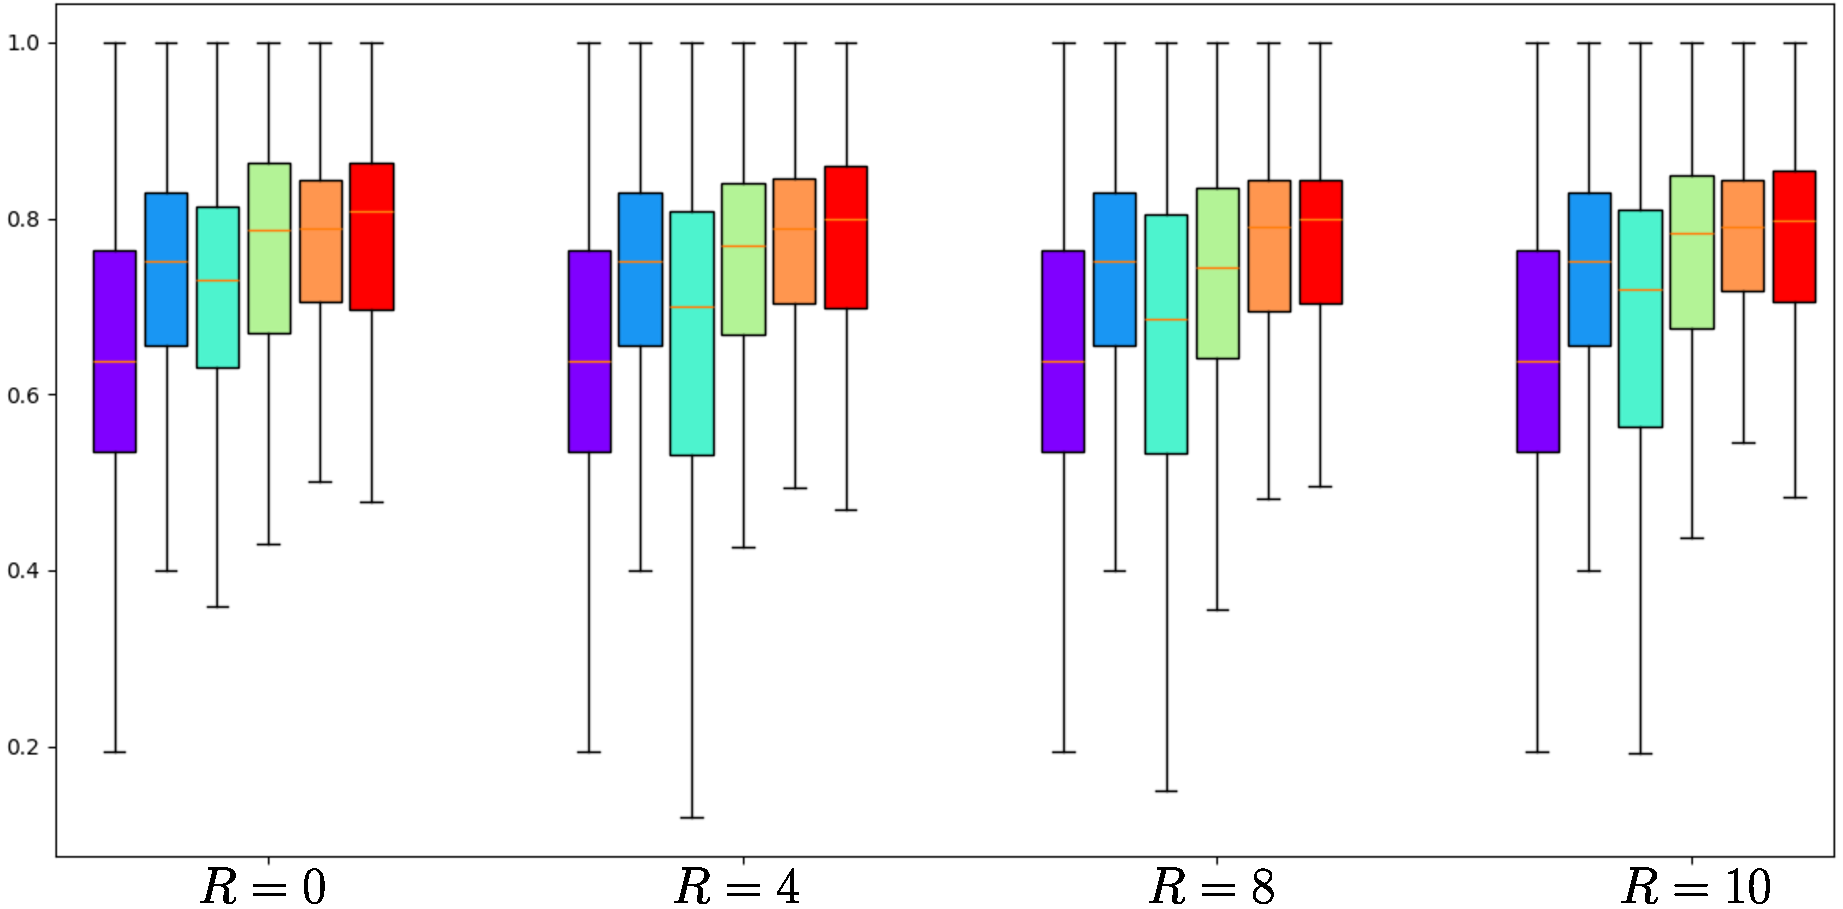
\includegraphics[width=\textwidth]{Boxplot_DiceScores_LV-Cavity.pdf}
    		\caption{Boxplot of the Dice scores for the LV cavity.} %on the fully sampled \emph{ACDC} test data
    		\label{fig:Boxplot_DiceScores_LV-Cavity}
	\end{subfigure}
	\\
	\begin{subfigure}{0.85\textwidth}
    		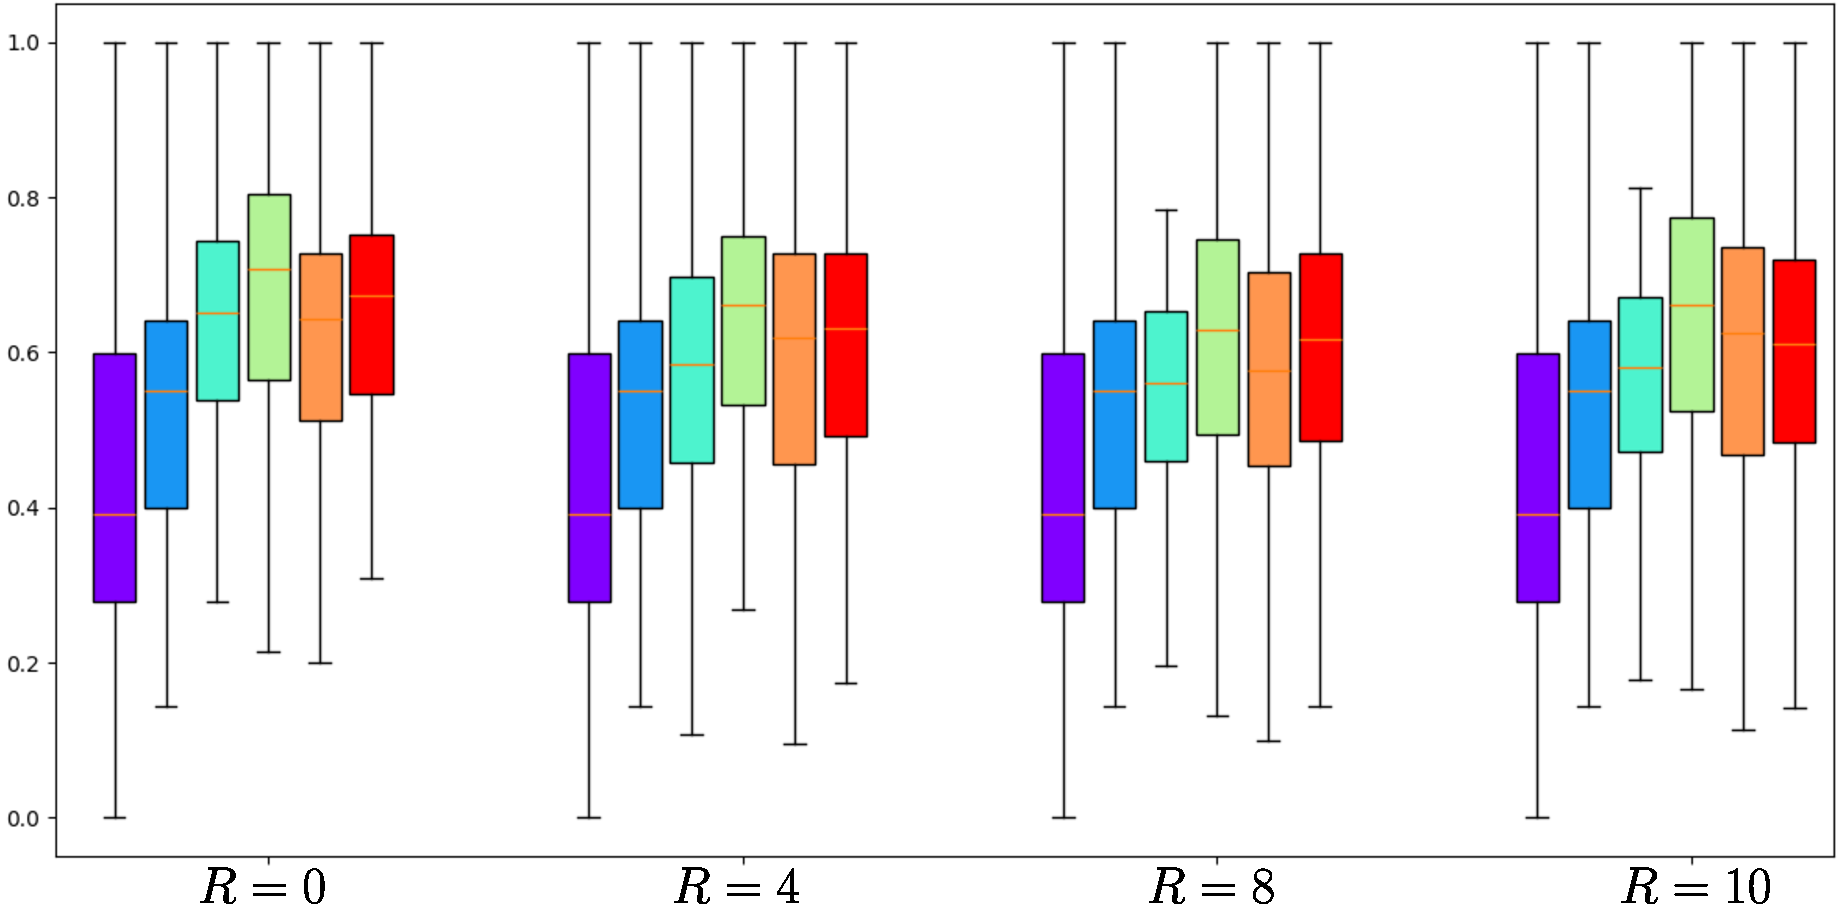
\includegraphics[width=\textwidth]{Boxplot_DiceScores_Myocardium.pdf}
    		\caption{Boxplot of the Dice scores for the myocardium.} %on the Acc4 \emph{ACDC} test data
    		\label{fig:Boxplot_DiceScores_Myocardium}
	\end{subfigure}
	\\
	\begin{subfigure}{0.85\textwidth}
    		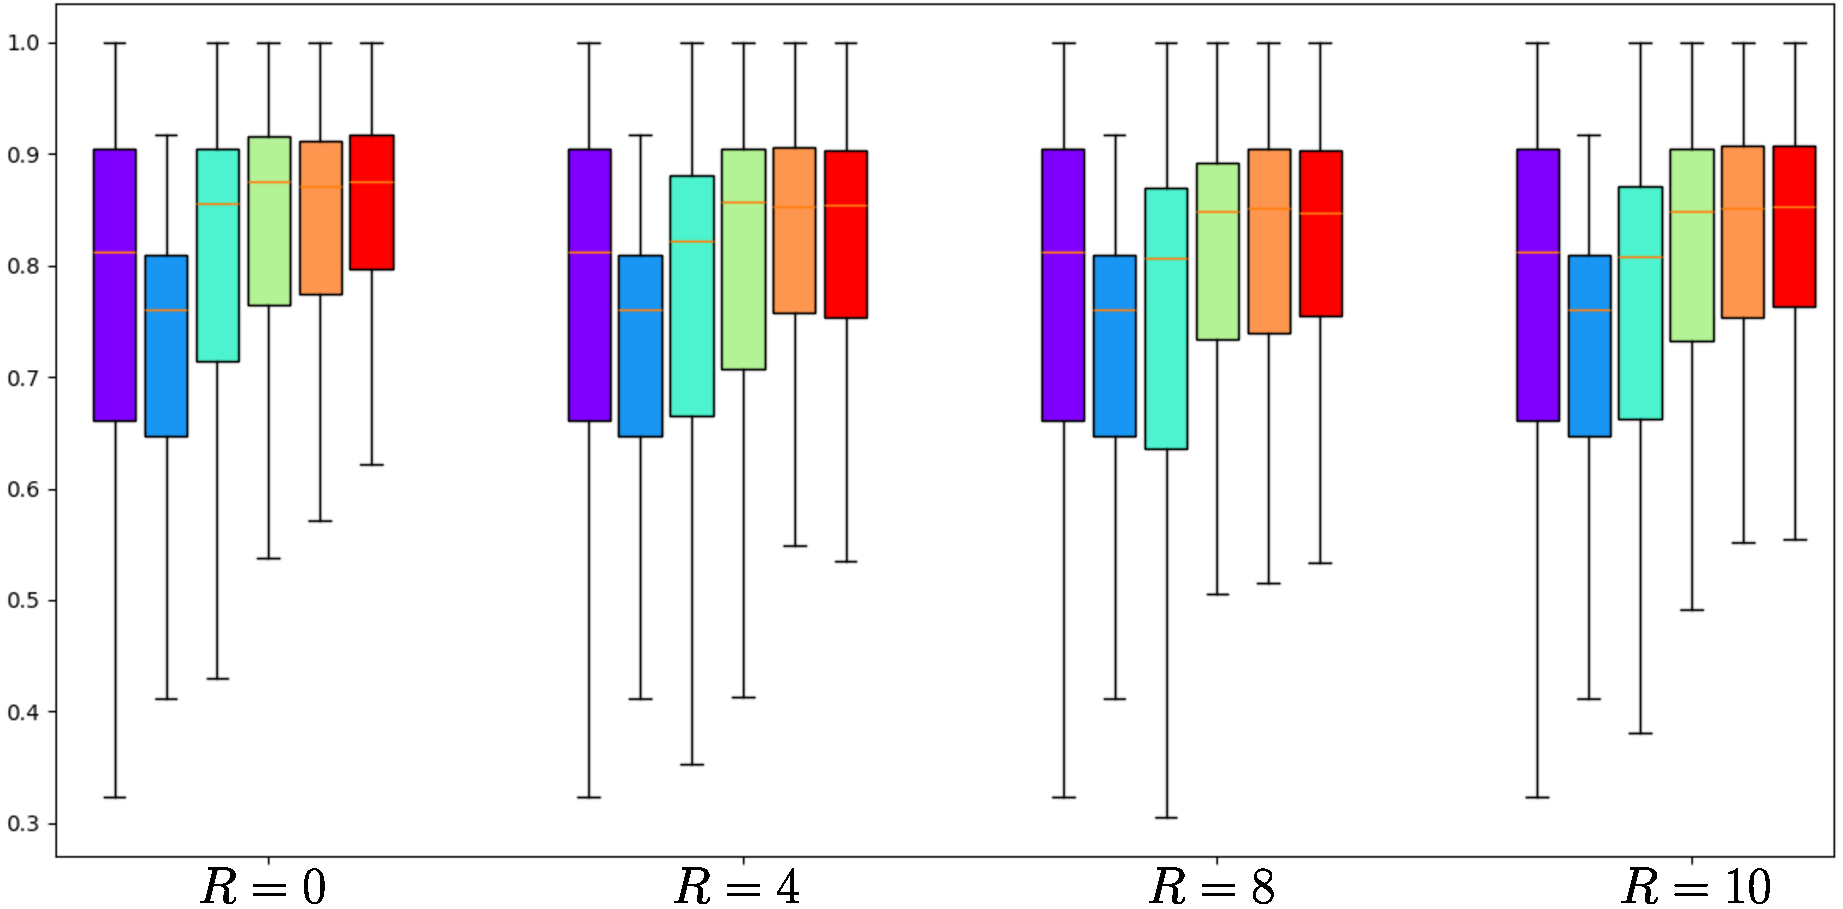
\includegraphics[width=\textwidth]{Boxplot_DiceScores_RV-Cavity.pdf}
    		\caption{Boxplot of the Dice scores for RV cavity.} %on the Acc8 \emph{ACDC} test data
    		\label{fig:Boxplot_DiceScores_RV-Cavity}
	\end{subfigure}
	\caption{Boxplots of Dice scores (split by label excluding the background) for all models on fully sampled ($R=0$) and subsampled ($R=4$, $R=8$, $R=10$) \emph{ACDC} test data. \legendsquare{violet}~Baseline, \legendsquare{teal}~\emph{NiftyReg}, \legendsquare{cyan}~\emph{VoxelMorph}, \legendsquare{lime}~\emph{Fourier-Net}, \legendsquare{orange}~\emph{Fourier-Net+}, \legendsquare{red}~\emph{4xFourier-Net+}}
	\label{fig:Boxplots_DiceScores}
\end{figure}


\subsubsection{Qualitative Results}
In order to explain the differences observed between the methods previously, a visual examination can be used. There, one can look at the warped images and segmentations as well as the generated displacement fields visualized in Figure~\ref{fig:TestExamples}. For all acceleration factors, an example moving and fixed image can be compared to the warped images by the different methods. For further analysis, the corresponding segmentations (with corresponding Dice scores) and displacement fields generated by the methods are given.\\
For $R=0$, \emph{Fourier-Net+} and \emph{4xFourier-Net+} have very localized displacements, centered on the cardiac region, leading to a very smooth warped segmentation compared to \emph{Fourier-Net} and \emph{VoxelMorph} where the cardiac labels mix in some regions. Despite this, \emph{Fourier-Net} still achieves the highest Dice score with an $16\%$ increase compared to the baseline. While \emph{NiftyReg} does produce a very smooth warped segmentation the actual displacements are very small and not localized on the cardiac region leading to the lowest Dice score of all methods.\\
For $R=4$, the image artifacts due to the subsampling are very apparent. The segmentations for the moving and fixed image obviously remain the same.
% despite the subsampling.
\emph{Fourier-Net+} and \emph{4xFourier-Net+} again have very smooth segmentations, however the displacements reflect the difficulties of adapting to subsampled data in becoming slightly less local. Surprisingly, \emph{NiftyReg} actually has a more localized displacement compared to the fully sampled data, however the segmentation looks less smooth and the Dice score is slightly lower. Somewhat similar, \emph{VoxelMorph} also has a more localized displacement leading to a smoother segmentation and a higher Dice score. The results of \emph{Fourier-Net} look overall very similar to the fully sampled case, perhaps with a bit more localized displacement leading to a smoother segmentation, although this does not lead to a better Dice Score.\\
For $R=8$, the displacements for all methods become more global due to the strong presence of image artifacts, however the Dice scores are higher than before for all methods. \emph{NiftyReg} even outperforms \emph{VoxelMorph} for the first time. This trend does not continue for $R=10$ however, were \emph{NiftyReg} is again far behind all other methods in terms of Dice with a very much more global displacement. \emph{VoxelMorph} seems to compensate more for the rippling artifacts present in the fixed image than for the change in the cardiac region as seen in the displacement. \emph{Fourier-Net}, \emph{Fourier-Net+} and \emph{4xFourier-Net+} do not share this behavior although their displacements also become more global and less focused on the cardiac region. The latter network has the highest Dice score for the first time managing an increase in Dice of about $16\%$ compared to the baseline for this specific case despite the heavy subsampling showing the robustness of the network.

\begin{figure}[H]
	\vspace{-1cm}
	\centering
	\graphicspath{{images/}{\main/images/}}
	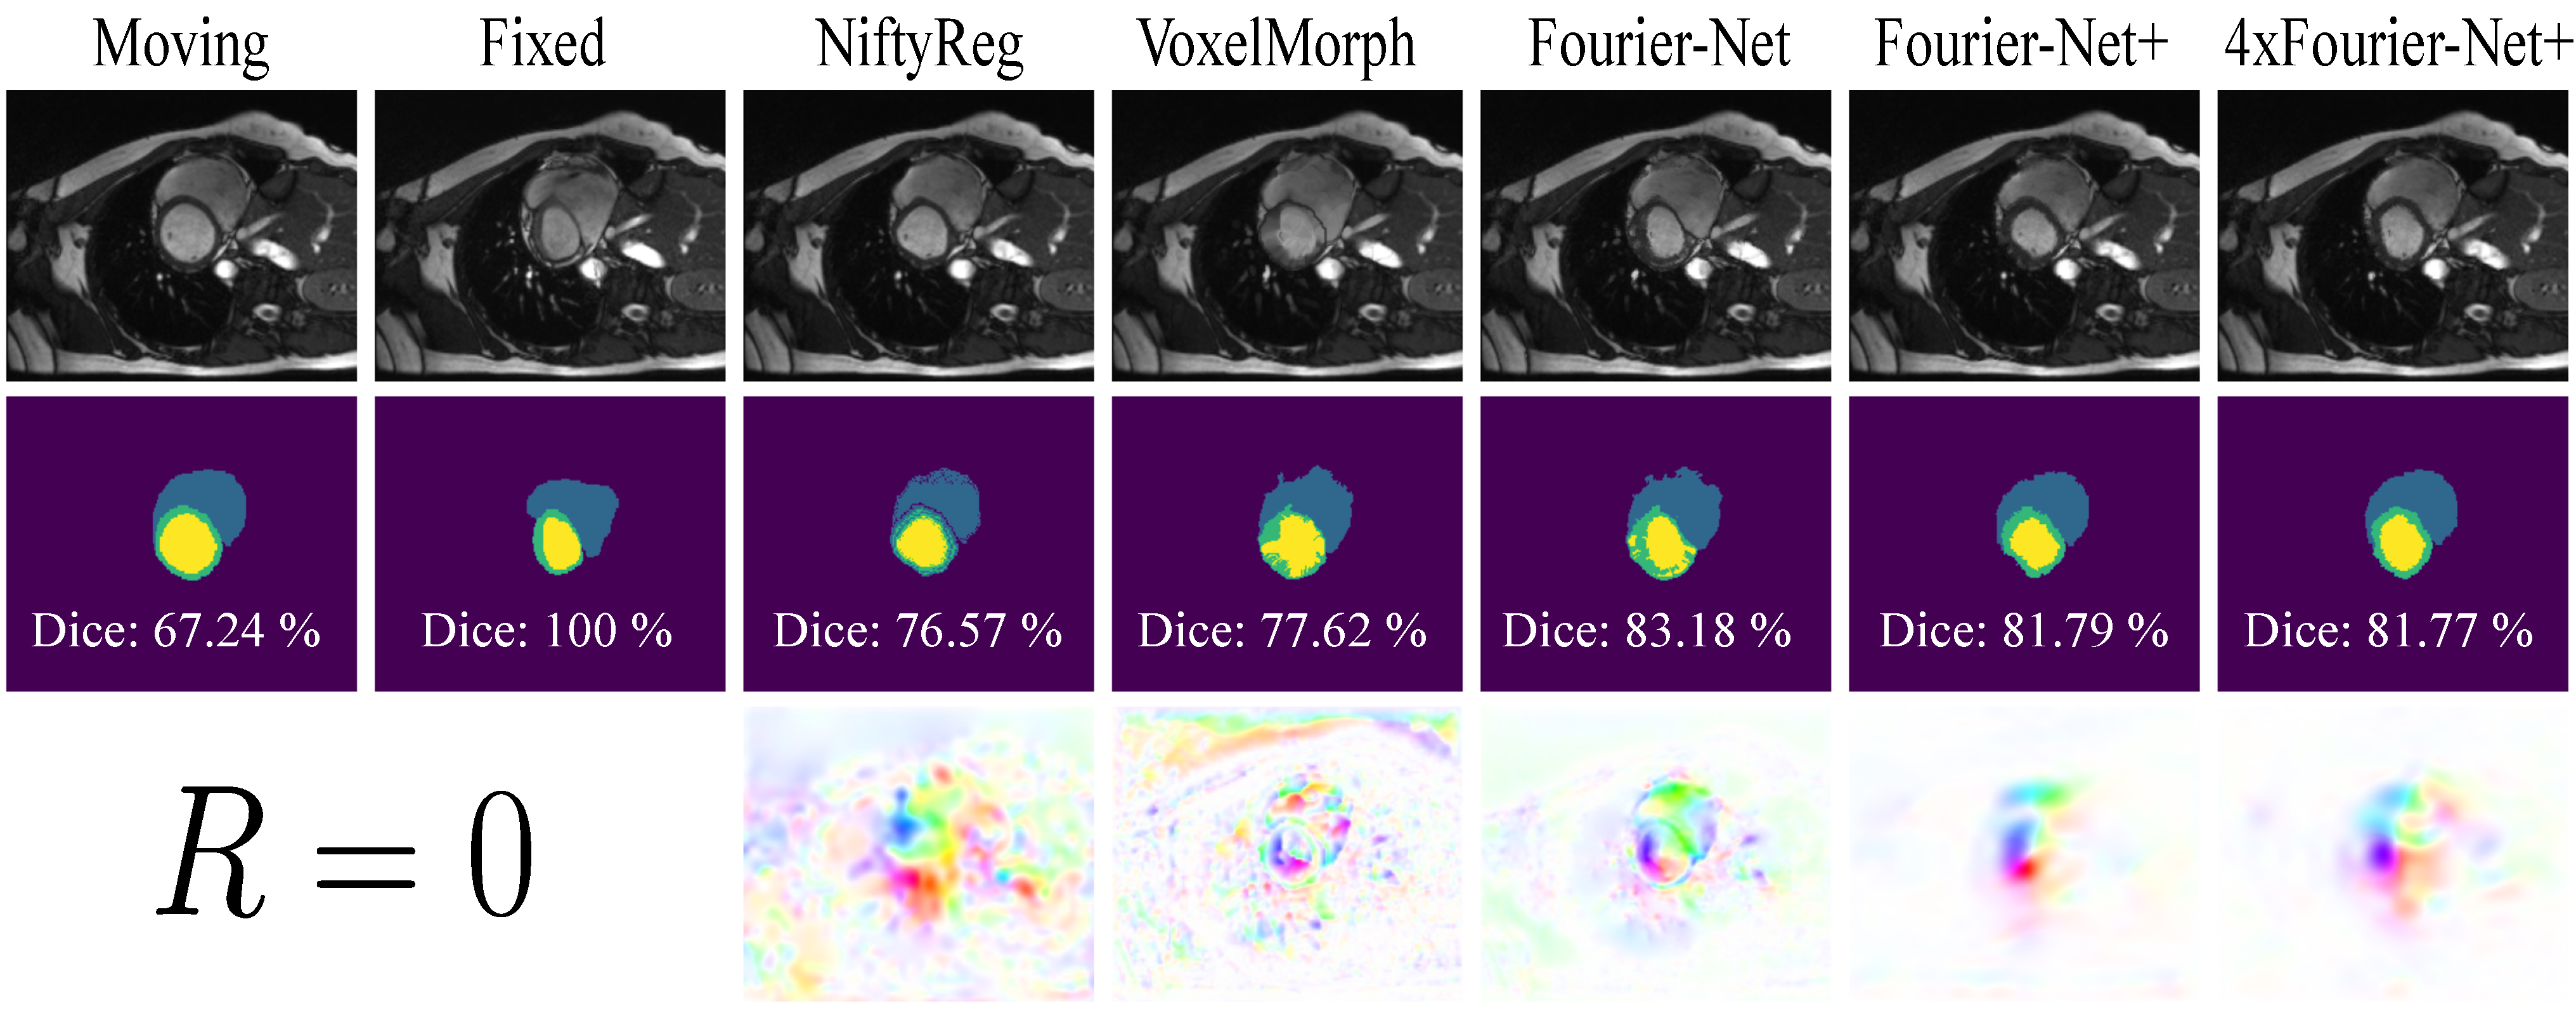
\includegraphics[width=.95\textwidth]{TestExamples_Mode0.pdf}
    	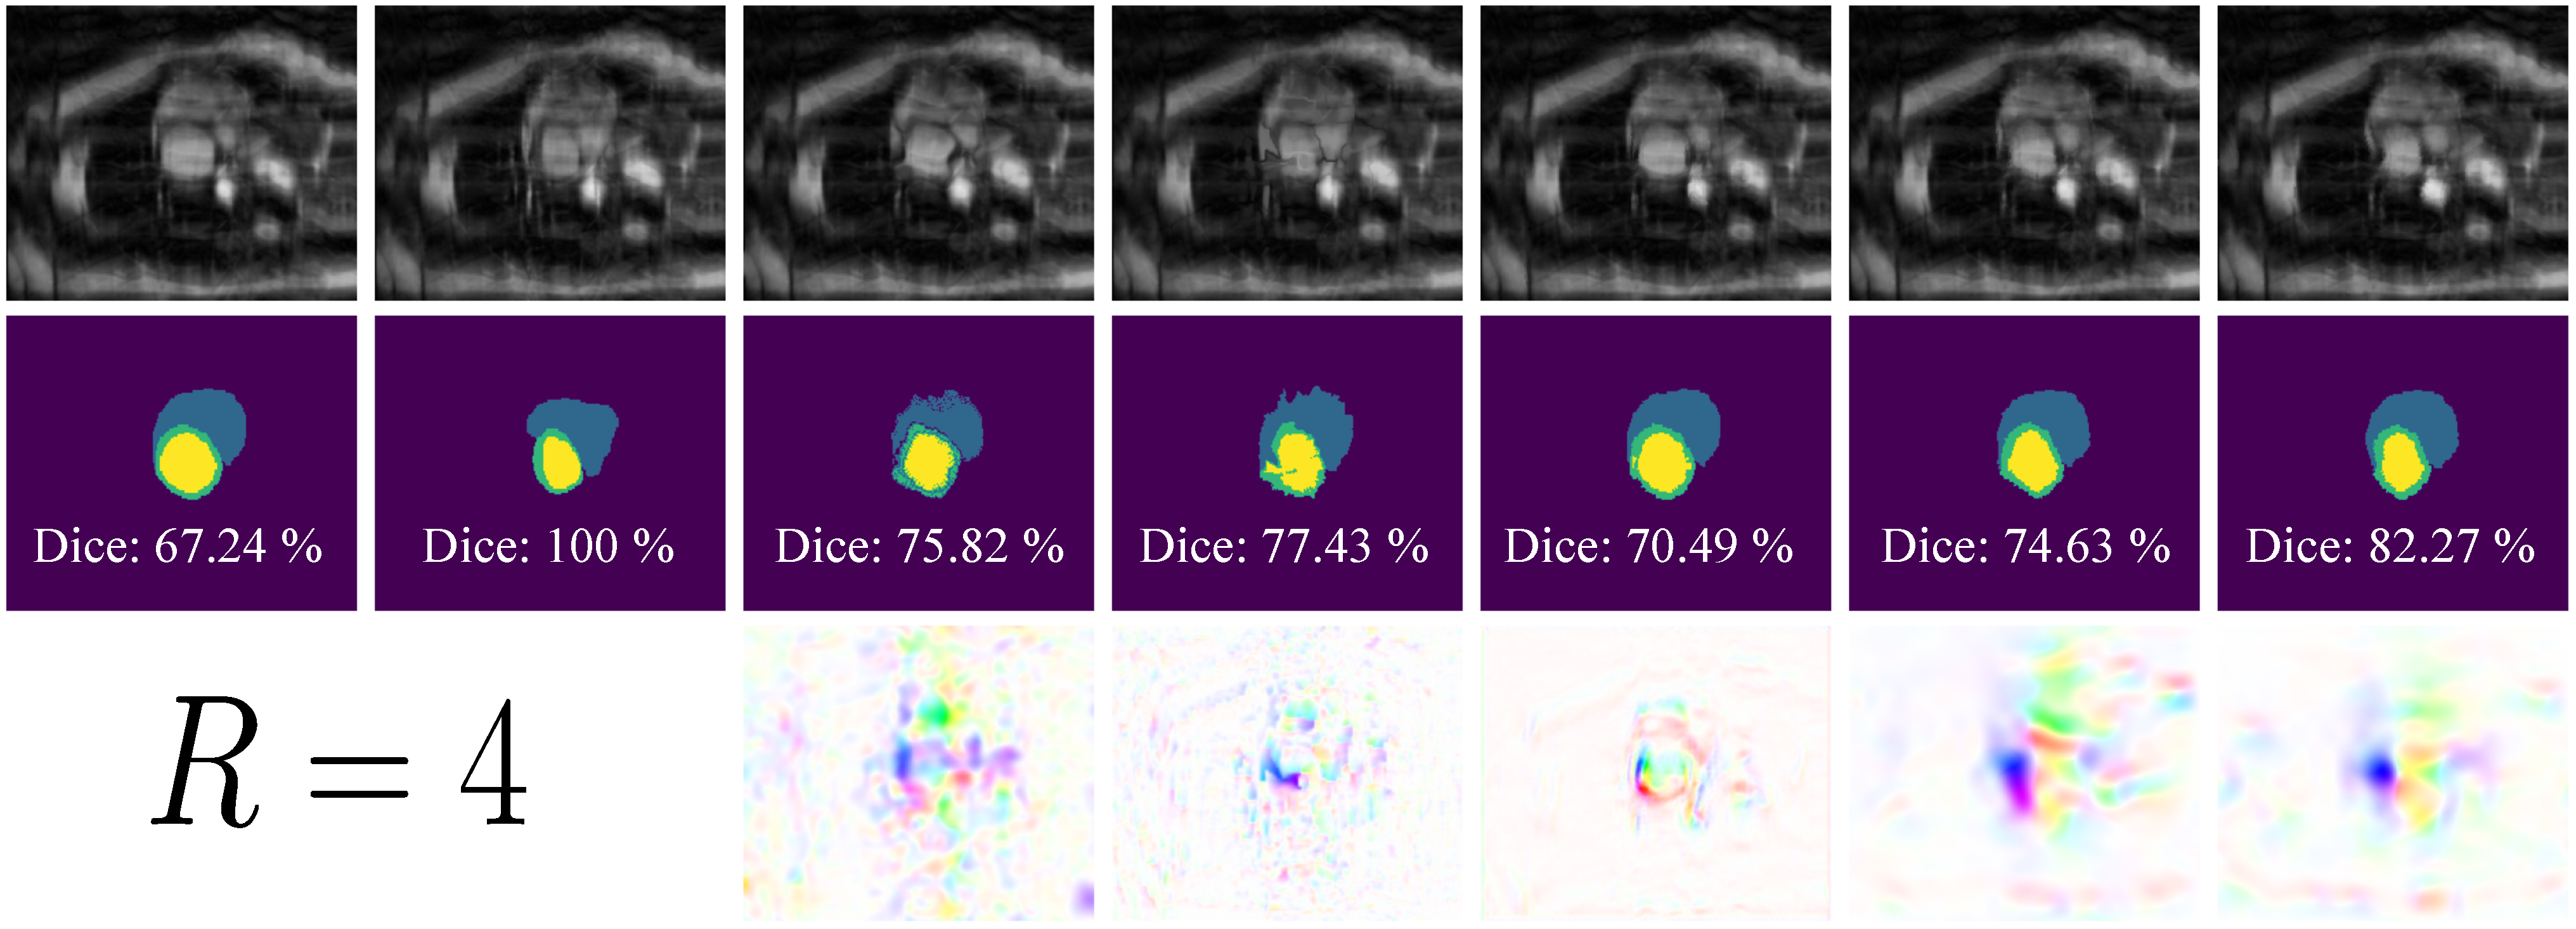
\includegraphics[width=.95\textwidth]{TestExamples_Mode1.pdf}
    	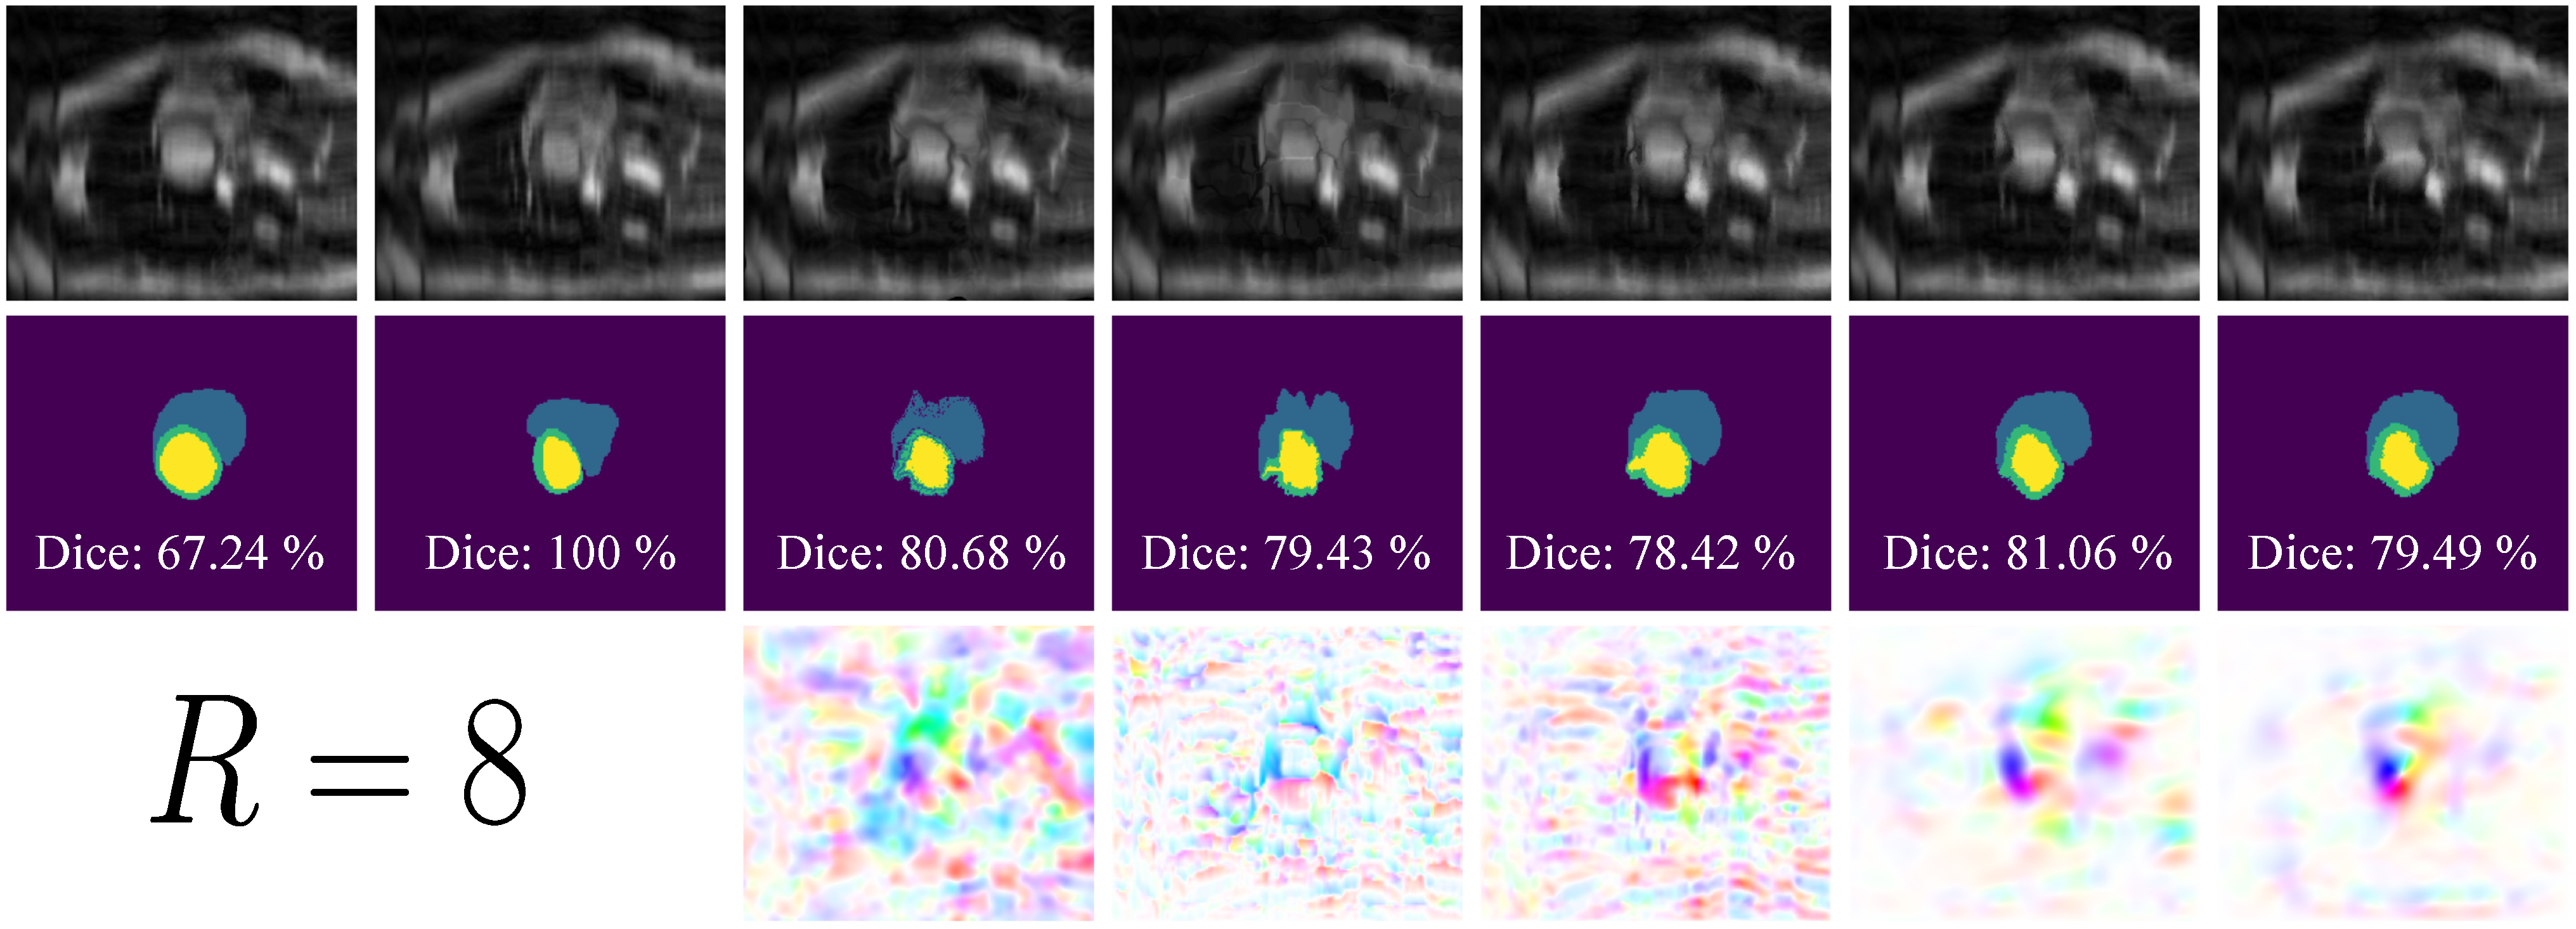
\includegraphics[width=.95\textwidth]{TestExamples_Mode2.pdf}
    	\includegraphics[width=.95\textwidth]{TestExamples_Mode3.pdf}	
	\caption{\small Examples of warped images, segmentations and flow fields for \emph{NiftiReg}, \emph{VoxelMorph}, \emph{Fourier-Net}, \emph{Fourier-Net+} and \emph{4xFourier-Net+} together with the original image pair from the fully sampled ($R=0$) and subsampled ($R=4$, $R=8$, $R=10$) \emph{ACDC} test data.}
	\label{fig:TestExamples}
\end{figure}


\section{Integration into a Motion-Compensated Reconstruction Pipeline} \label{Sec:ResultsIntegrationMotion-CompensatedReconstructionPipeline}
After assessing the registration performance of \emph{Fourier-Net}, \emph{Fourier-Net+} and \emph{4xFourier-Net+}, a final down-stream task to gauge the applicability of these networks was conducted in the form of an motion-compensated reconstruction pipeline where the networks are used to correct the moment between frames.

\subsubsection{K-Space Line Swapping} \label{SubSubSec:ResultsK-SpaceLineSwapping}
As discussed in section~\ref{SubSec:IntegrationMotion-CompensatedReconstructionPipeline}, the reconstruction pipeline was first tested with motion-corrupted data using k-space line swapping described in section~\ref{SubSec:SimulatedMotion}. The results are shown in Table~\ref{tab:ComparisonReconstructionCMRxReconLineSwapping} with blue marking the best results per metric (not present if all methods have the same performance) and red marking worse results than the baseline. \\
For $z=16$, performance decreases with higher acceleration. For $R=4$, \emph{Fourier-Net} has the highest HaarPSI and SSIM values, while \emph{VoxelMorph} has the highest PSNR. \emph{Fourier-Net+} on the other hand, has the lowest values for these metrics. All methods as well as the baseline have the same mean MSE value. Only for the third decimal point in the standard deviation a small difference between the different methods is visible (note that the MSE values are already multiplied by a factor of 100). %\\
For $R=8$, \emph{Fourier-Net} again has the highest value for the HaarPSI, followed by \emph{Fourier-Net+}, as well as the highest SSIM value, followed by \emph{4xFourier-Net+} which also has the highest PSNR. While the MSE values are again very close, \emph{4xFourier-Net+} has a slightly lower mean value than the other methods.%\\
For $R=10$, \emph{4xFourier-Net+} performs best for all metrics with \emph{Fourier-Net+} having the same mean MSE value. \emph{VoxelMorph} and \emph{Fourier-Net} perform worse than baseline for the HaarPSI with the latter also having lower PSNR and SSIM values than the baseline.\\
For $z=32$ and $R=4$, \emph{Fourier-Net} performs best for all metrics, while \emph{4xFourier-Net+} performs worse than baseline for PSNR, SSIM and MSE. For $R=8$, \emph{Fourier-Net+} has the highest HaarPSI, PSNR and SSIM values followed by \emph{Fourier-Net}. The mean MSE value is again the same for all methods and slightly lower than the baseline. For $R=10$, \emph{Fourier-Net+} again performs best for all metrics. Only \emph{Fourier-Net} has a lower SSIM than the baseline.

\begin{table}[H] %tpb
	%\footnotesize
	\small
	\centering
	\caption{Reconstruction results \emph{VoxelMorph}, \emph{Fourier-Net}, \emph{Fourier-Net+} and \emph{4xFourier-Net+} on the \emph{CMRxRecon} test data for $R=4$, $R=8$ and $R=10$ as well as an baseline without motino-correction. The best results for each metric and subsampling are highlighted in blue, while values worse than the unaligned baseline are marked with red.}
	\label{tab:ComparisonReconstructionCMRxReconLineSwapping}
	\begin{tabularx}{\textwidth}{c Y Y Y Y Y} 
		\toprule
		 & \multirow{2}{*}{Methods} & \multicolumn{4}{c}{Motion-correction for $z=16$ swapped k-space lines} \\
		\cmidrule(lr){3-6} 
		 & & $\%$ HaarPSI $\uparrow$ & PSNR [dB] $\uparrow$ & $\%$ SSIM $\uparrow$ & MSE (m) $\downarrow$\\
		
		% 4x Accelerated (R=4) 				 		
		\midrule
		\multirow{5}{*}{\rotatebox{90}{$R=4$}} & Baseline & $56.884 \pm 8.129$ & $28.703 \pm 2.388$ & $78.079 \pm 5.887$ & $0.160 \pm 0.125$ \\  
		 & VoxelMorph & $56.909 \pm 8.118$ & \textcolor{blue}{$28.709 \pm 2.404$} & $78.090 \pm 5.903$ & $0.160 \pm 0.126$ \\  
		 & Fourier-Net & \textcolor{blue}{$56.918 \pm 8.160$} & $28.706 \pm 2.401$ & \textcolor{blue}{$78.123 \pm 5.893$} & $0.160 \pm 0.126$ \\  
		 & Fourier-Net+ & \textcolor{red}{$56.854 \pm 8.158$} & \textcolor{red}{$28.699 \pm 2.399$} & \textcolor{red}{$78.071 \pm 5.951$} & $0.160 \pm 0.126$ \\   
		 & \mbox{4xFourier-Net+} & $56.903 \pm 8.109$ & $28.702 \pm 2.380$ & $78.085 \pm 5.877$ & $0.160 \pm 0.125$ \\  
		
		% 8x Accelerated (R=8) 
		\midrule
		\multirow{5}{*}{\rotatebox{90}{$R=8$}} & Baseline & $53.318 \pm 7.641$ & $28.104 \pm 2.383$ & $77.311 \pm 5.934$ & $0.183 \pm 0.139$ \\  
		 & VoxelMorph & $53.342 \pm 7.687$ & $28.110 \pm 2.405$ & $77.341 \pm 5.900$ & $0.183 \pm 0.139$ \\  
		 & Fourier-Net & \textcolor{blue}{$53.394 \pm 7.681$} & $28.128 \pm 2.398$ & \textcolor{blue}{$77.416 \pm 5.927$} & $0.183 \pm 0.138$ \\  
		 & Fourier-Net+ & $53.388 \pm 7.664$ & $28.118 \pm 2.404$ & $77.398 \pm 5.906$ & $0.183 \pm 0.138$ \\   
		 & \mbox{4xFourier-Net+} & $53.376 \pm 7.688$ & \textcolor{blue}{$28.133 \pm 2.398$} & $77.402 \pm 5.936$ & \textcolor{blue}{$0.182 \pm 0.138$} \\ 
		 	 
		% 10x Accelerated (R=10) 		 		
		\midrule		
		\multirow{5}{*}{\rotatebox{90}{$R=10$}} & Baseline & $52.212 \pm 7.388$ & $27.906 \pm 2.364$ & $77.175 \pm 5.886$ & $0.191 \pm 0.141$ \\  
		 & VoxelMorph & \textcolor{red}{$52.211 \pm 7.393$} & $27.907 \pm 2.368$ & $77.194 \pm 5.863$ & $0.191 \pm 0.140$ \\  
		 & Fourier-Net & \textcolor{red}{$52.192 \pm 7.361$} & \textcolor{red}{$27.895 \pm 2.362$} & \textcolor{red}{$77.160 \pm 5.815$} & $0.191 \pm 0.139$ \\  
		 & Fourier-Net+ & $52.240 \pm 7.379$ & $27.924 \pm 2.357$ & $77.244 \pm 5.866$ & \textcolor{blue}{$0.189 \pm 0.139$} \\   
		 & \mbox{4xFourier-Net+} & \textcolor{blue}{$52.272 \pm 7.330$} & \textcolor{blue}{$27.931 \pm 2.349$} & \textcolor{blue}{$77.262 \pm 5.816$} & \textcolor{blue}{$0.189 \pm 0.137$} \\ 
		 
		 \midrule	
		 & & \multicolumn{4}{c}{Motion-correction for $z=32$ swapped k-space lines} \\
		% 4x Accelerated (R=4) 				 		
		\midrule
		\multirow{5}{*}{\rotatebox{90}{$R=4$}} & Baseline & $52.711 \pm 7.673$ & $27.506 \pm 2.180$ & $74.379 \pm 5.869$ & $0.203 \pm 0.130$ \\  
		 & VoxelMorph & $52.747 \pm 7.658$ & $27.512 \pm 2.188$ & $74.349 \pm 5.900$ & $0.203 \pm 0.129$ \\  
		 & Fourier-Net & \textcolor{blue}{$52.802 \pm 7.708$} & \textcolor{blue}{$27.536 \pm 2.197$} & \textcolor{blue}{$74.421 \pm 5.937$} & \textcolor{blue}{$0.202 \pm 0.128$} \\  
		 & Fourier-Net+ & $52.725 \pm 7.724$ & $27.522 \pm 2.198$ & $74.366 \pm 5.892$ & $0.203 \pm 0.129$ \\   
		 & \mbox{4xFourier-Net+} & $52.711 \pm 7.718$ & \textcolor{red}{$27.500 \pm 2.205$} & \textcolor{red}{$74.353 \pm 5.986$} & \textcolor{red}{$0.204 \pm 0.132$} \\  
		
		% 8x Accelerated (R=8) 
		\midrule
		\multirow{5}{*}{\rotatebox{90}{$R=8$}} & Baseline & $50.071 \pm 7.259$ & $27.153 \pm 2.199$ & $74.033 \pm 5.844$ & $0.221 \pm 0.138$ \\  
		 & VoxelMorph & $50.091 \pm 7.301$ & $27.164 \pm 2.198$ & $74.060 \pm 5.890$ & $0.220 \pm 0.138$ \\  
		 & Fourier-Net & $50.152 \pm 7.325$ & $27.178 \pm 2.202$ & $74.094 \pm 5.826$ & $0.220 \pm 0.140$ \\  
		 & Fourier-Net+ & \textcolor{blue}{$50.159 \pm 7.362$} & \textcolor{blue}{$27.196 \pm 2.221$} & \textcolor{blue}{$74.119 \pm 5.853$} & $0.220 \pm 0.141$ \\   
		 & \mbox{4xFourier-Net+} & $50.128 \pm 7.276$ & $27.165 \pm 2.201$ & $74.054 \pm 5.842$ & $0.220 \pm 0.137$ \\ 
		 	 
		% 10x Accelerated (R=10) 		 		
		\midrule		
		\multirow{5}{*}{\rotatebox{90}{$R=10$}} & Baseline & $49.193 \pm 7.022$ & $27.013 \pm 2.170$ & $73.971 \pm 5.788$ & $0.227 \pm 0.143$ \\  
		 & VoxelMorph & $49.241 \pm 7.047$ & $27.026 \pm 2.179$ & $73.976 \pm 5.795$ & $0.227 \pm 0.142$ \\  
		 & Fourier-Net & $49.255 \pm 7.011$ & $27.024 \pm 2.168$ & \textcolor{red}{$73.952 \pm 5.793$} & $0.227 \pm 0.141$ \\  
		 & Fourier-Net+ & \textcolor{blue}{$49.296 \pm 7.001$} & \textcolor{blue}{$27.045 \pm 2.172$} & \textcolor{blue}{$74.028 \pm 5.784$} & \textcolor{blue}{$0.226 \pm 0.140$} \\   
		 & \mbox{4xFourier-Net+} & $49.287 \pm 7.066$ & $27.032 \pm 2.176$ & $74.022 \pm 5.820$ & $0.227 \pm 0.143$ \\ 
		 \bottomrule
	\end{tabularx}
\end{table}


\subsubsection{Simulated Lung Movement} \label{SubSubSec:ResultsLungMovement}
As discussed in section~\ref{SubSec:IntegrationMotion-CompensatedReconstructionPipeline} a second test with simulated non-linear lung motion was conducted. Results are shown in Table~\ref{tab:ComparisonReconstructionCMRxReconLungMovement} with blue marking the best results per metric. For $R=4$, \emph{Fourier-Net} has the highest HaarPSI, PSNR and SSIM value followed by \emph{Fourier-Net+} and \emph{4xFourier-Net+}. \emph{Fourier-Net} also has the lowest MSE value again followed by \emph{Fourier-Net+} and \emph{4xFourier-Net+}. \emph{VoxelMorph} performs better than the baseline, but lacks behind \emph{Fourier-Net}, \emph{Fourier-Net+} and \emph{4xFourier-Net+}. For $R=8$, \emph{Fourier-Net+} overtakes \emph{Fourier-Net} for HaarPSI, PSNR, SSIM and MSE followed by \emph{4xFourier-Net+}. \emph{VoxelMorph} is again the weakest method. Overall, the metrics are very much affected by the increased subsampling as the HaarPSI is about $4 \%$ lower for the methods compared to $R=4$. The PSNR, SSIM and MSE are not effected quite as much, but are also lower in the case of PSNR, SSIM by about $1 \%$ and the MSE is higher by about $0.03 \cdot 10^{-3}$. The results for $R=10$ are very similar to $R=8$. \emph{Fourier-Net+} again has the highest HaarPSI, PSNR and SSIM followed by \emph{4xFourier-Net+} and \emph{Fourier-Net}. This time the decrease in metrics from $R=10$ compared to $R=8$ is not quite as large (about $0.5 \%$, $0.2 \%$ and $0.1 \%$ respectively). \emph{Fourier-Net+} also has the lowest MSE again followed by \emph{4xFourier-Net+} similar to $R=8$ as the metrics barely changed.

\begin{table}[h] %tpb
	%\footnotesize
	\small
	\centering
	\caption{Reconstruction results \emph{VoxelMorph}, \emph{Fourier-Net}, \emph{Fourier-Net+} and \emph{4xFourier-Net+} on the \emph{CMRxRecon} test data for $R=4$, $R=8$ and $R=10$ as well as an baseline without motion-compensation. The best results for each metric and subsampling are highlighted in blue, while values worse than the unaligned baseline are marked with red.}
	\label{tab:ComparisonReconstructionCMRxReconLungMovement}
	\begin{tabularx}{\textwidth}{c Y Y Y Y Y} 
		\toprule
		 & \multirow{2}{*}{Methods} & \multicolumn{4}{c}{Metrics} \\
		\cmidrule(lr){3-6} 
		  & & $\%$ HaarPSI $\uparrow$ & PSNR [dB] $\uparrow$ & $\%$ SSIM $\uparrow$ & MSE (m) $\downarrow$\\
		
		% 4x Accelerated (R=4) 				 		
		\midrule
		\multirow{5}{*}{\rotatebox{90}{$R=4$}} & Baseline & $28.882 \pm 3.802$ & $23.291 \pm 1.654$ & $70.375 \pm 4.467$ & $0.504 \pm 0.197$ \\  
		 & VoxelMorph & $54.177 \pm 7.495$ & $28.347 \pm 2.369$ & $79.873 \pm 4.878$ & $0.174 \pm 0.138$ \\ 
		 & Fourier-Net & \textcolor{blue}{$59.886 \pm 8.876$} & \textcolor{blue}{$29.399 \pm 2.766$} & \textcolor{blue}{$82.731 \pm 5.296$} & \textcolor{blue}{$0.141 \pm 0.127$} \\  
		 & Fourier-Net+ & $59.868 \pm 8.824$ & $29.303 \pm 2.761$ & $82.572 \pm 5.037$ & $0.146 \pm 0.142$  \\    
		 & \mbox{4xFourier-Net+} & $59.884 \pm 8.875$ & $29.365 \pm 2.764$ & $82.704 \pm 5.293$ & $0.144 \pm 0.141$ \\ 
		
		% 8x Accelerated (R=8) 
		\midrule
		\multirow{5}{*}{\rotatebox{90}{$R=8$}} & Baseline & $28.572 \pm 3.773$ & $23.173 \pm 1.686$ & $70.603 \pm 4.533$ & $0.519 \pm 0.207$ \\  
		 & VoxelMorph & $50.537 \pm 7.213$ & $27.596 \pm 2.460$ & $78.848 \pm 5.121$ & $0.209 \pm 0.161$ \\ 
		 & Fourier-Net & $55.326 \pm 8.415$ & $28.465 \pm 2.846$ & $81.383 \pm 5.489$ & $0.191 \pm 0.129$ \\  
		 & Fourier-Net+ & \textcolor{blue}{$55.406 \pm 8.432$} & \textcolor{blue}{$28.519 \pm 2.799$} & \textcolor{blue}{$81.447 \pm 5.478$} & \textcolor{blue}{$0.178 \pm 0.162$} \\    
		 & \mbox{4xFourier-Net+} & $55.402 \pm 8.463$ & $28.508 \pm 2.916$ & $81.436 \pm 5.329$ & $0.181 \pm 0.153$ \\ 
		 	 
		% 10x Accelerated (R=10) 		 		
		\midrule		
		\multirow{5}{*}{\rotatebox{90}{$R=10$}} & Baseline & $28.486 \pm 3.766$ & $23.132 \pm 1.695$ & $70.742 \pm 4.436$ & $0.524 \pm 0.211$ \\  
		 & VoxelMorph & $49.072 \pm 6.854$ & $27.331 \pm 2.417$ & $78.756 \pm 4.962$ & $0.220 \pm 0.163$ \\ 
		 & Fourier-Net & $54.012 \pm 8.046$ & $28.217 \pm 2.758$ & $81.224 \pm 5.323$ & $0.193 \pm 0.162$ \\  
		 & Fourier-Net+ & \textcolor{blue}{$54.025 \pm 8.053$} & \textcolor{blue}{$28.228 \pm 2.745$} & \textcolor{blue}{$81.264 \pm 5.331$} & \textcolor{blue}{$0.189 \pm 0.164$} \\    
		 & \mbox{4xFourier-Net+} & $54.016 \pm 8.064$ & $28.223 \pm 2.691$ & $81.236 \pm 5.237$ & $0.191 \pm 0.148$ \\ 
		 \bottomrule
	\end{tabularx}
\end{table}

\subsubsection{Qualitative Results}
Similar to the registration performance on the \emph{ACDC} dataset in section~\ref{SubSec:ResultsComparisonSubsampling}, visual examples can give insights and reasons for trends observed in the metrics. These examples can be seen for \emph{VoxelMorph}, \emph{Fourier-Net}, \emph{Fourier-Net+} and \emph{4xFourier-Net+} in Figure~\ref{fig:ResultsReconstruction}. There, the reconstruction results using the different networks for motion-compensation and the motion-corrupted baseline are compared to the fully sampled ground truth image using error maps for all three subsampling factors $R=4$, $R=8$ and $R=10$.\\
In the top row, the images for the ground truth, the subsampled and motion-corrupted baseline, as well as the reconstructions using \emph{VoxelMorph}, \emph{Fourier-Net}, \emph{Fourier-Net+} and \emph{4xFourier-Net+} are shown. In the top right corner of the images, the SSIM calculated in comparison to the ground truth is shown. It should be noted that all images were croped around the cardiac region for better visualization of the details in the images. Lastly, in the bottom row, the error maps show the differences between the images and the ground truth. The color bar on the left indicates the severity of the deviation going from blue (no/small difference) to yellow (large difference).\\
For $R=4$, as seen before in Table~\ref{tab:ComparisonReconstructionCMRxReconLungMovement}, \emph{Fourier-Net} has the highest SSIM. But what about the visual look? Starting with the motion-corrupted baseline, it is clear that the image is affected by artifacts. The cardiac region looks blurred and distorted with a big tear being visible. This is most like the result of the motion-corruption as the subsampling only leads to blurring and aliasing artifacts, which are also visible. Continuing with \emph{VoxelMorph}, it is clear that the reconstruction has not been able to restore the image as parts of the cardiac region are still blurred and a small tear is also visible. This can also be seen in the error map where subsampling artifacts can still be seen. Despite the superior performance in terms of metrics, there are still some subsampling artifacts visible for \emph{Fourier-Net}. The cardiac region, however, looks far better compared to \emph{VoxelMorph}, though still slightly blurred when compared to the ground truth. Next up is \emph{Fourier-Net+}, where more artifacts are again present. The cardiac region is again strongly blurred which can also be seen in the error map. \emph{4xFourier-Net+} also shows some blurring but not as much as \emph{Fourier-Net+}. Despite this the SSIM for the image is slightly lower.\\
For $R=8$, \emph{Fourier-Net+} has the highest SSIM followed by \emph{4xFourier-Net+}. \emph{VoxelMorph} again shows a lot of artifacts with a small tear ans strong blurring in the cardiac region similar to the baseline. \emph{Fourier-Net} on the other hand has far less artifacts though the whole image still appears quite blurred. The image for \emph{Fourier-Net+} looks less blurred however artifacts from the subsampling are still visible. \emph{4xFourier-Net+} again looks more like \emph{Fourier-Net} before with stronger blurring and failing to remove some of the motion artifacts. However, it still has a slightly better SSIM.\\
For $R=10$, \emph{Fourier-Net+} again has the highest SSIM, although the value is lower than for $R=8$. \emph{VoxelMorph} shows artifacts similar to before, though without a tear in the cardiac region this time. \emph{Fourier-Net} also has a lot of artifacts distorting the image similar to \emph{VoxelMorph}. \emph{Fourier-Net+} is mostly free of artifacts except for some blurring. \emph{4xFourier-Net+} similar to \emph{Fourier-Net} has large blurring artifacts in the cardiac region and the contrast seems to be slightly different.

\begin{figure}[H] %tpb
	\centering
	\includegraphics[width=\linewidth]{./Images/ResultsReconstruction_mode1.pdf} 
	\includegraphics[width=\linewidth]{./Images/ResultsReconstruction_mode2.pdf}
	\includegraphics[width=\linewidth]{./Images/ResultsReconstruction_mode3.pdf}
	\caption{Visual results of the reconstruction pipeline for \emph{VoxelMorph}, \emph{Fourier-Net}, \emph{Fourier-Net+} and \emph{4xFourier-Net+} as well as the ground truth image and the motion-corrupted baseline on the \emph{CMRxRecon} test data for $R=4$, $R=8$ and $R=10$.}
	\label{fig:ResultsReconstruction}
\end{figure}
%%%%%%%%%%%%%%%%%%%%%%%
%%%%%  Discussion %%%%%
%%%%%%%%%%%%%%%%%%%%%%%

\chapter{Discussion} \label{Ch:Discussion}
After presenting the results of the experiments described in section~\ref{Sec:Experiments}, it is time to discuss the implications of the results. First, the parameter tests conducted on the \emph{ACDC} dataset and then the evaluation of the reconstruction pipeline on the \emph{CMRxRecon} dataset.

\section{Parameter Tests on the ACDC Dataset} \label{Sec:DiscussionParameterTestsACDC}
For the first tests, the performance of \emph{Fourier-Net}, \emph{Fourier-Net+} and \emph{4xFourier-Net+} was evaluated on the \emph{ACDC} dataset alongside different parameter tests and ablation studies. These results now need to be analyzed and interpreted.

\subsection{Fourier-Net versus Fourier-Net+} \label{SubSec:DiscussionFourier-NetvsFourier-Net+ACDC}
In a first comparative study, the performance of \emph{Fourier-Net}, \emph{Fourier-Net+} and \emph{4xFourier-Net+} was compared in section ~\ref{SubSec:ResultsFourier-NetvsFourier-Net+ACDC} together with their respective memory consumption.\\
For the dense displacement variants, the diffeomorphic transform increases the performance slightly for \emph{Fourier-Net} and \emph{4xFourier-Net}, but decreases for \emph{Fourier-Net+}. The times between the baseline and diffeomorphic versions are comparable.
The results for the band-limited versions are very similar with \emph{Fourier-Net} and \emph{Fourier-Net+} performing slightly worse  with the diffeomorphism, while \emph{4xFourier-Net} performs better.  These changes are not consistent with the dense displacement versions, however, the band-limited \emph{4xFourier-Net} version might be an outlier, as all of the other models are not affected as much by the diffeomorphic transform. The percentage of non-positive Jabobian determinants decreases for all diffeomorphic variants, which is as expected.\\
Overall, the dense displacement versions perform better in terms of Dice (with and without the background label), SSIM and MSE for all models. This is to be expected as the dense displacement versions can use all of the available k-space data for the registration task, while the band-limited versions have only a limited amount of k-space data, directly impacting and limiting their performance. The dense displacement are only slightly better in the SSIM and MSE metrics, however the difference is not quite as large as with the Dice scores. As the differences between the frames is not quite as large, the weaker registration performance does not impact this metric as much as the Dice score, which is focused on the moving cardiac region.\\
Only in terms of the percentage of non-positive Jabobian determinants does the band-limited displacement actually perform better as the band-limiting probably allows for only a smaller deformation. However, the difference is still very small, especially for the diffeomorhpic versions, and it could be argued that a better registration performance at the cost of some image folding is an acceptable trade-off. \\
In terms of inference time the dense displacement variants are surprisingly slightly faster despite having a larger encoder, however all of the model are in the low milliseconds ($<40$~ms). Lastly, the memory consumption needs to be addressed. The dense displacment variants have a larger encoder as discussed before and thus have a lot more parameters, especially for the more optimized \emph{Fourier-Net+} and \emph{4xFourier-Net} (about 5 times more). The number of Mult-Adds and the amount of total memory are more than doubled (almost tripled for \emph{4xFourier-Net}) for the dense displacement versions compared to those with a band-limited displacement across all models. This shows that a larger network produces better results, however for certain applications where efficiency is needed a smaller, but slightly worse, network might be more beneficial.\\
To summarize, \emph{Fourier-Net} performs best for the band-limited displacement, while \emph{4xFourier-Net+} works better with a dense displacement. While the dense displacements overall provide the better performance, the memory cost is enormous. Utilizing a diffeomorphic transform does not generally lead to a better performance.

\subsection{Starting Channel Size} \label{SubSec:DiscussionStartingChannelsACDC}
One of the most important parameters for the networks is the channel size. A larger channel size means more features, but also a larger network. The results from section~\ref{SubSec:ResultsStartingChannelsACDC} show that memory efficiency and registration performance for \emph{Fourier-Net+} and \emph{4xFourier-Net+} cannot be optimized at the same time - there is a clear trade-off between the two. For both \emph{Fourier-Net+} and \emph{4xFourier-Net+} a clear increase in performance with larger channel sizes can be observed as more features are utilized. The percentage of non-positive Jabobian determinants also decreases as the registration performance increases, likely due to better/more features enabling a smoother and better displacement field to be generated by the models. The inference time is not impacted by channel size. The memory however increases exponentially when doubling the channel sizes as all layers are effected, not just the starting one as the name might suggest. Thus, the number of parameters drastically increases with starting size leading to an increase in Mult-Add and thus overall memory. \\
To summarize, as the channel sizes increase, making the network larger, the performance also increases. While this effect is quite large at the beginning, it plateaus rather quickly. This trade-off and the diminishing returns imply that there is a sweet spot where the network is still efficient while maintaining a good performance. The starting channel size 16 was thus chosen for the following experiments.

\subsection{Fourier-Transform Crop Size} \label{SubSec:DiscussionFTCropSize}
The FT crop is specific to \emph{Fourier-Net+} and \emph{4xFourier-Net+}, however, the size of the crop has a mayor impact on the input images as a smaller crop leads to more compressed images, but also better memory usage. Similarly to channel size before, the results in section~\ref{SubSec:ResultsFTCropSize} indicate that there is no sweet-spot to be found that maximizes both memory efficiency and registration performance. The latter decreases drastically with a smaller crop size. This is to be expected as the smaller FT drop compresses the images more  making an accurate registration harder. Interestingly, the percentage of non-positive Jabobian determinants actually decreases for smaller crop sizes, perhaps because the displacements on the compressed images are not as extreme and thus more smooth. Inference time also seems to decrease slightly with a smaller crop, although the time measurements are not quite consistent.\\
The number of parameters does not change for different crop sizes as the networks themselves do not change, however the number of Mult-Adds and the total memory still change with the image size. Both decrease with a larger crop size as the image gets smaller. This effect is again not linear as a reduction in image size yields a larger reduction in memory for large crop sizes before flattening out for smaller ones. 

\subsection{Comparison with VoxelMorph} \label{SubSec:DiscussionComparisonVoxelMorph}
As a comparison with a very common unsupervised registration network, the registration performance and memory imprint of \emph{Fourier-Net}, \emph{Fourier-Net+} and \emph{4xFourier-Net+} was compared in section~\ref{SubSec:ResultsComparisonVoxelMorph} to \emph{VoxelMorph}. Overall, \emph{4xFourier-Net+} is the only model that is truly more efficient and has a better performance in terms of Dice than \emph{VoxelMorph}, as \emph{Fourier-Net+} is more efficient, but not necessarily better in terms of Dice score, while \emph{Fourier-Net} is far superior in registration performance (as measured by the Dice score), but less efficient in terms of memory consumption.

\subsection{Dense Displacements} \label{SubSec:DiscussionDenseDisplacements}
As a final ablation study, the difference between a band-limited and a dense displacement in \emph{Fourier-Net}, \emph{Fourier-Net+} and \emph{4xFourier-Net+} was tested in section \ref{SubSec:ResultsDenseDisplacementAcc}. The results for the band-limited networks are consistently worse (or in the best case just as good) compared to their dense versions across all acceleration factors for Dice, SSIM and MSE. The band-limiting of the displacement helps with avoiding folding and in most cases decrease inference time, however at the expense of registration performance. Our hypothesis that the advantage of the dense displacement compared to the band-limited displacement disappears for accelerated data does not seem to hold as the dense networks outperform the band-limited ones, though the difference is small in some cases. In the end, the larger dense networks perform better, but also require more memory. Thus, similar to the previous experiments, a balance between performance and memory efficiency has to be found.

\subsection{Comparison on Subsampled Data} \label{SubSec:DiscussionComparisonSubsampling}
In section~\ref{SubSec:ResultsComparisonSubsampling} the registration performance of \emph{Fourier-Net}, \emph{Fourier-Net+} and \emph{4xFourier-Net+} was compared to an unaligned baseline as well as \emph{NiftyReg} and \emph{VoxelMorph} for four different reduction factors. To summarize the results, \emph{Fourier-Net+} is the fastest method for all acceleration levels while \emph{NiftyReg} is far behind all other methods in execution time as it is not machine learning based. \emph{VoxelMorph} performs best in terms of SSIM and MSE for all acceleration factors, however it also has the highest percentage of non-positive Jabobian determinants by a large margin indicating potential folding artifacts. \emph{4xFourier-Net+} performs best in terms of Dice with the background label except for $R=0$ while consistently having the lowest percentage of non-positive Jabobian determinants with a mean value under $0.004\%$ for all acceleration factors. \emph{Fourier-Net+} performs well in terms of Dice (with and without the background label), however it does not manage to surpass the other \emph{Fourier-Net} variants despite having the second lowest percentage of non-positive Jabobian determinants across the acceleration factors. \emph{Fourier-Net} performs best in terms of Dice without the background label for all acceleration level as well as in Dice with the background for $R=0$. \emph{NiftyReg} consistently performs worse than the baseline in terms of Dice (with and without the background) across all acceleration factors while having decent SSIM and MSE values. The performance, in general, decreased for all methods for higher acceleration factors as seen in the Dice metric, however, perhaps counter-intuitively, the SSIM is highest and the MSE the lowest for the $R=10$ baseline with only $R=4$ breaking the trend. This shows once again that image similarity metrics are not completely objective when it comes to evaluating registration performance across different acceleration factors.


\section{Integration into a Motion-Compensated Reconstruction Pipeline} \label{Sec:DiscussionIntegrationMotion-CompensatedReconstructionPipeline}
As a final down-stream task, the usage of \emph{Fourier-Net}, \emph{Fourier-Net+} and \emph{4xFourier-Net+} as part of an motion-compensated reconstruction pipeline was evaluated.

%% remove subsections once most of the text is done
\subsection{Domain Translation} \label{SubSec:DiscussionDomainTranslation}
First, the domain translation between the \emph{ACDC} and \emph{CMRxRecon} datasets was tested for the networks. As seen in section~\ref{SubSec:ResultsDomainTranslation}, the results for all networks are very similar. The mean values of all metrics for \emph{Fourier-Net+} and \emph{4xFourier-Net+} were the same with only a small difference in inference time between the networks. The same is true for the MSE and percentage of non-positive Jabobian determinants of \emph{Fourier-Net}, however, the SSIM is slightly better for the version trained on \emph{ACDC} with a difference of about $0.2 \%$. Thus, overall, no domain gap was observed.

\subsection{Reconstruction Pipeline} \label{SubSec:DiscussionReconstructionPipeline}
Next, a reconstruction pipeline was build and tested using two different methods for simulating motion in an MRI image.

\subsubsection{K-Space Line Swapping}
As expected, the performance for $z=16$ is better than $z=32$ as the latter contains more artifacts. In both cases, performance also decreases for higher acceleration as expected. Overall, the results for $z=32$ are far easier to interpret. \emph{Fourier-Net} performs best for $R=4$ with \emph{4xFourier-Net+} underperforming, while \emph{Fourier-Net+} performs best for $R=8$ and $R=10$. For $z=16$, the results are far less cohesive. \emph{Fourier-Net} performs best in HaarPSI and SSIM for $R=4$ and $R=8$, but underperforms for $R=10$ while \emph{4xFourier-Net+} is best in PSNR and MSR for $R=8$ and performs best across all metrics for $R=10$. \emph{Fourier-Net+} underperforms for $R=4$, but is decent for the other reduction factors. The MSE metrics overall is barely usable as the differences between the images are not captured by the metric (differences in mean values often in the sixth decimal point). However, even the other metrics are very similar for each reduction factor which implies that the reconstruction does not have a large impact on image quality. This is perhaps due to motion artifacts mostly blurring the images and still being too tame. These potential problem were addressed in the next test.

\subsubsection{Simulated Lung Movement}
Simulated Lung Movement...

\section{Limitations and Outlook}
While the registration performance of \emph{Fourier-Net}, \emph{Fourier-Net+} and \emph{4xFourier-Net+} was very good on the \emph{ACDC} dataset, beating traditional algorithms and other neural networks, further comparisons with other more advanced networks such as LAPNet~\cite{LAPNet} on another cardiac dataset would be interesting. While three different reduction factors were used for most of the experiment, even higher acceleration could be an interesting test for the networks adaptability. In general, all network versions were specific to their acceleration. A test for the generalization of the learned properties would be interesting as the networks could be applied to another acceleration as they were trained on. In the best case a network could be trained on all of the data with different reduction factors to hopefully generalize the results for all accelerations. This would make an application to real world problems far easier as a single network could be used for a range of different data.Changes and additions to the network architecture and training of \emph{Fourier-Net}, \emph{Fourier-Net+} and \emph{4xFourier-Net+} might also be interesting to further optimize the performance.\\
A problem with evaluating the reconstruction pipeline are the different networks training performance. As a new network is trained for each reduction factor, the performance might not just be impacted by the acceleration of the image, but also by the networks training. As the latter is non-deterministic in nature it can be hard in some cases to separate whether the network simply underperformed compared to its usual potential or whether the task is truly much more challenging. As an example, \emph{Fourier-Net+} in some cases outperformed its cascaded version \emph{4xFourier-Net+} which is unexpected. In most cases the smaller, more efficient \emph{Fourier-Net+} would show a decrease in performance compared to the larger \emph{Fourier-Net} and \emph{4xFourier-Net+}, however, in some cases due to fluctuation in the training, this assumption would not hold. This further complicates accurately interpreting the results obtained in the different experiments.\\
\emph{Fourier-Net}, \emph{Fourier-Net+} and \emph{4xFourier-Net+} are very versatile networks that can be used for different tasks and data regarding image registration. In the future... 
%%%%%%%%%%%%%%%%%%%%%%%
%%%%%  Conclusion %%%%%
%%%%%%%%%%%%%%%%%%%%%%%

\chapter{Conclusion} \label{Ch:Conclusion}
In this thesis, the usage of \emph{Fourier-Net}, \emph{Fourier-Net+} and \emph{4xFourier-Net+} for efficient and fast registration of subsampled MRI data was explored. This research question was approached from multiple different angles examining registration both directly, comparing the networks to traditional algorithms and other neural networks, as well as indirectly as part of a motion-compensated reconstruction pipeline. \\
After training the network on subsampled MRI data, multiple experiments were described to examine the research question. These included multiple ablation studies and parameter tests on the \emph{ACDC} dataset followed by downstream tests on the \emph{CMRxRecon} dataset. While the latter was for testing the applicability of the networks, the parameter tests were used to find optimal model parameters for \emph{Fourier-Net}, \emph{Fourier-Net+} and \emph{4xFourier-Net+}. Then their registration performance was compared to \emph{NiftyReg}, a traditional registration algorithm, and \emph{VoxelMorph}, a state-of-the-art neural network.\\
For the second part of experiments, the three networks were used as part of an motion-compensated reconstruction pipeline. For this, the \emph{CMRxRecon} dataset was used as it contained the needed k-space data and subsampling masks. We simulated motion for a downstream test using a motion-compensated reconstruction pipeline. Two different approaches were used to simulate mis-triggering and non-linear lung motion between frames. These were then reconstructed using a pipeline with neural networks for motion-compensation. The three networks were again compared to \emph{VoxelMorph} in this downstream test.

%% ------------------------------------------------------------------------

% Format des Chapterheades:
\renewcommand\chapterlinesformat[3]{\vspace{-.9cm}#3\vspace{.6cm}}

%% ------------------------------------------------------------------------
%% Literatur- und Abkuerzungsverzeichnis
%% ------------------------------------------------------------------------
\printbibliography

%%% ----------------------------------
%%   Abkuerzungsverzeichnis.tex
%% ----------------------------------
\chapter*{Abkürzungsverzeichnis}
\label{sec:Abkuerzungsverzeichnis}
\footnotesize
\begin{acronym}[]

\end{acronym}

%% ------------------------------------------------------------------------
%% Anhang
%% ------------------------------------------------------------------------

% Format des Chapterheades:
\renewcommand\chapterlinesformat[3]{\vspace{-.9cm}\appendixname\ #2\\*\vspace{.6cm}#3\vspace{.6cm}}

% \appendix
% %% ----------------------------------
%%   Anhang.tex
%% ----------------------------------

\chapter{Titel Anhang A}


\end{document}
